\documentclass[12pt,letterpaper]{report}

% ==================== PAQUETES ====================
\usepackage[spanish,es-tabla]{babel}
\usepackage[utf8]{inputenc}
\usepackage[T1]{fontenc}
\usepackage{amsmath,amssymb,amsthm}
\usepackage{graphicx}
\usepackage[left=2.5cm,right=2.5cm,top=3cm,bottom=3cm]{geometry}
\usepackage{setspace}
\usepackage{fancyhdr}
\usepackage{titlesec}
\usepackage{tocloft}
\usepackage[hidelinks]{hyperref}
\usepackage{float}
\usepackage{caption}
\usepackage{subcaption}
\usepackage{enumitem}
\usepackage{csquotes}

% ==================== CONFIGURACIONES ====================
\onehalfspacing

\pagestyle{fancy}
\fancyhf{}
\fancyhead[L]{\leftmark}
\fancyhead[R]{\thepage}
\renewcommand{\headrulewidth}{0.5pt}

\titleformat{\chapter}[display]
  {\normalfont\huge\bfseries}{\chaptertitlename\ \thechapter}{20pt}{\Huge}
\titlespacing*{\chapter}{0pt}{0pt}{40pt}

\renewcommand{\contentsname}{Índice}
\renewcommand{\listfigurename}{Índice de Figuras}
\renewcommand{\listtablename}{Índice de Tablas}
\renewcommand{\bibname}{Referencias}

\numberwithin{equation}{chapter}
\numberwithin{figure}{chapter}
\numberwithin{table}{chapter}

% ==================== INFORMACIÓN DEL DOCUMENTO ====================
\title{Integradora de Matemáticas para la Ingeniería II}
\author{Reyes Vargas Isael Alejandro}
\date{\today}

% ==================== INICIO DEL DOCUMENTO ====================
\begin{document}

% ==================== PORTADA ====================
\begin{titlepage}
    \centering

    \begin{minipage}{0.4\textwidth}
        \centering
        
\includegraphics[width=0.7\textwidth]{img/logo-utez.png}
    \end{minipage}
    \hfill
    \begin{minipage}{0.4\textwidth}
        \centering
        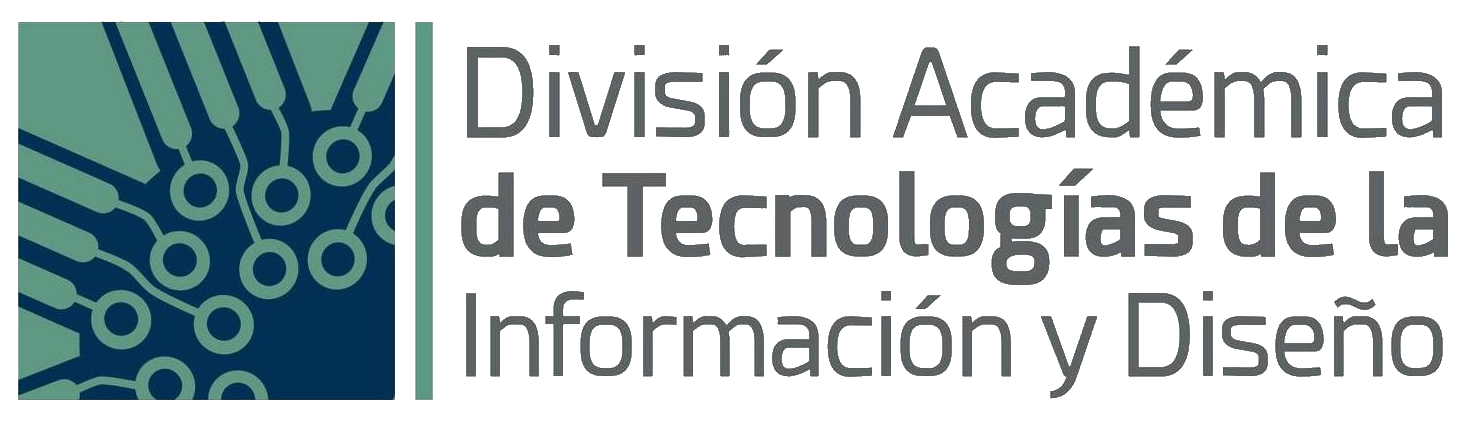
\includegraphics[width=0.7\textwidth]{img/logo-datid.png}
    \end{minipage}

    \vspace{1cm}

    {\Large\textbf{UNIVERSIDAD TECNOLÓGICA EMILIANO ZAPATA}}\\[0.5cm]
    {\large División Académica de Tecnologías de la Información y Diseño}\\[0.5cm]
    {\large Ingeniería en Desarrollo y Gestión de Software}\\[2cm]

    \rule{\linewidth}{0.5mm}\\[0.4cm]
    {\huge\bfseries Integradora de Matemáticas\\[0.2cm]para la Ingeniería II}\\[0.2cm]
    \rule{\linewidth}{0.5mm}\\[2cm]

    {\Large\textbf{Proyecto Integrador}}\\[1.5cm]

    \begin{minipage}{0.8\textwidth}
        \begin{flushleft}
            \textbf{Materia:}\\
            Matemáticas para Ingeniería II\\[0.5cm]

            \textbf{Profesor:}\\
            Dr. Jorge Yusef Colin Castillo\\[0.5cm]

            \textbf{Grupo:} 8 C\\[0.5cm]

            \textbf{Integrantes del Equipo:}\\
            \begin{itemize}[leftmargin=1cm]
                \item Reyes Vargas Isael Alejandro
            \end{itemize}
        \end{flushleft}
    \end{minipage}

    \vfill

    {\large Emiliano Zapata, Morelos, México}\\
    {\large \today}
\end{titlepage}

% ==================== ÍNDICES ====================
\tableofcontents
\cleardoublepage

\listoffigures
\cleardoublepage

% ==================== UNIDAD I ====================
\chapter{Unidad I: Ecuaciones Diferenciales de Primer Orden}

Las ecuaciones diferenciales constituyen una de las ramas más fecundas de las matemáticas aplicadas. A diferencia del álgebra elemental, donde se busca determinar valores numéricos desconocidos, una ecuación diferencial postula una relación entre una función incógnita y sus derivadas. Su resolución permite modelar con rigor procesos cuyos estados evolucionan de manera continua: el crecimiento de una población, la descarga de un condensador, la propagación de un virus en una red digital o la dinámica de un sistema de control. El estudio sistemático de estas ecuaciones es, por consiguiente, un requisito indispensable para cualquier ingeniero que aspire a construir modelos predictivos del comportamiento de sistemas reales.

\section{Introducción a las Ecuaciones Diferenciales}

\subsection{Contexto Histórico}

El origen formal de las ecuaciones diferenciales se remonta al siglo XVII, cuando Isaac Newton y Gottfried Wilhelm Leibniz desarrollaron de manera independiente el cálculo infinitesimal. Newton formuló sus \textit{fluxiones} para describir el movimiento de cuerpos celestes, estableciendo relaciones entre posiciones y velocidades que hoy reconocemos como ecuaciones diferenciales ordinarias. Leibniz, por su parte, introdujo la notación $\dfrac{dy}{dx}$ que persiste hasta la actualidad, dotando al campo de una herramienta simbólica de enorme claridad operativa.

Durante el siglo XVIII, Leonhard Euler sistematizó métodos de solución numérica y analítica, mientras que Daniel Bernoulli resolvió la ecuación de la cuerda vibrante, dando lugar al análisis de ecuaciones en derivadas parciales. Jacob Bernoulli estudió una clase particular de ecuaciones no lineales que hoy llevan su nombre. En el siglo XIX, Augustin-Louis Cauchy estableció la teoría de existencia y unicidad de soluciones, y Henri Poincaré fundó el análisis cualitativo, abriendo la puerta al estudio de sistemas dinámicos y caos determinista.

En el contexto de la ingeniería de software, el interés contemporáneo por las ecuaciones diferenciales ha crecido con la expansión de sistemas de simulación, aprendizaje automático basado en ecuaciones de estado y modelado de flujos de información en redes de computadoras.

\subsection{Definición Formal, Orden y Linealidad}

Una \textbf{ecuación diferencial ordinaria} (EDO) es una ecuación que involucra una función incógnita de una sola variable independiente y al menos una de sus derivadas. La forma general es:
\begin{equation*}
F\!\left(x,\, y,\, y',\, y'',\, \ldots,\, y^{(n)}\right) = 0
\end{equation*}

donde $x$ es la variable independiente, $y = y(x)$ es la función incógnita e $y^{(k)}$ denota su $k$-ésima derivada.

\textbf{Orden} de una EDO es el orden de la derivada de mayor grado que aparece en la ecuación. Así, $y'' + 3y' - y = \sin(x)$ es de segundo orden.

\textbf{Linealidad:} Una EDO de orden $n$ es \textbf{lineal} si puede escribirse en la forma:
\begin{equation*}
a_n(x)\,y^{(n)} + a_{n-1}(x)\,y^{(n-1)} + \cdots + a_1(x)\,y' + a_0(x)\,y = g(x)
\end{equation*}

donde los coeficientes $a_k(x)$ y el término $g(x)$ son funciones de la variable independiente únicamente; la función incógnita $y$ y sus derivadas aparecen en forma lineal, sin productos entre ellas ni como argumento de funciones no lineales. Si alguna de estas condiciones se viola, la ecuación es \textbf{no lineal}.

\subsection{Ejercicios: Comprobación de Soluciones (Bloque 1)}

A continuación se presentan ejercicios de verificación: dada una ecuación diferencial, se integra para obtener la solución general y se comprueba que ésta la satisface mediante sustitución directa.

\textbf{Ejercicio 1.} $y' - x^2 - 2x = 0$

\textit{Solución:}

\begin{align*}
\dfrac{dy}{dx} &= x^2 + 2x \\[4pt]
dy &= (x^2 + 2x)\,dx
\end{align*}

Integrando ambos miembros:
\[
\int dy = \int (x^2 + 2x)\,dx \implies y = \dfrac{x^3}{3} + x^2 + c
\]

Verificación: derivando la solución obtenida,
\[
y' = x^2 + 2x
\]

Sustituyendo en la ecuación original:
\[
\boxed{x^2 + 2x - x^2 - 2x = 0 \implies 0 = 0 \quad \checkmark}
\]

\begin{figure}[H]
    \centering
    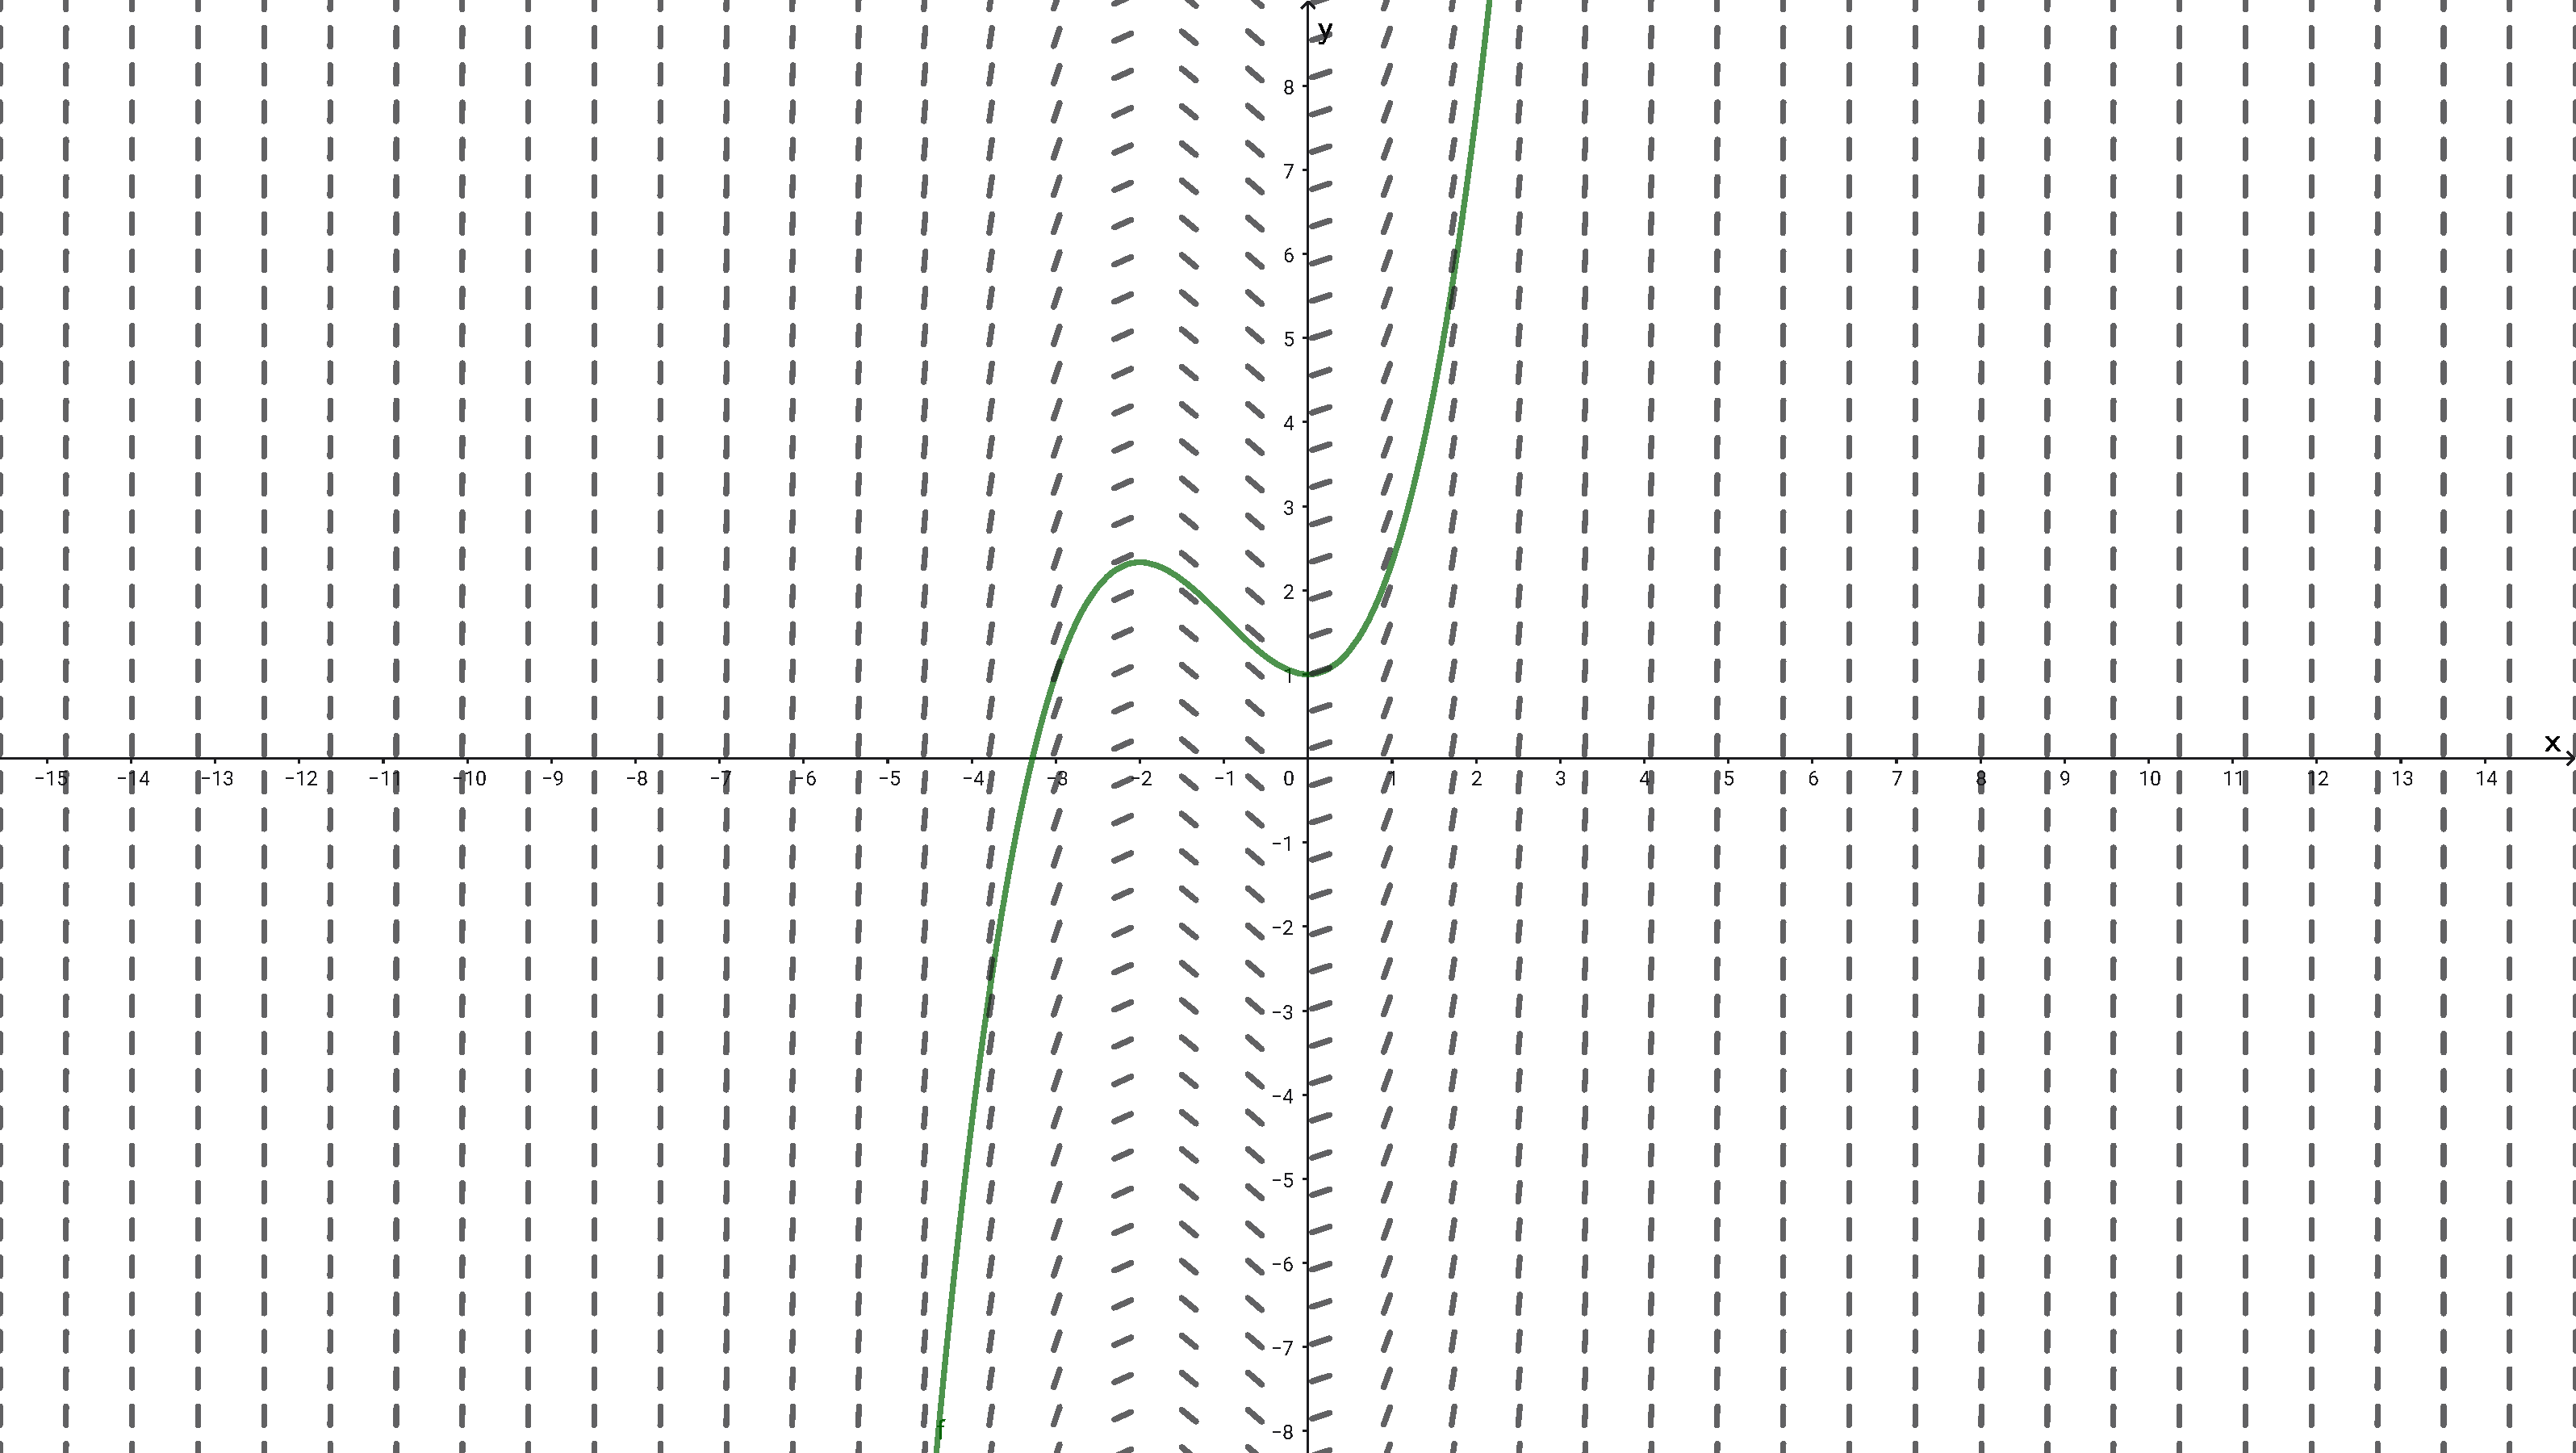
\includegraphics[width=0.72\textwidth]{img/unidad1_bloque1_ejercicio1.pdf}
    \caption{Bloque 1 — Ejercicio 1. Curva solución $y = x^3/3 + x^2 + c$ de la EDO $y' - x^2 - 2x = 0$.}
\end{figure}

\textbf{Ejercicio 2.} $y' = 3x^2$

\textit{Solución:}

\[
dy = 3x^2\,dx \implies \int dy = \int 3x^2\,dx \implies y = x^3
\]

Verificación: $y' = 3x^2$.
\[
\boxed{3x^2 = 3x^2 \quad \checkmark}
\]

\begin{figure}[H]
    \centering
    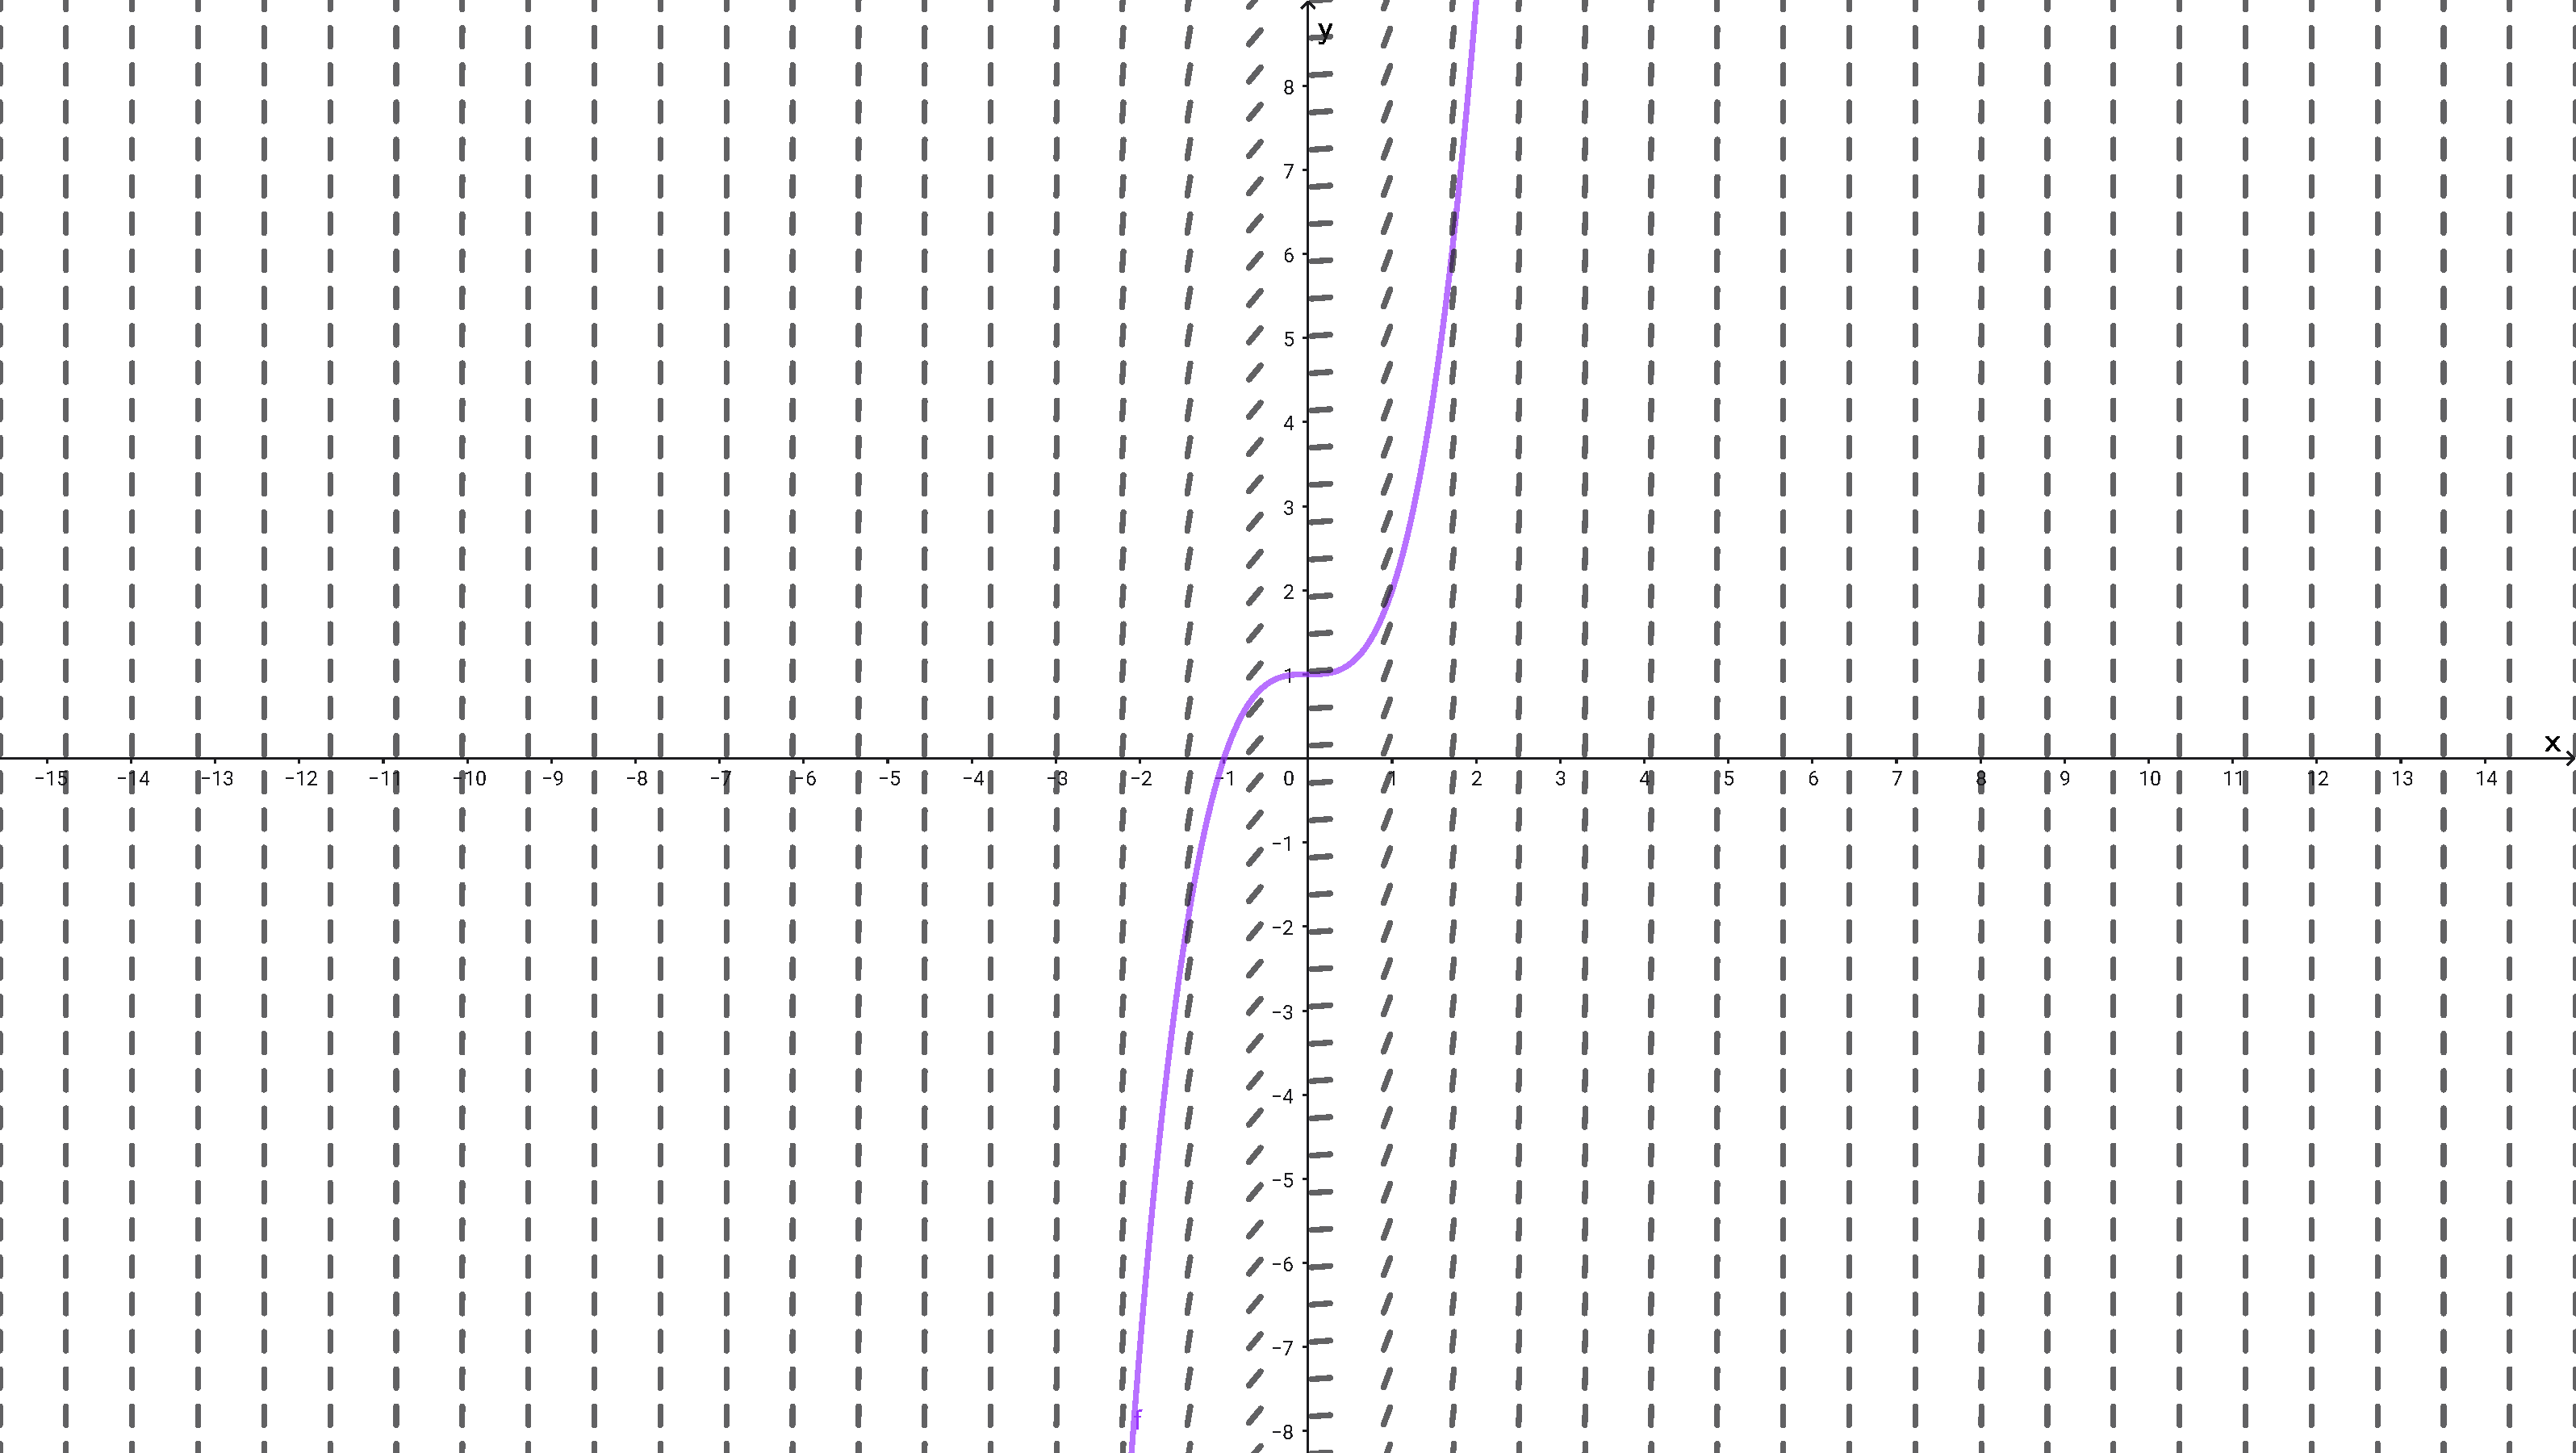
\includegraphics[width=0.72\textwidth]{img/unidad1_bloque1_ejercicio2.pdf}
    \caption{Bloque 1 — Ejercicio 2. Curva solución $y = x^3$ de la EDO $y' = 3x^2$.}
\end{figure}

\textbf{Ejercicio 3.} $y' = 2x^2 - 5$

\textit{Solución:}

\[
dy = (2x^2 - 5)\,dx \implies y = \dfrac{2x^3}{3} - 5x + c
\]

Verificación:
\[
y' = \dfrac{6x^2}{3} - 5 = 2x^2 - 5
\]
\[
\boxed{2x^2 - 5 = 2x^2 - 5 \quad \checkmark}
\]

\begin{figure}[H]
    \centering
    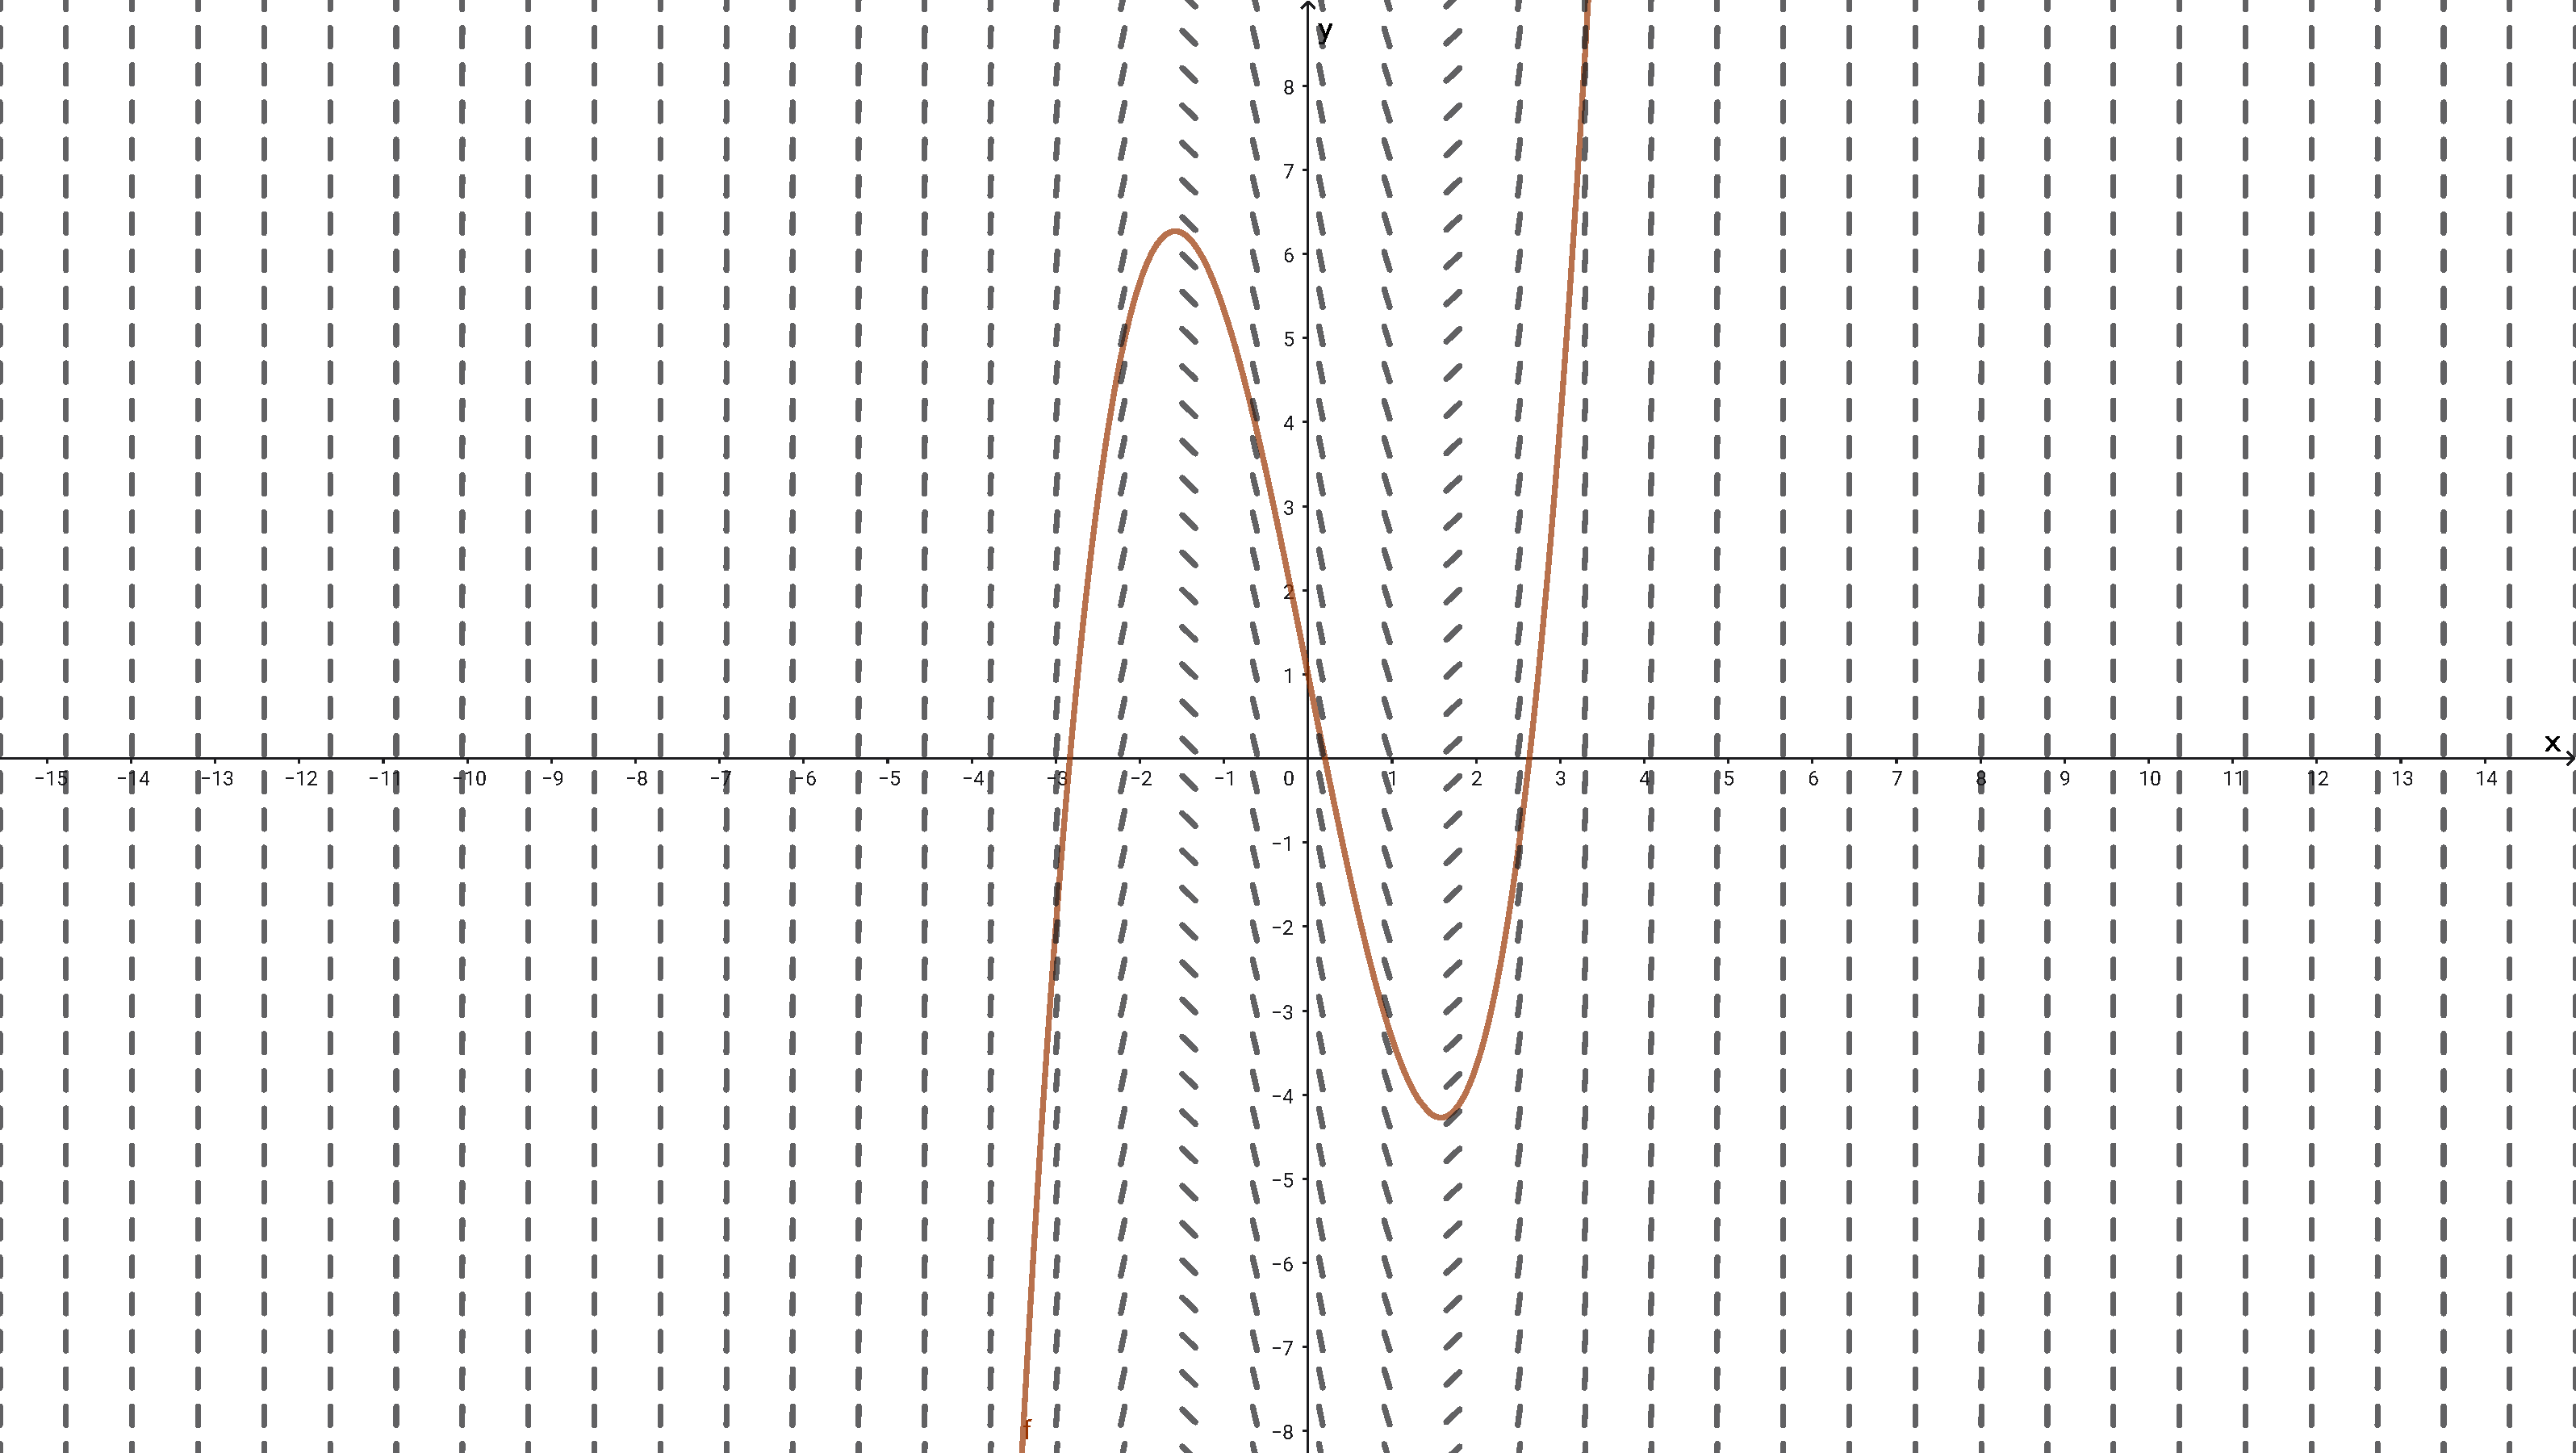
\includegraphics[width=0.72\textwidth]{img/unidad1_bloque1_ejercicio3.pdf}
    \caption{Bloque 1 — Ejercicio 3. Curva solución $y = 2x^3/3 - 5x + c$ de la EDO $y' = 2x^2 - 5$.}
\end{figure}

\textbf{Ejercicio 4.} $xy' = y$

\textit{Solución:}

Separando variables:
\[
\dfrac{dy}{y} = \dfrac{dx}{x} \implies \int \dfrac{dy}{y} = \int \dfrac{dx}{x} \implies \ln|y| = \ln|x| + c
\]
\[
y = x\,e^{c} = Cx
\]

Verificación: $y' = C$.
\[
x(C) = Cx \implies \boxed{Cx = Cx \quad \checkmark}
\]

\begin{figure}[H]
    \centering
    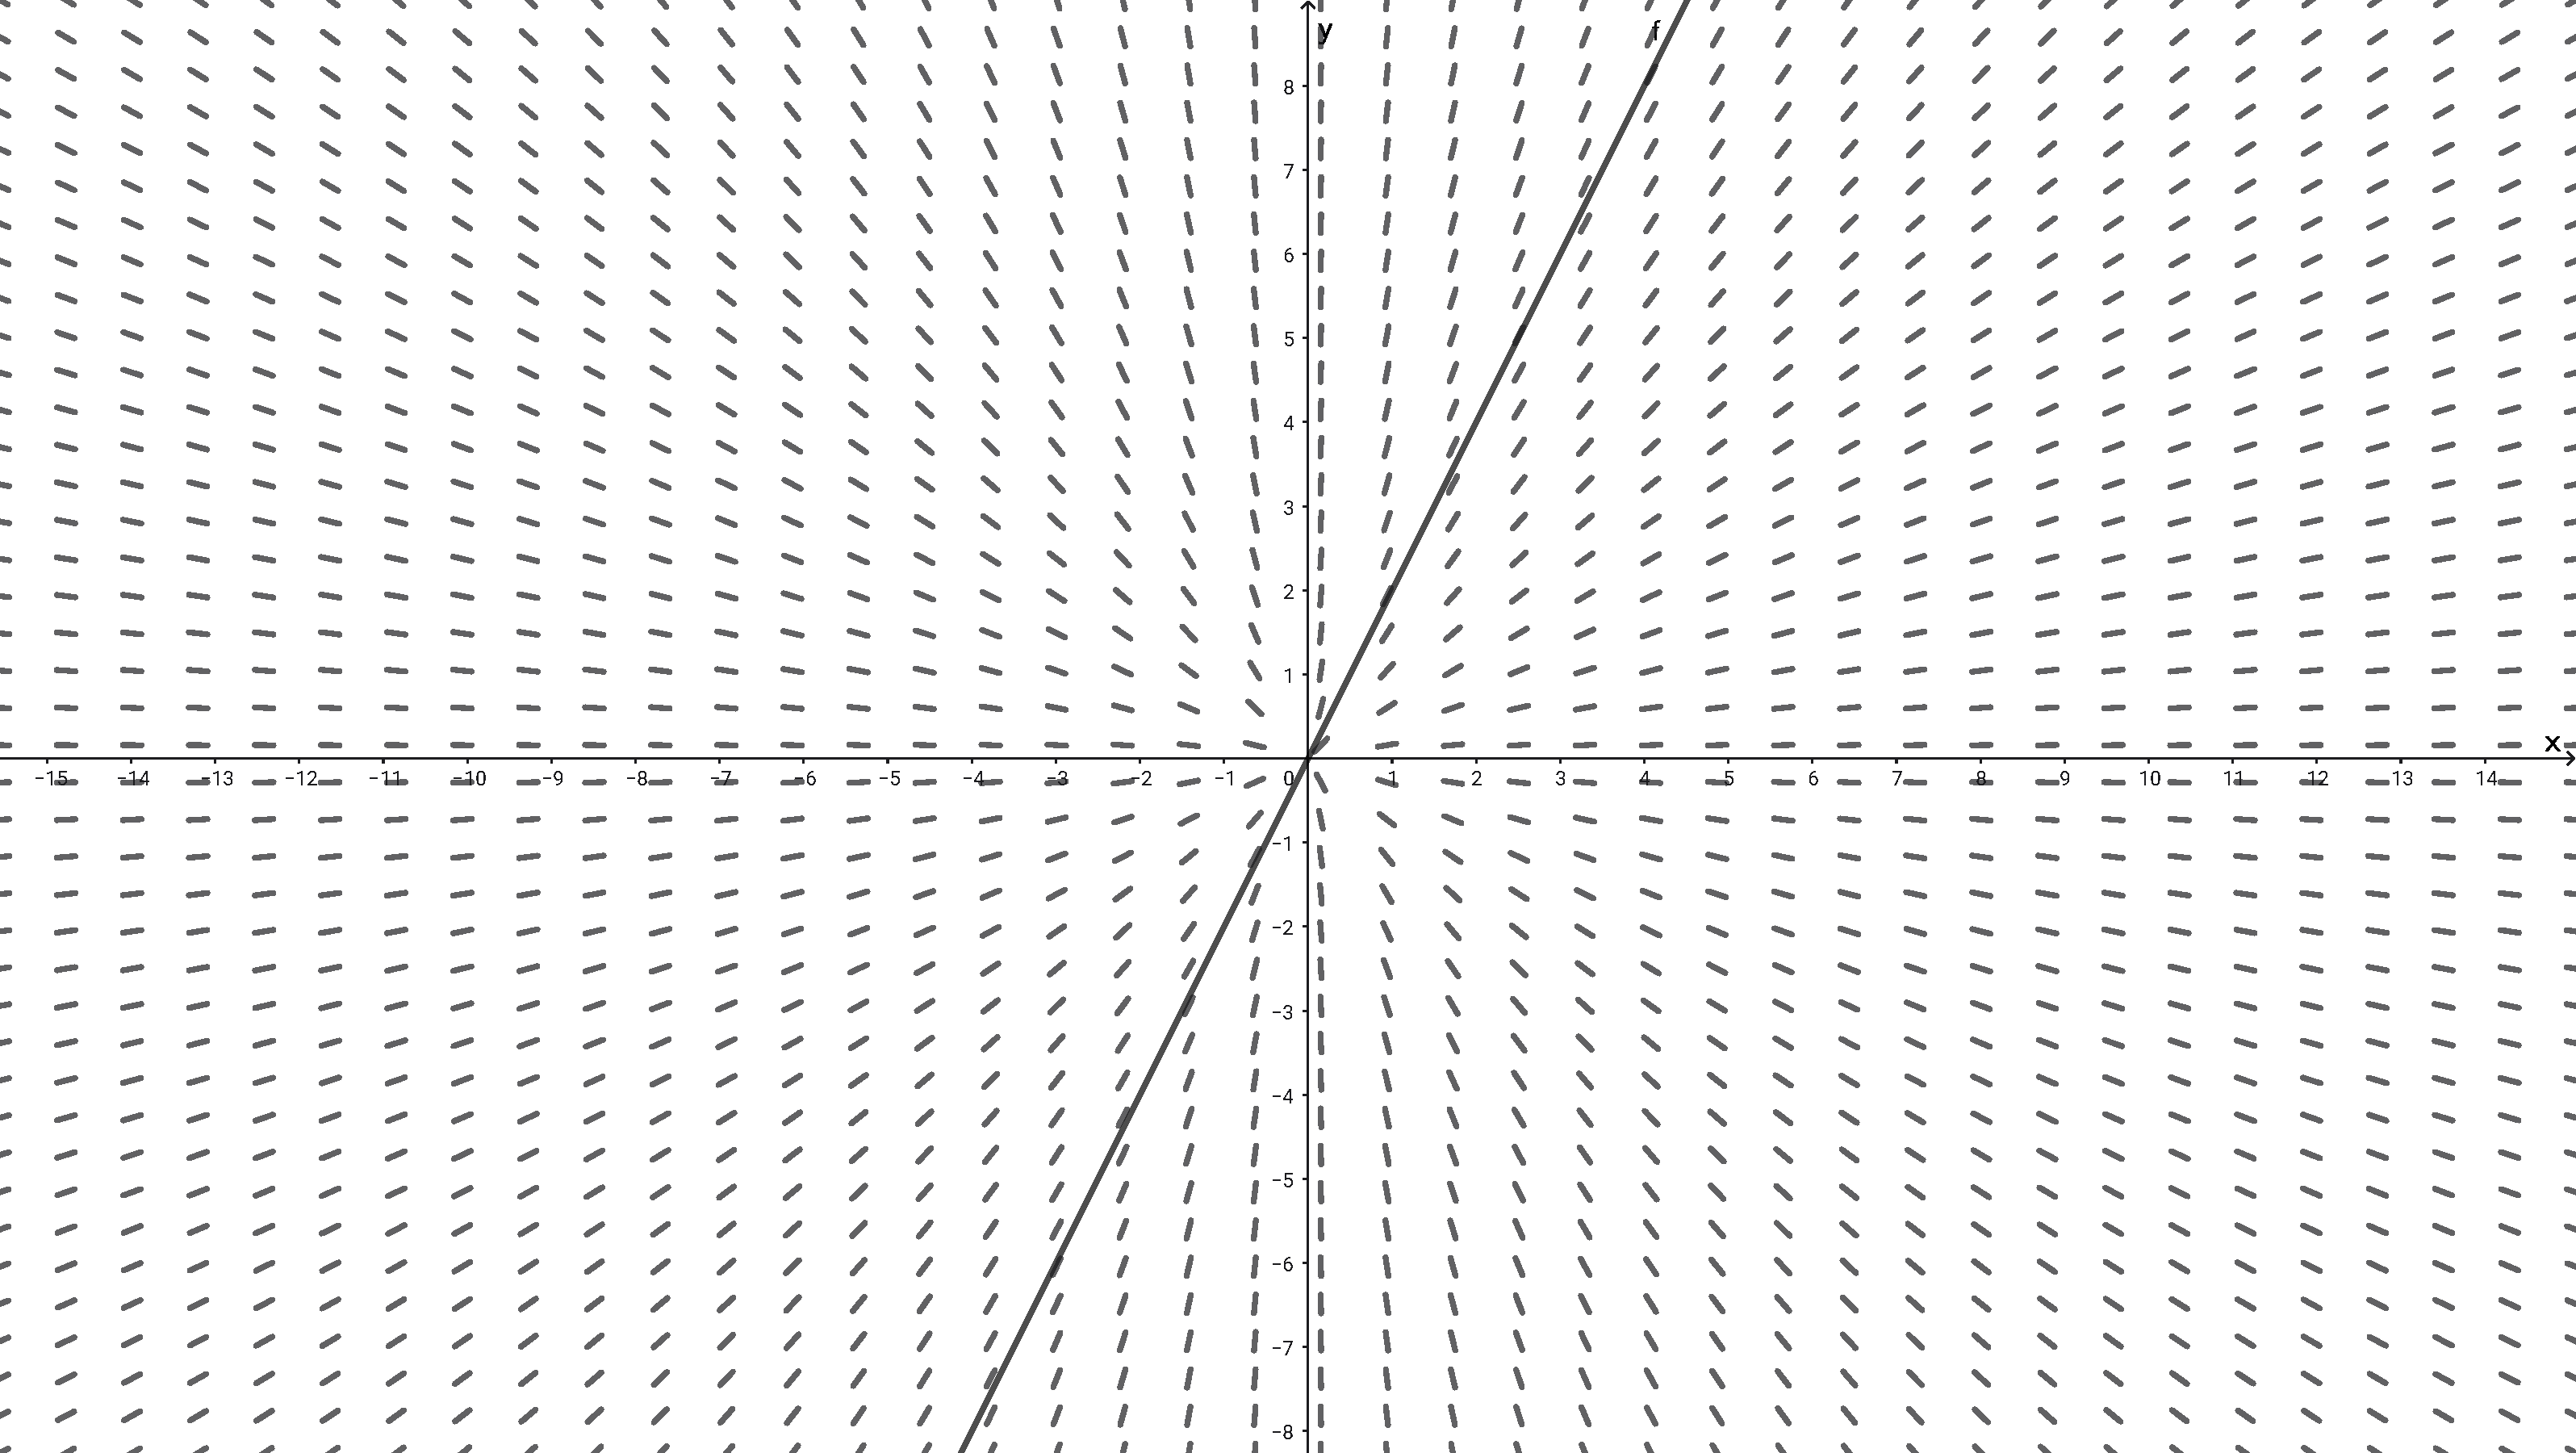
\includegraphics[width=0.72\textwidth]{img/unidad1_bloque1_ejercicio4.pdf}
    \caption{Bloque 1 — Ejercicio 4. Familia de soluciones $y = Cx$ de la EDO $xy' = y$.}
\end{figure}

\textbf{Ejercicio 5.} $y' + 4xy = 0$

\textit{Solución:}

\[
\dfrac{dy}{y} = -4x\,dx \implies \ln|y| = -2x^2 + c \implies y = C\,e^{-2x^2}
\]

Verificación: $y' = -4x\,C\,e^{-2x^2}$.
\[
-4x(C\,e^{-2x^2}) + 4x(C\,e^{-2x^2}) = 0 \implies \boxed{0 = 0 \quad \checkmark}
\]

\begin{figure}[H]
    \centering
    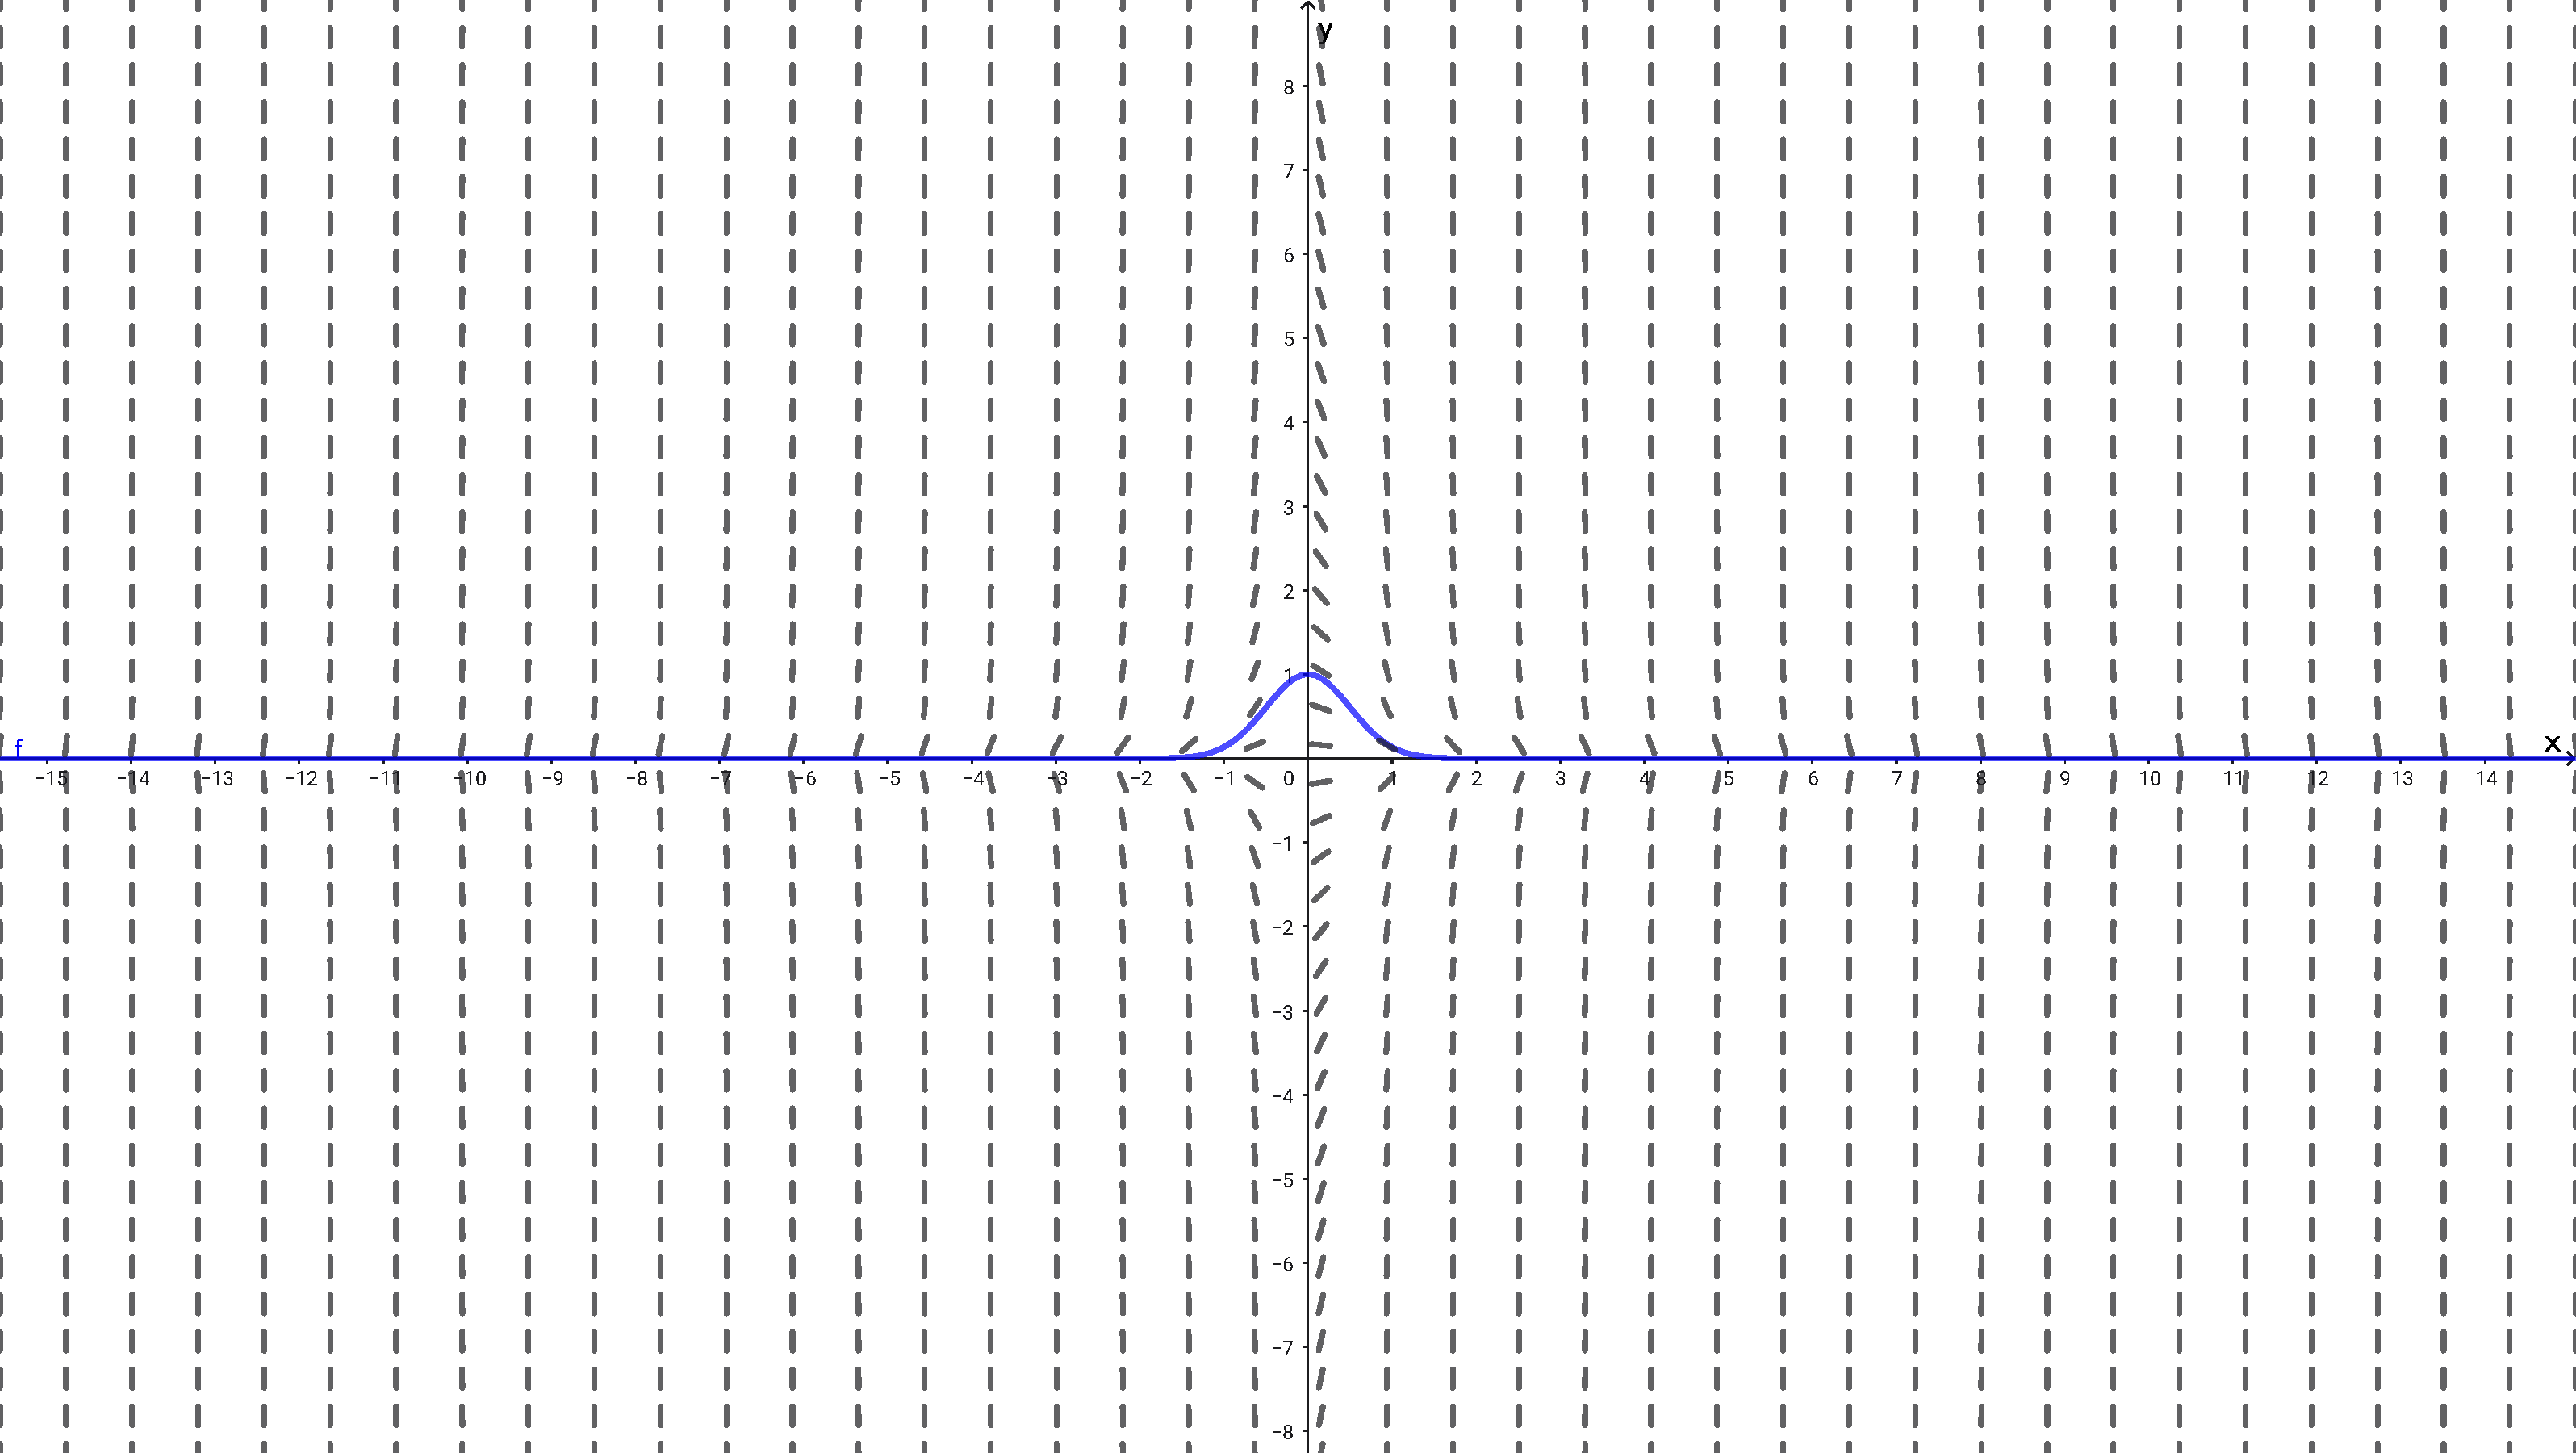
\includegraphics[width=0.72\textwidth]{img/unidad1_bloque1_ejercicio5.pdf}
    \caption{Bloque 1 — Ejercicio 5. Familia de soluciones $y = Ce^{-2x^2}$ de la EDO $y' + 4xy = 0$.}
\end{figure}

\textbf{Ejercicio 6.} $\dfrac{dy}{dx} = \dfrac{y\cos(x)}{1 - 2y}$

\textit{Solución:}

\[
\dfrac{1 - 2y}{y}\,dy = \cos(x)\,dx \implies \int\!\left(\dfrac{1}{y} - 2\right)dy = \int \cos(x)\,dx
\]
\[
\ln|y| - 2y = \sin(x) + c
\]

Verificación mediante diferenciación implícita:
\[
\dfrac{1}{y}\dfrac{dy}{dx} - 2\dfrac{dy}{dx} = \cos(x) \implies \dfrac{dy}{dx}\!\left(\dfrac{1}{y} - 2\right) = \cos(x)
\]
\[
\boxed{\dfrac{dy}{dx} = \dfrac{y\cos(x)}{1 - 2y} \quad \checkmark}
\]

\begin{figure}[H]
    \centering
    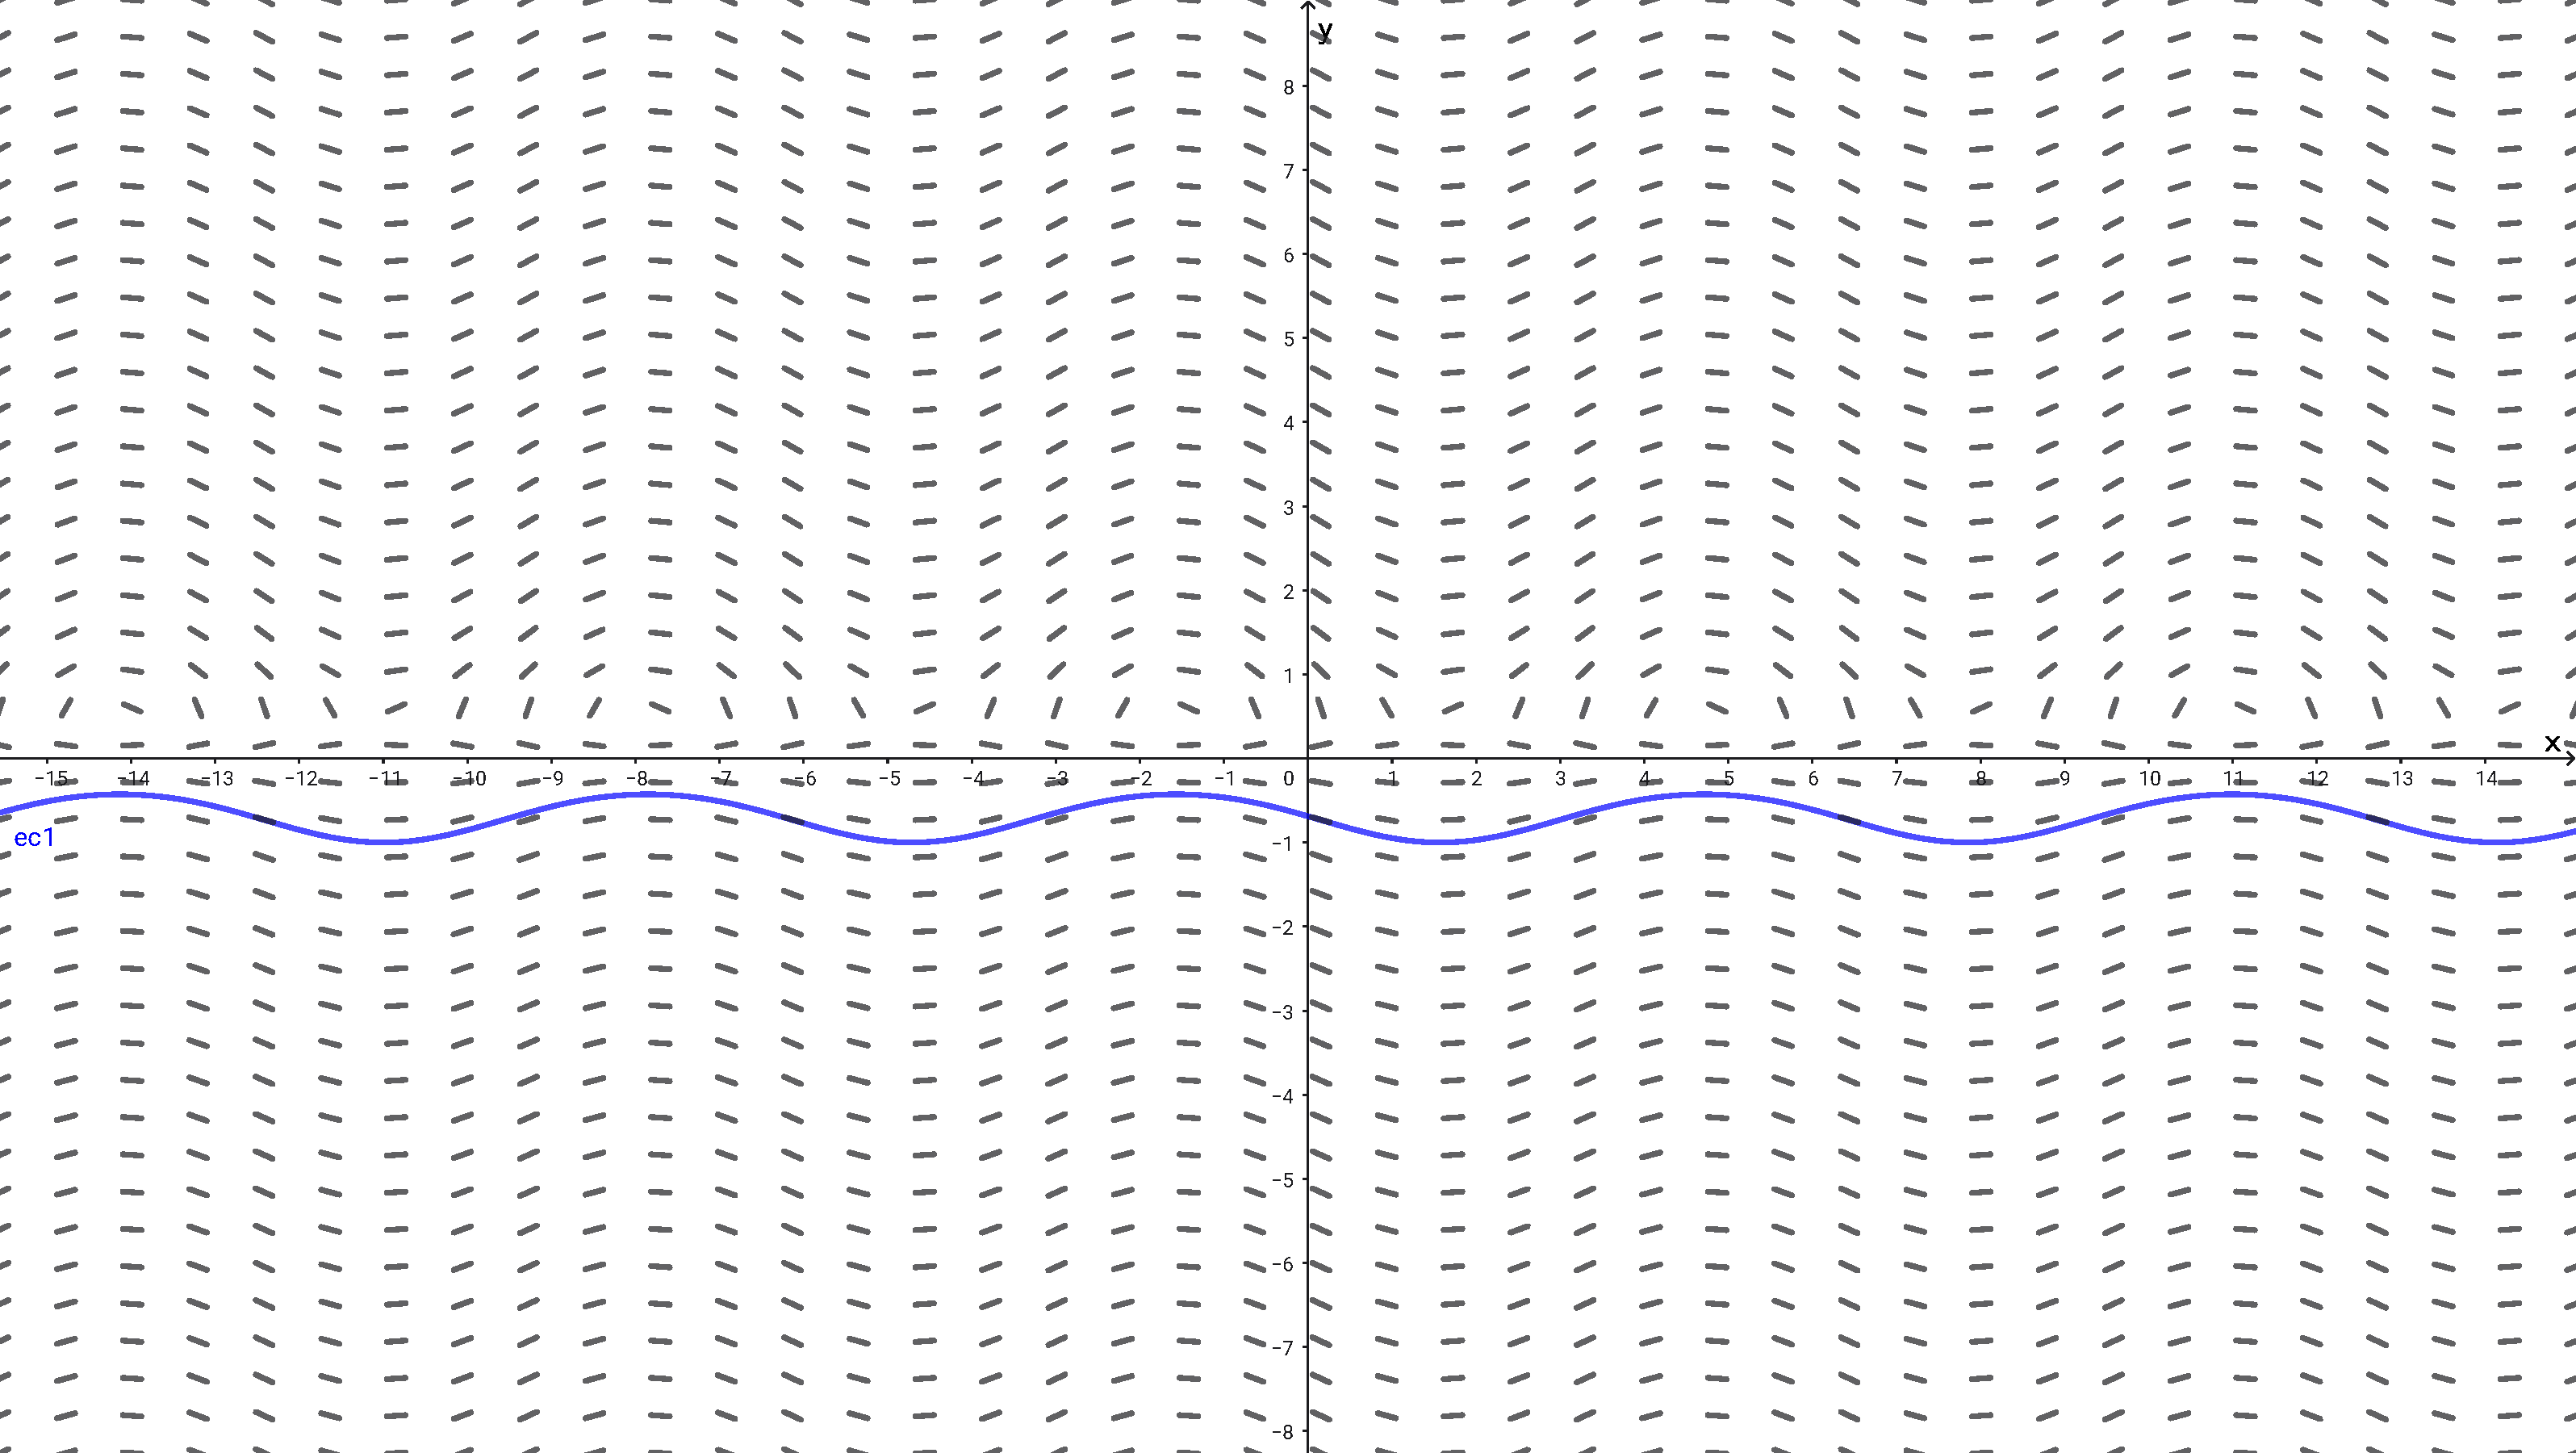
\includegraphics[width=0.72\textwidth]{img/unidad1_bloque1_ejercicio6.pdf}
    \caption{Bloque 1 — Ejercicio 6. Curvas de nivel de la solución implícita $\ln|y| - 2y = \sin(x) + c$ de la EDO $dy/dx = y\cos(x)/(1-2y)$.}
\end{figure}

\textbf{Ejercicio 7.} $\dfrac{dy}{dx} - e^{x+y} = 0$

\textit{Solución:}

\[
e^{-y}\,dy = e^{x}\,dx \implies \int e^{-y}\,dy = \int e^{x}\,dx \implies -e^{-y} = e^{x} + c
\]

Verificación implícita: derivando,
\[
e^{-y}\dfrac{dy}{dx} = e^{x} \implies \dfrac{dy}{dx} = \dfrac{e^{x}}{e^{-y}} = e^{x+y}
\]
\[
\boxed{e^{x+y} - e^{x+y} = 0 \quad \checkmark}
\]

\textbf{Ejercicio 8.} $y' \cdot y = \sin(x)$

\textit{Solución:}

\[
y\,dy = \sin(x)\,dx \implies \int y\,dy = \int \sin(x)\,dx \implies \dfrac{y^2}{2} = -\cos(x) + c
\]
\[
y^2 = c - 2\cos(x)
\]

Verificación: diferenciando implícitamente,
\[
2y\,y' = 2\sin(x) \implies y' = \dfrac{\sin(x)}{y}
\]
\[
\boxed{y\cdot\dfrac{\sin(x)}{y} = \sin(x) \quad \checkmark}
\]

\begin{figure}[H]
    \centering
    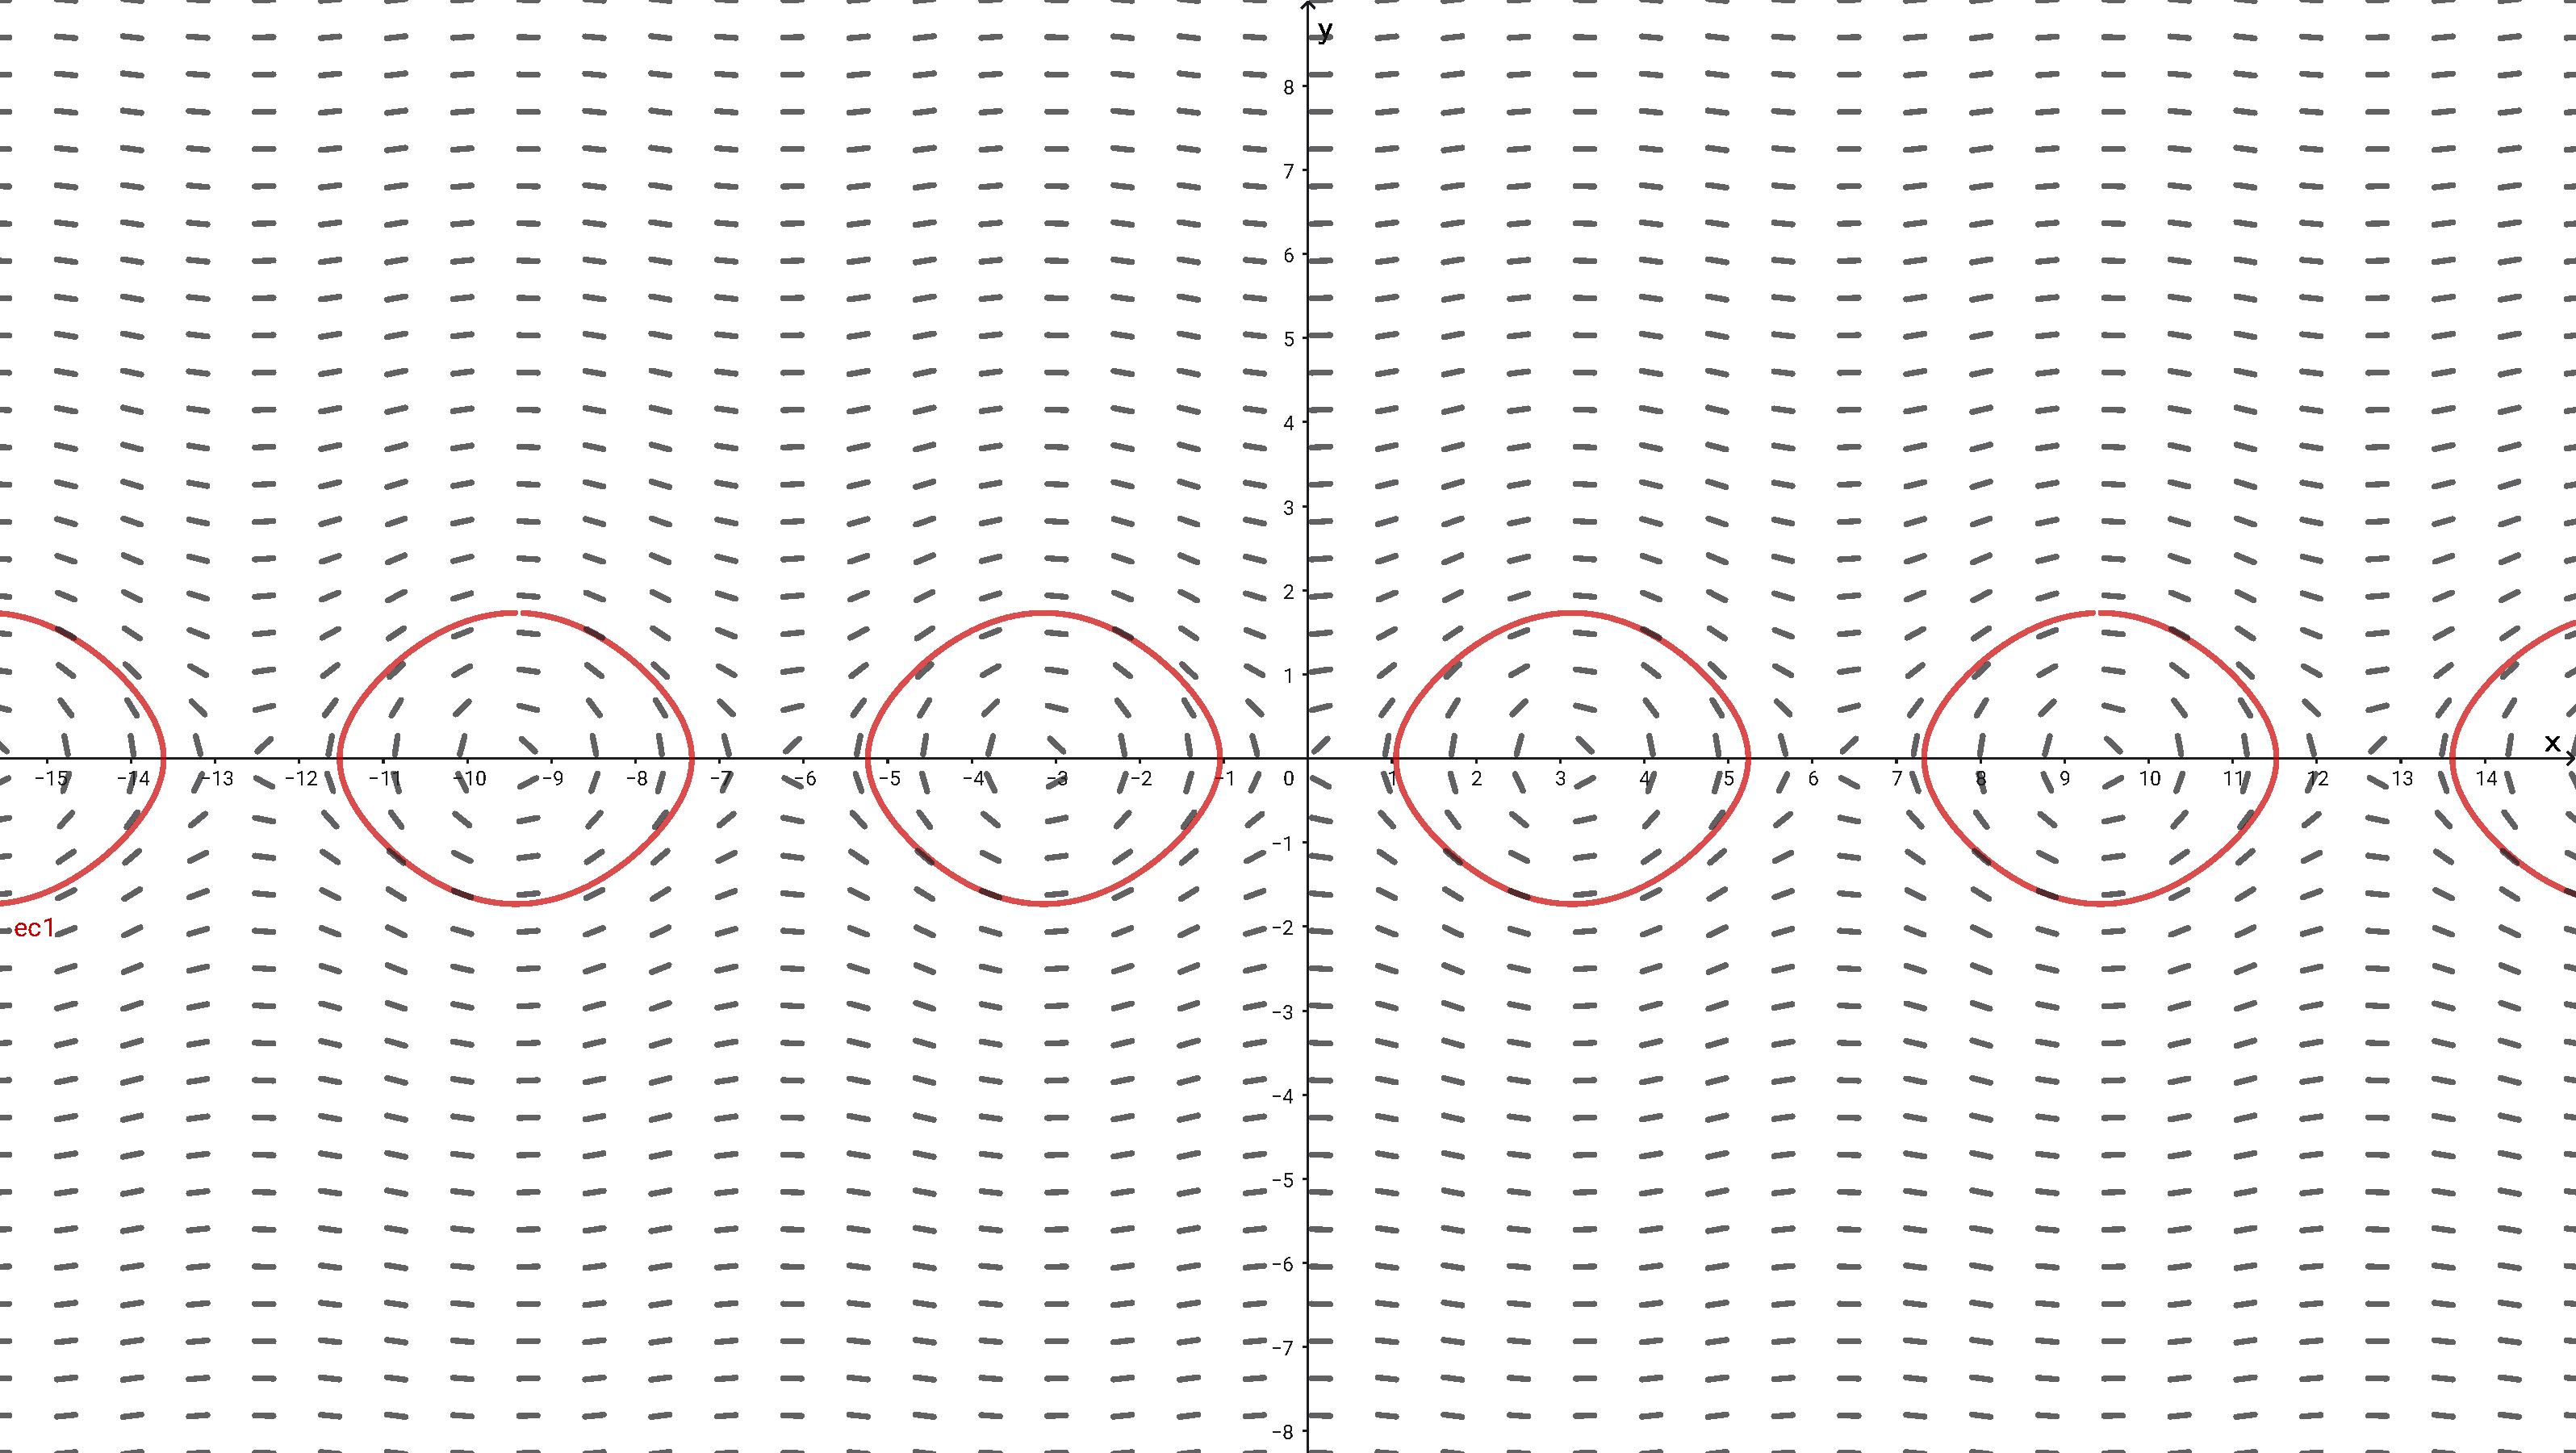
\includegraphics[width=0.72\textwidth]{img/unidad1_bloque1_ejercicio8.pdf}
    \caption{Bloque 1 — Ejercicio 8. Familia de curvas $y^2 = c - 2\cos(x)$ de la EDO $y' \cdot y = \sin(x)$.}
\end{figure}

\subsubsection*{Identificación de orden (Bloque 2)}

A continuación se clasifican ecuaciones por orden y naturaleza:

\begin{enumerate}
    \item $y'' - y = 2x$ \quad Ecuación diferencial de \textbf{2.º orden}.
    \item $y - 2x + 3y' = 0$ \quad Ecuación diferencial de \textbf{1.er orden}.
    \item $y - 3x = 0$ \quad Ecuación \textbf{algebraica}.
    \item $xy' - 2x = 5x$ \quad Ecuación diferencial de \textbf{1.er orden}.
    \item $\dfrac{d^3 y}{dx^3} + 4\dfrac{dy}{dx} + 3\dfrac{d^2 y}{dx^2} = 0$ \quad Ecuación diferencial de \textbf{3.er orden}.
\end{enumerate}

\textbf{Trabajo en clase:}

\begin{enumerate}
    \item $y'' - 3y' + 2x\,y''' = 0$ \quad \textbf{3.er orden}.
    \item $y'' - y' = \sin(x)$ \quad \textbf{2.º orden}.
    \item $t + 3t = y^3 + 2x$ \quad \textbf{1.er orden}.
    \item $\dfrac{d^4 t}{dx^4} + 8\!\left(\dfrac{dt}{dx}\right)^2 + 2t = e^{t}$ \quad \textbf{4.º orden}.
    \item $x''y^2 + x'y^3 = 2y + 3$ \quad \textbf{2.º orden}.
\end{enumerate}

% ============================================================

\section{Ecuaciones Diferenciales de Variables Separables}

\subsection{Metodología de Resolución y Separación de Diferenciales}

Una ecuación diferencial de primer orden es de \textbf{variables separables} cuando puede reescribirse de modo que todos los términos que involucran la variable dependiente $y$ queden de un lado del igual y todos los que involucran la variable independiente $x$ queden del otro. La forma canónica es:
\begin{equation*}
g(y)\,dy = f(x)\,dx
\end{equation*}

El procedimiento de resolución consta de tres etapas:

\begin{enumerate}
    \item \textbf{Separación algebraica}: manipular la ecuación hasta conseguir la forma $g(y)\,dy = f(x)\,dx$.
    \item \textbf{Integración}: aplicar $\displaystyle\int g(y)\,dy = \int f(x)\,dx$ en ambos miembros.
    \item \textbf{Despeje} (si es posible): expresar $y$ en función de $x$ de manera explícita.
\end{enumerate}

La técnica descansa en el supuesto de que $g(y) \neq 0$ en el dominio de análisis. Los puntos donde $g(y) = 0$ dan lugar a \textbf{soluciones singulares} que deben verificarse por separado.

\subsection{Ejercicios: Variables Separables (Bloque 3, parte 1)}

\textbf{Ejercicio 1.} $(2x + 1)y' = 3y$

\textit{Solución:}

\begin{align*}
\dfrac{dy}{y} &= \dfrac{3}{2x + 1}\,dx \\[4pt]
\int \dfrac{dy}{y} &= 3\int \dfrac{dx}{2x + 1} \\[4pt]
\ln|y| &= \dfrac{3}{2}\ln|2x + 1| + c \\[4pt]
y &= C(2x + 1)^{3/2}
\end{align*}

Verificación: $y' = C\cdot\dfrac{3}{2}(2x + 1)^{1/2}\cdot 2 = 3C(2x + 1)^{1/2}$.
\[
(2x + 1)\cdot 3C(2x + 1)^{1/2} = 3C(2x + 1)^{3/2}
\]
\[
\boxed{3C(2x+1)^{3/2} = 3C(2x+1)^{3/2} \quad \checkmark}
\]

\begin{figure}[H]
    \centering
    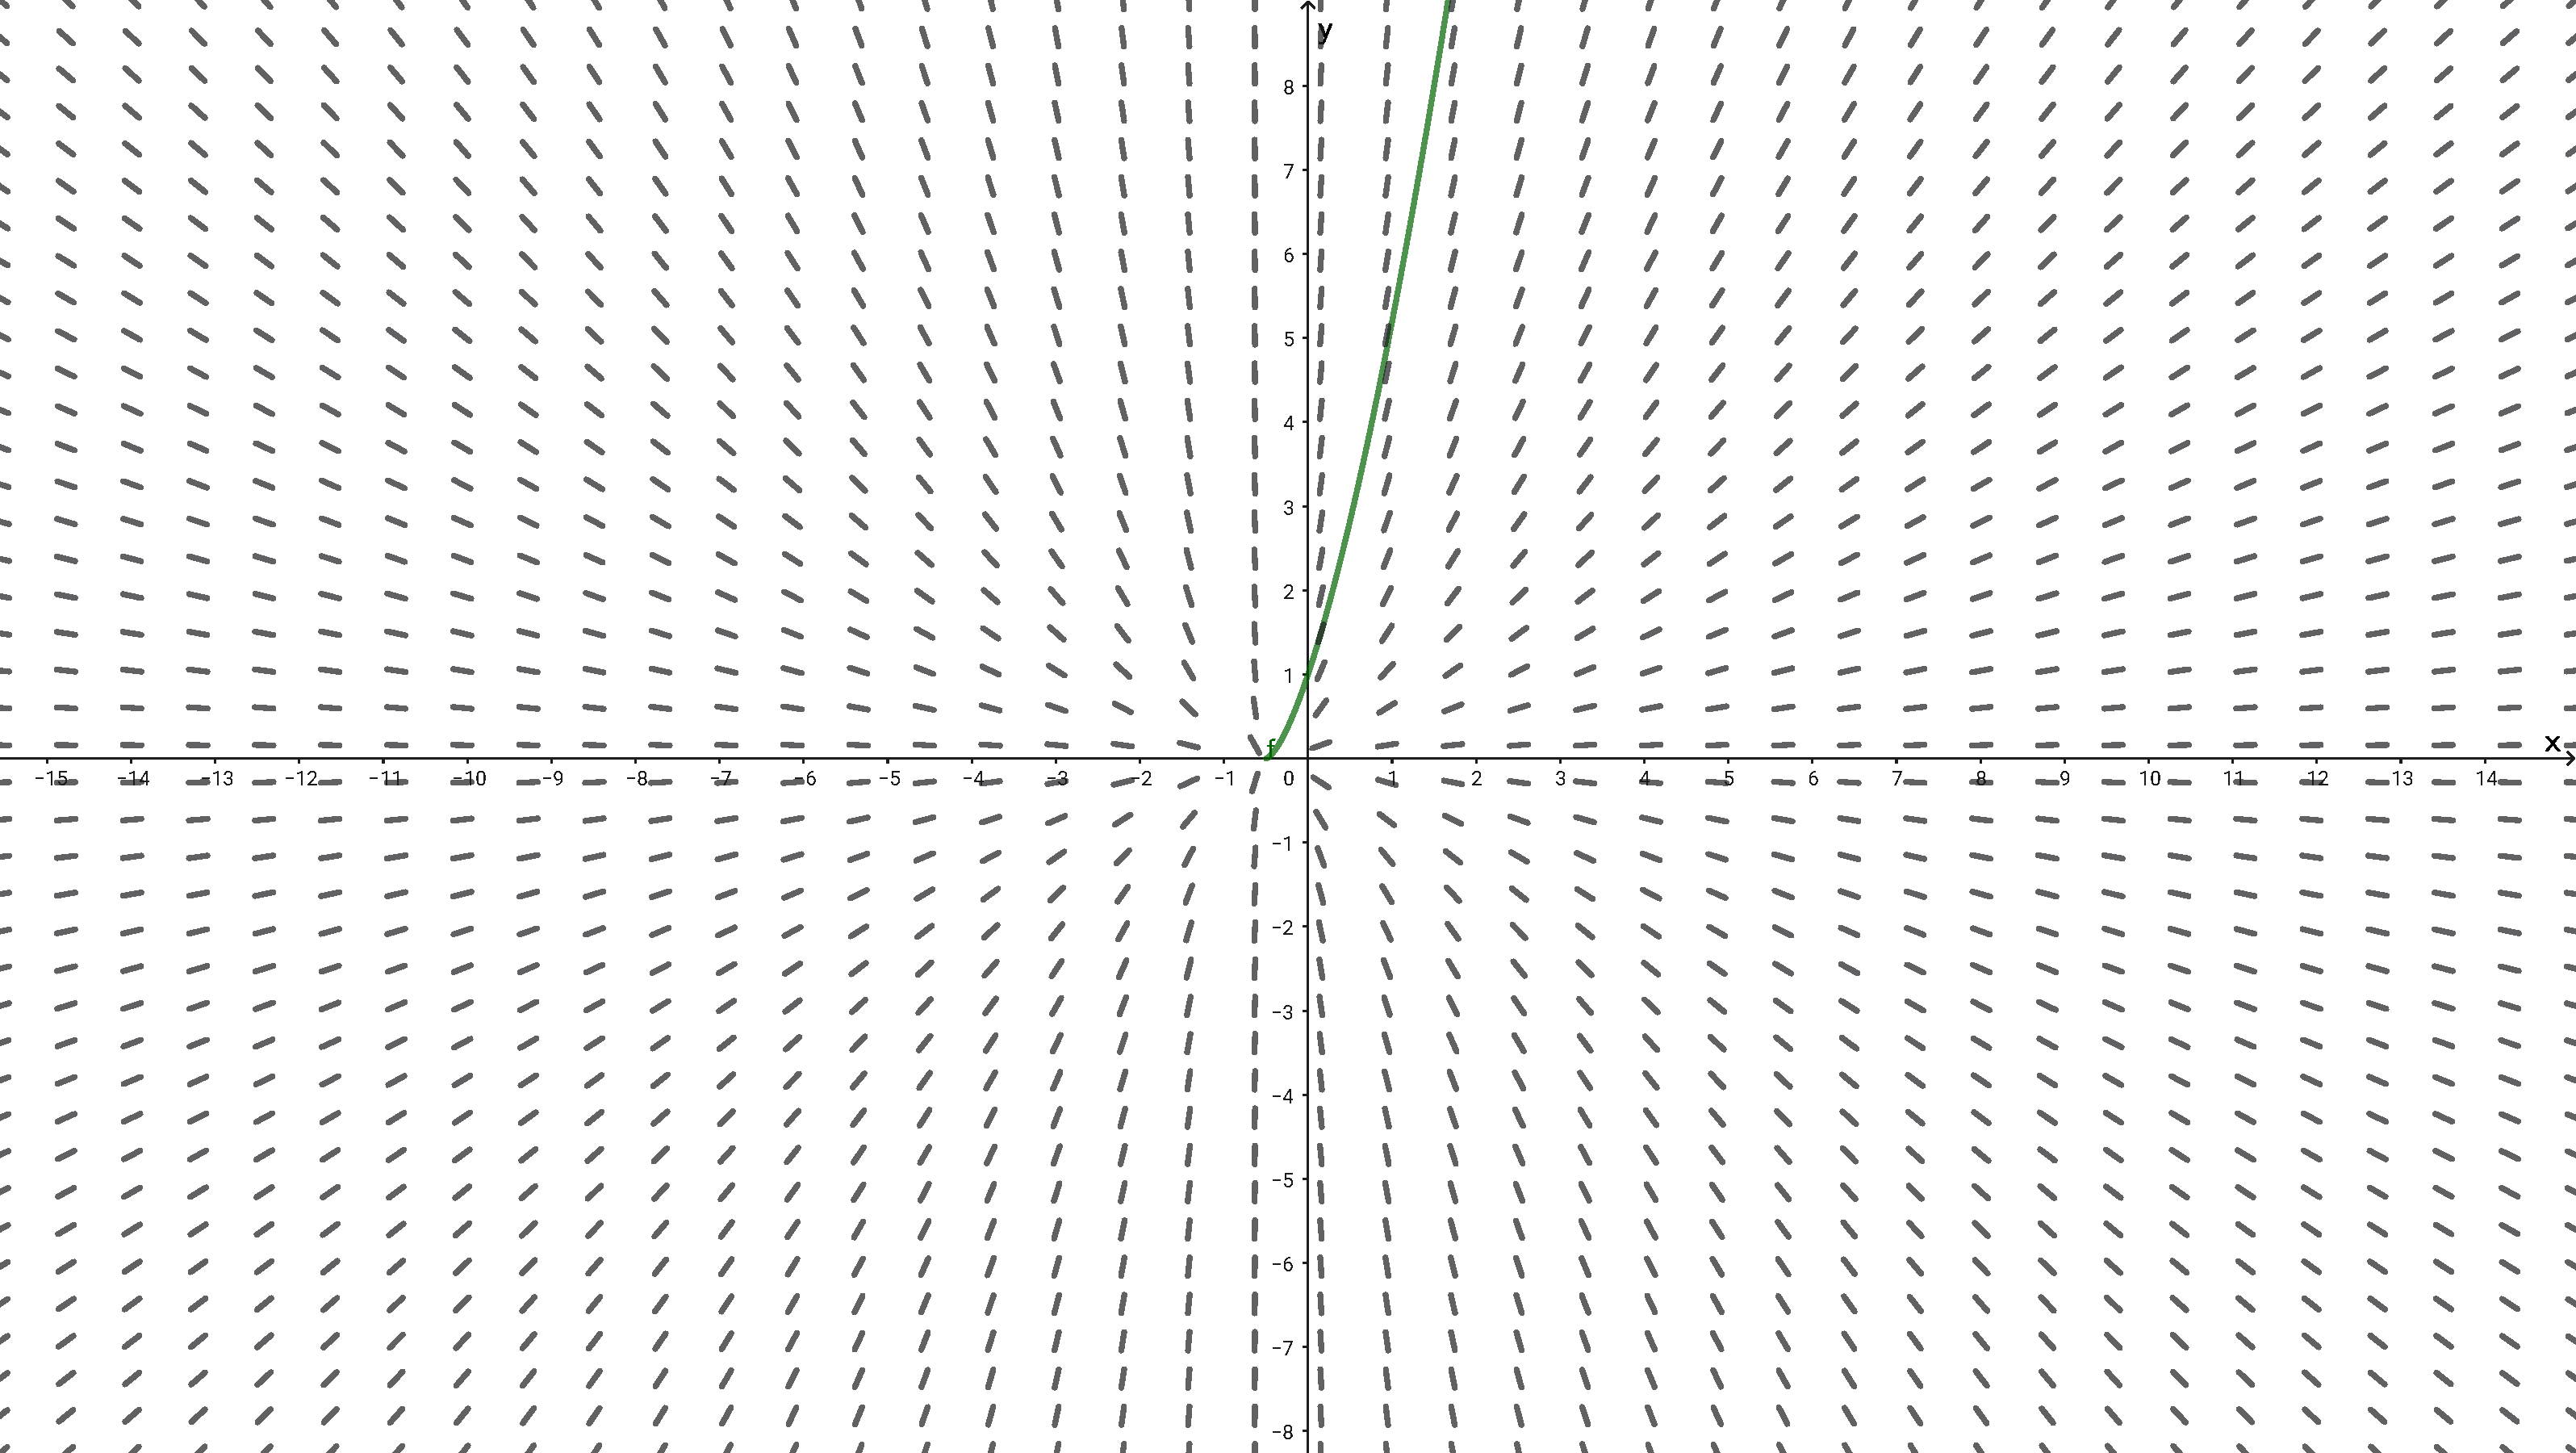
\includegraphics[width=0.72\textwidth]{img/unidad1_bloque3_ejercicio1.pdf}
    \caption{Bloque 3 — Ejercicio 1. Familia de curvas $y = C(2x+1)^{3/2}$ de la EDO de variables separables $(2x+1)y' = 3y$.}
\end{figure}

\textbf{Ejercicio 2.} $x\sin(y) + (x^2 + 1)\cos(y)\,y' = 0$

\textit{Solución:}

\begin{align*}
(x^2 + 1)\cos(y)\dfrac{dy}{dx} &= -x\sin(y) \\[4pt]
\dfrac{\cos(y)}{\sin(y)}\,dy &= -\dfrac{x}{x^2 + 1}\,dx \\[4pt]
\int \cot(y)\,dy &= -\int \dfrac{x}{x^2 + 1}\,dx \\[4pt]
\ln|\sin(y)| &= -\dfrac{1}{2}\ln(x^2 + 1) + c
\end{align*}
\[
\sin(y) = \dfrac{C}{(x^2 + 1)^{1/2}}
\]

Verificación implícita: diferenciando,
\[
\cos(y)\,y' = -Cx(x^2 + 1)^{-3/2}
\]

Sustituyendo en la ecuación original se verifica la identidad $0 = 0$. \quad $\checkmark$

\begin{figure}[H]
    \centering
    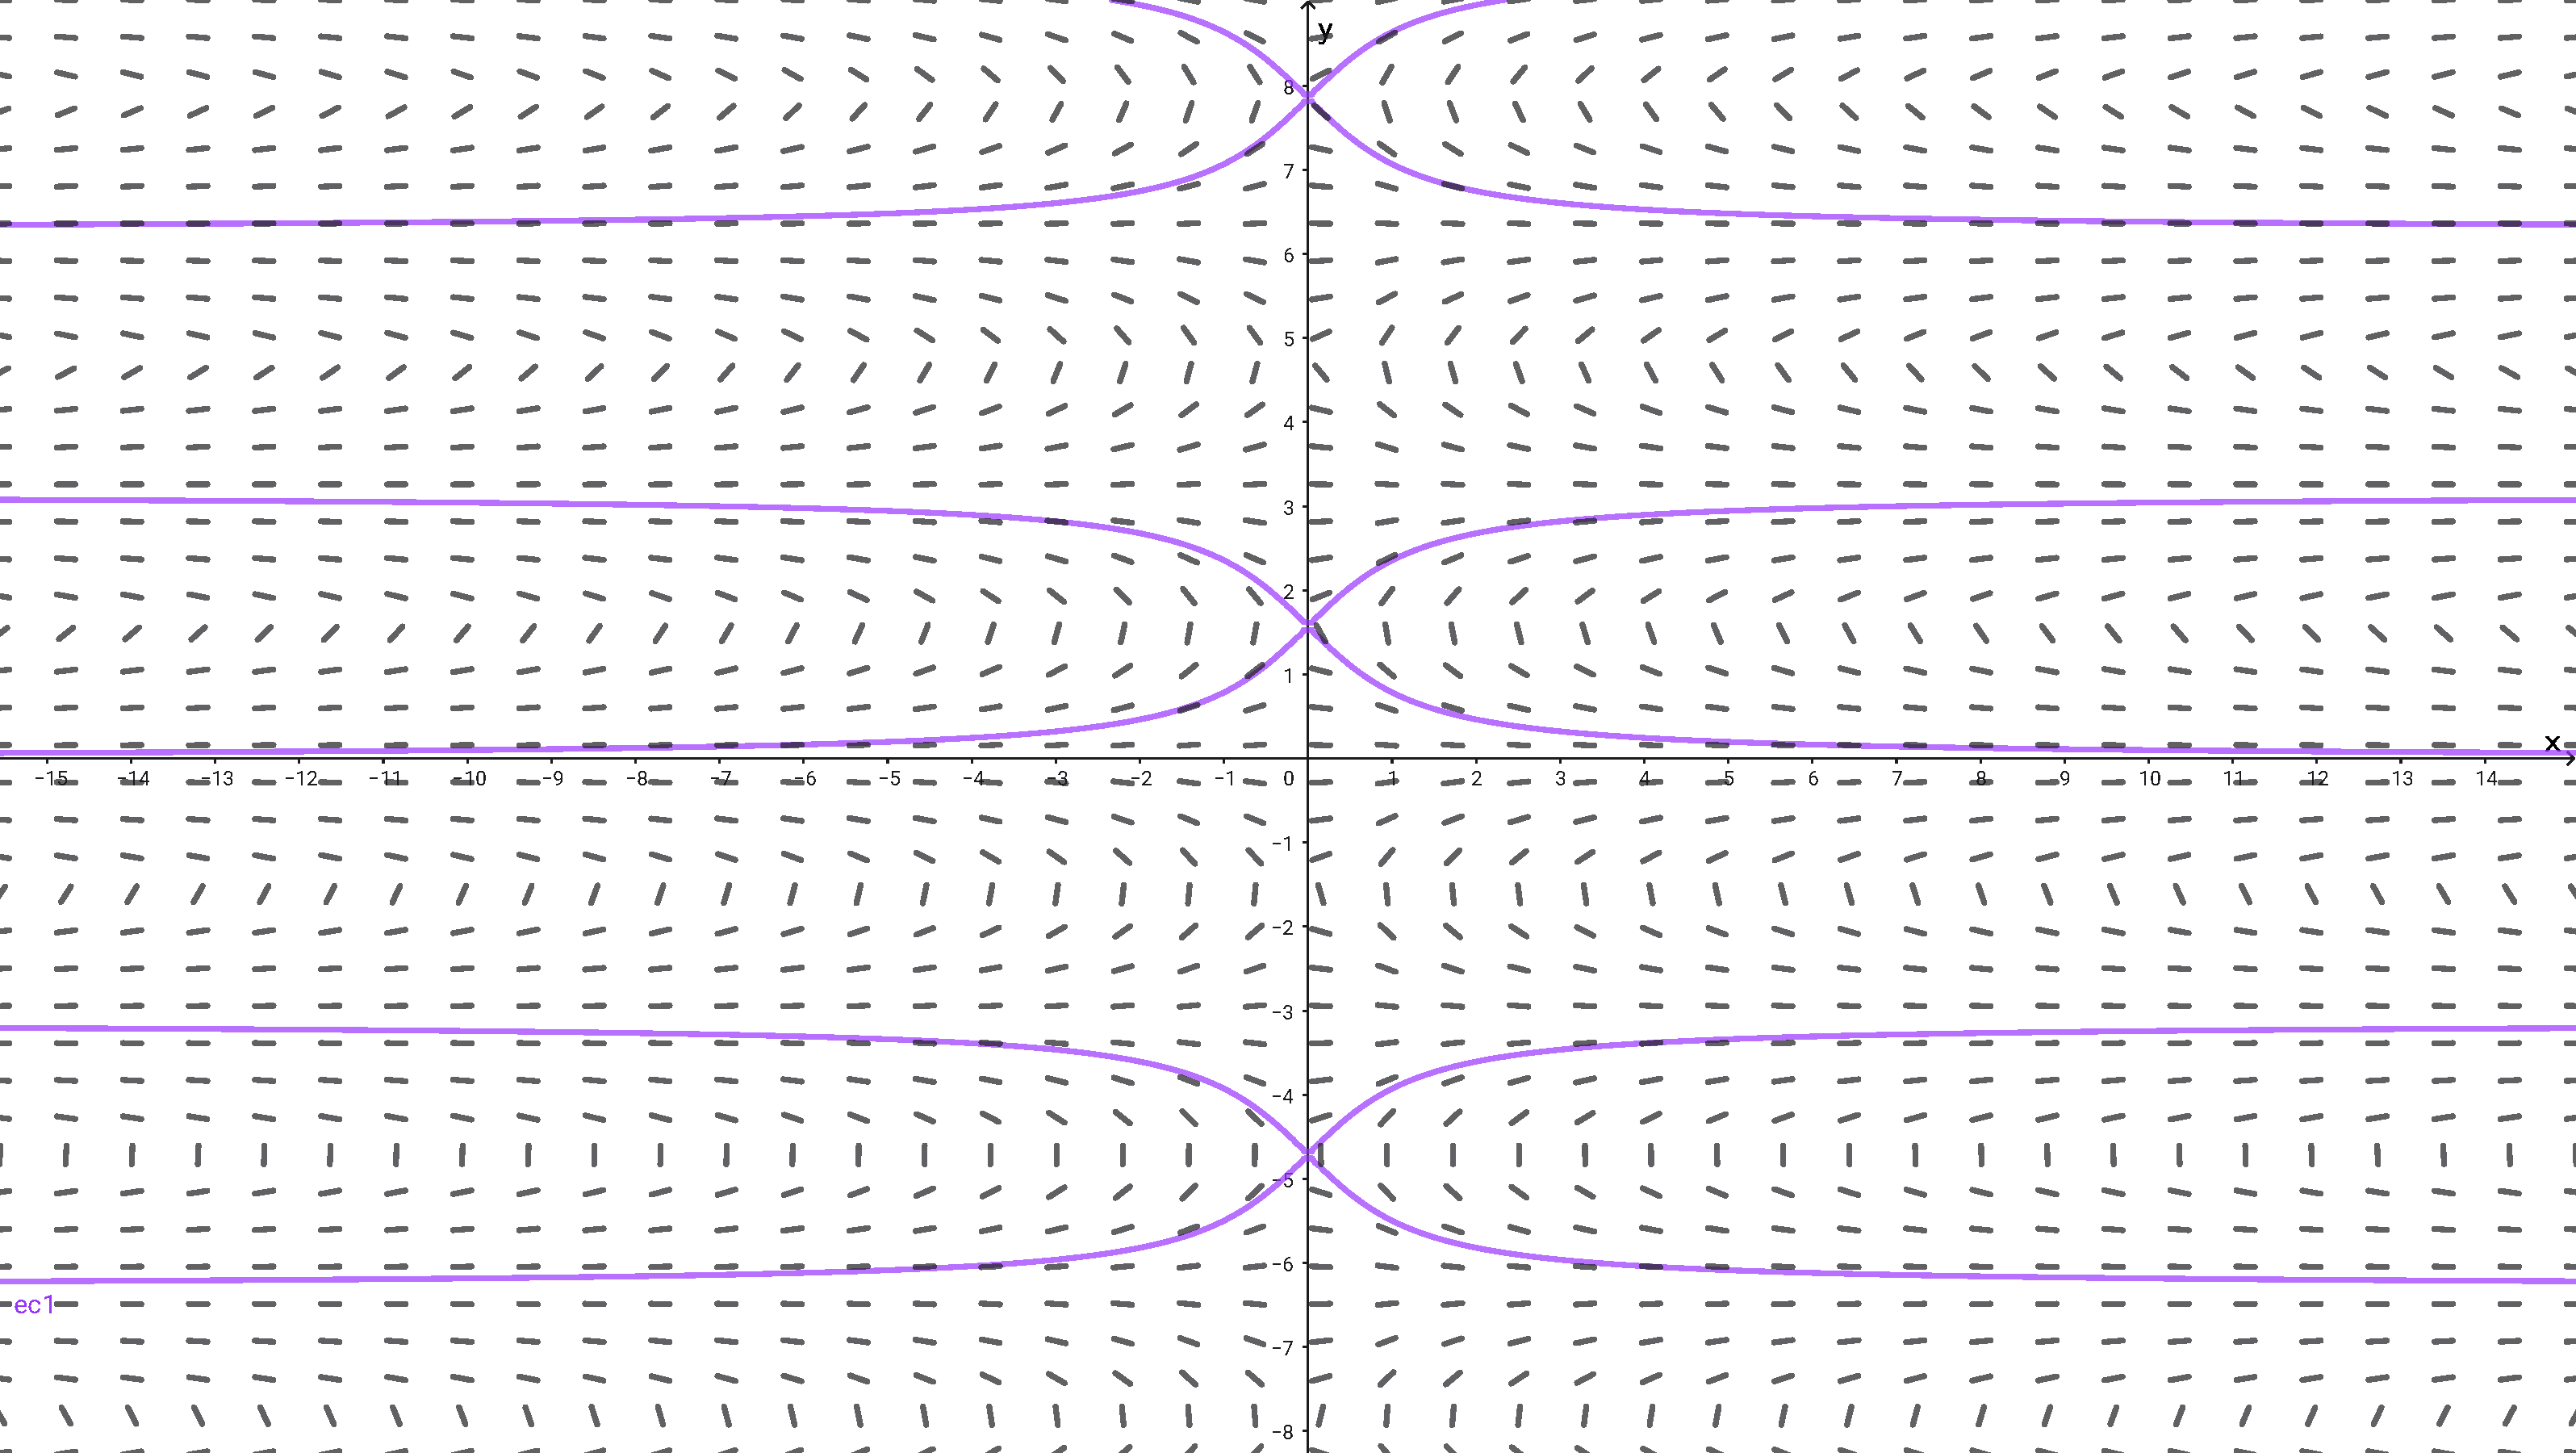
\includegraphics[width=0.72\textwidth]{img/unidad1_bloque3_ejercicio2.pdf}
    \caption{Bloque 3 — Ejercicio 2. Curvas de nivel de la solución implícita $\sin(y) = C(x^2+1)^{-1/2}$ de la EDO $x\sin(y) + (x^2+1)\cos(y)\,y' = 0$.}
\end{figure}

% ============================================================

\section{Ecuaciones Diferenciales Homogéneas}

\subsection{Definición y Función Homogénea de Grado Cero}

Una función $f(x,y)$ es \textbf{homogénea de grado} $k$ si para todo escalar $\lambda > 0$ se cumple:
\begin{equation*}
f(\lambda x,\, \lambda y) = \lambda^k f(x,y)
\end{equation*}

Una ecuación diferencial ordinaria de primer orden se denomina \textbf{homogénea} cuando puede expresarse en la forma:
\begin{equation*}
\dfrac{dy}{dx} = F\!\left(\dfrac{y}{x}\right)
\end{equation*}

es decir, cuando el cociente $\dfrac{dy}{dx}$ depende únicamente de la razón $y/x$. Esto ocurre cuando $M(x,y)$ y $N(x,y)$ en $M\,dx + N\,dy = 0$ son ambas homogéneas del mismo grado.

\subsection{Sustitución Algebraica $y = ux$}

El método de resolución consiste en introducir la sustitución $y = ux$, donde $u = u(x)$ es una nueva función incógnita. La diferencial es:
\[
dy = u\,dx + x\,du
\]

Al sustituir en la ecuación homogénea, el cociente $y/x$ se reemplaza por $u$, y la ecuación resultante es siempre de variables separables en $u$ y $x$. Una vez resuelta para $u(x)$, se revierte la sustitución escribiendo $u = y/x$.

\subsection{Ejercicios: Ecuaciones Homogéneas (Bloque 3, parte 2)}

\textbf{Ejercicio 3.} $\dfrac{dy}{dx} = \dfrac{x^2 + y^2}{xy}$

\textit{Solución:}

Verificación de homogeneidad: $M = -(x^2 + y^2)$, $N = xy$, ambas de grado 2. Sustitución $y = ux$, $dy = u\,dx + x\,du$:

\begin{align*}
u + x\dfrac{du}{dx} &= \dfrac{x^2 + u^2 x^2}{x \cdot ux} = \dfrac{1 + u^2}{u} \\[4pt]
x\dfrac{du}{dx} &= \dfrac{1 + u^2}{u} - u = \dfrac{1}{u}
\end{align*}

Separando:
\[
u\,du = \dfrac{dx}{x} \implies \int u\,du = \int \dfrac{dx}{x} \implies \dfrac{u^2}{2} = \ln|x| + c
\]

Revirtiendo $u = y/x$:
\[
\dfrac{y^2}{2x^2} = \ln|x| + c \implies \boxed{y^2 = 2x^2\ln|x| + Cx^2}
\]

\begin{figure}[H]
    \centering
    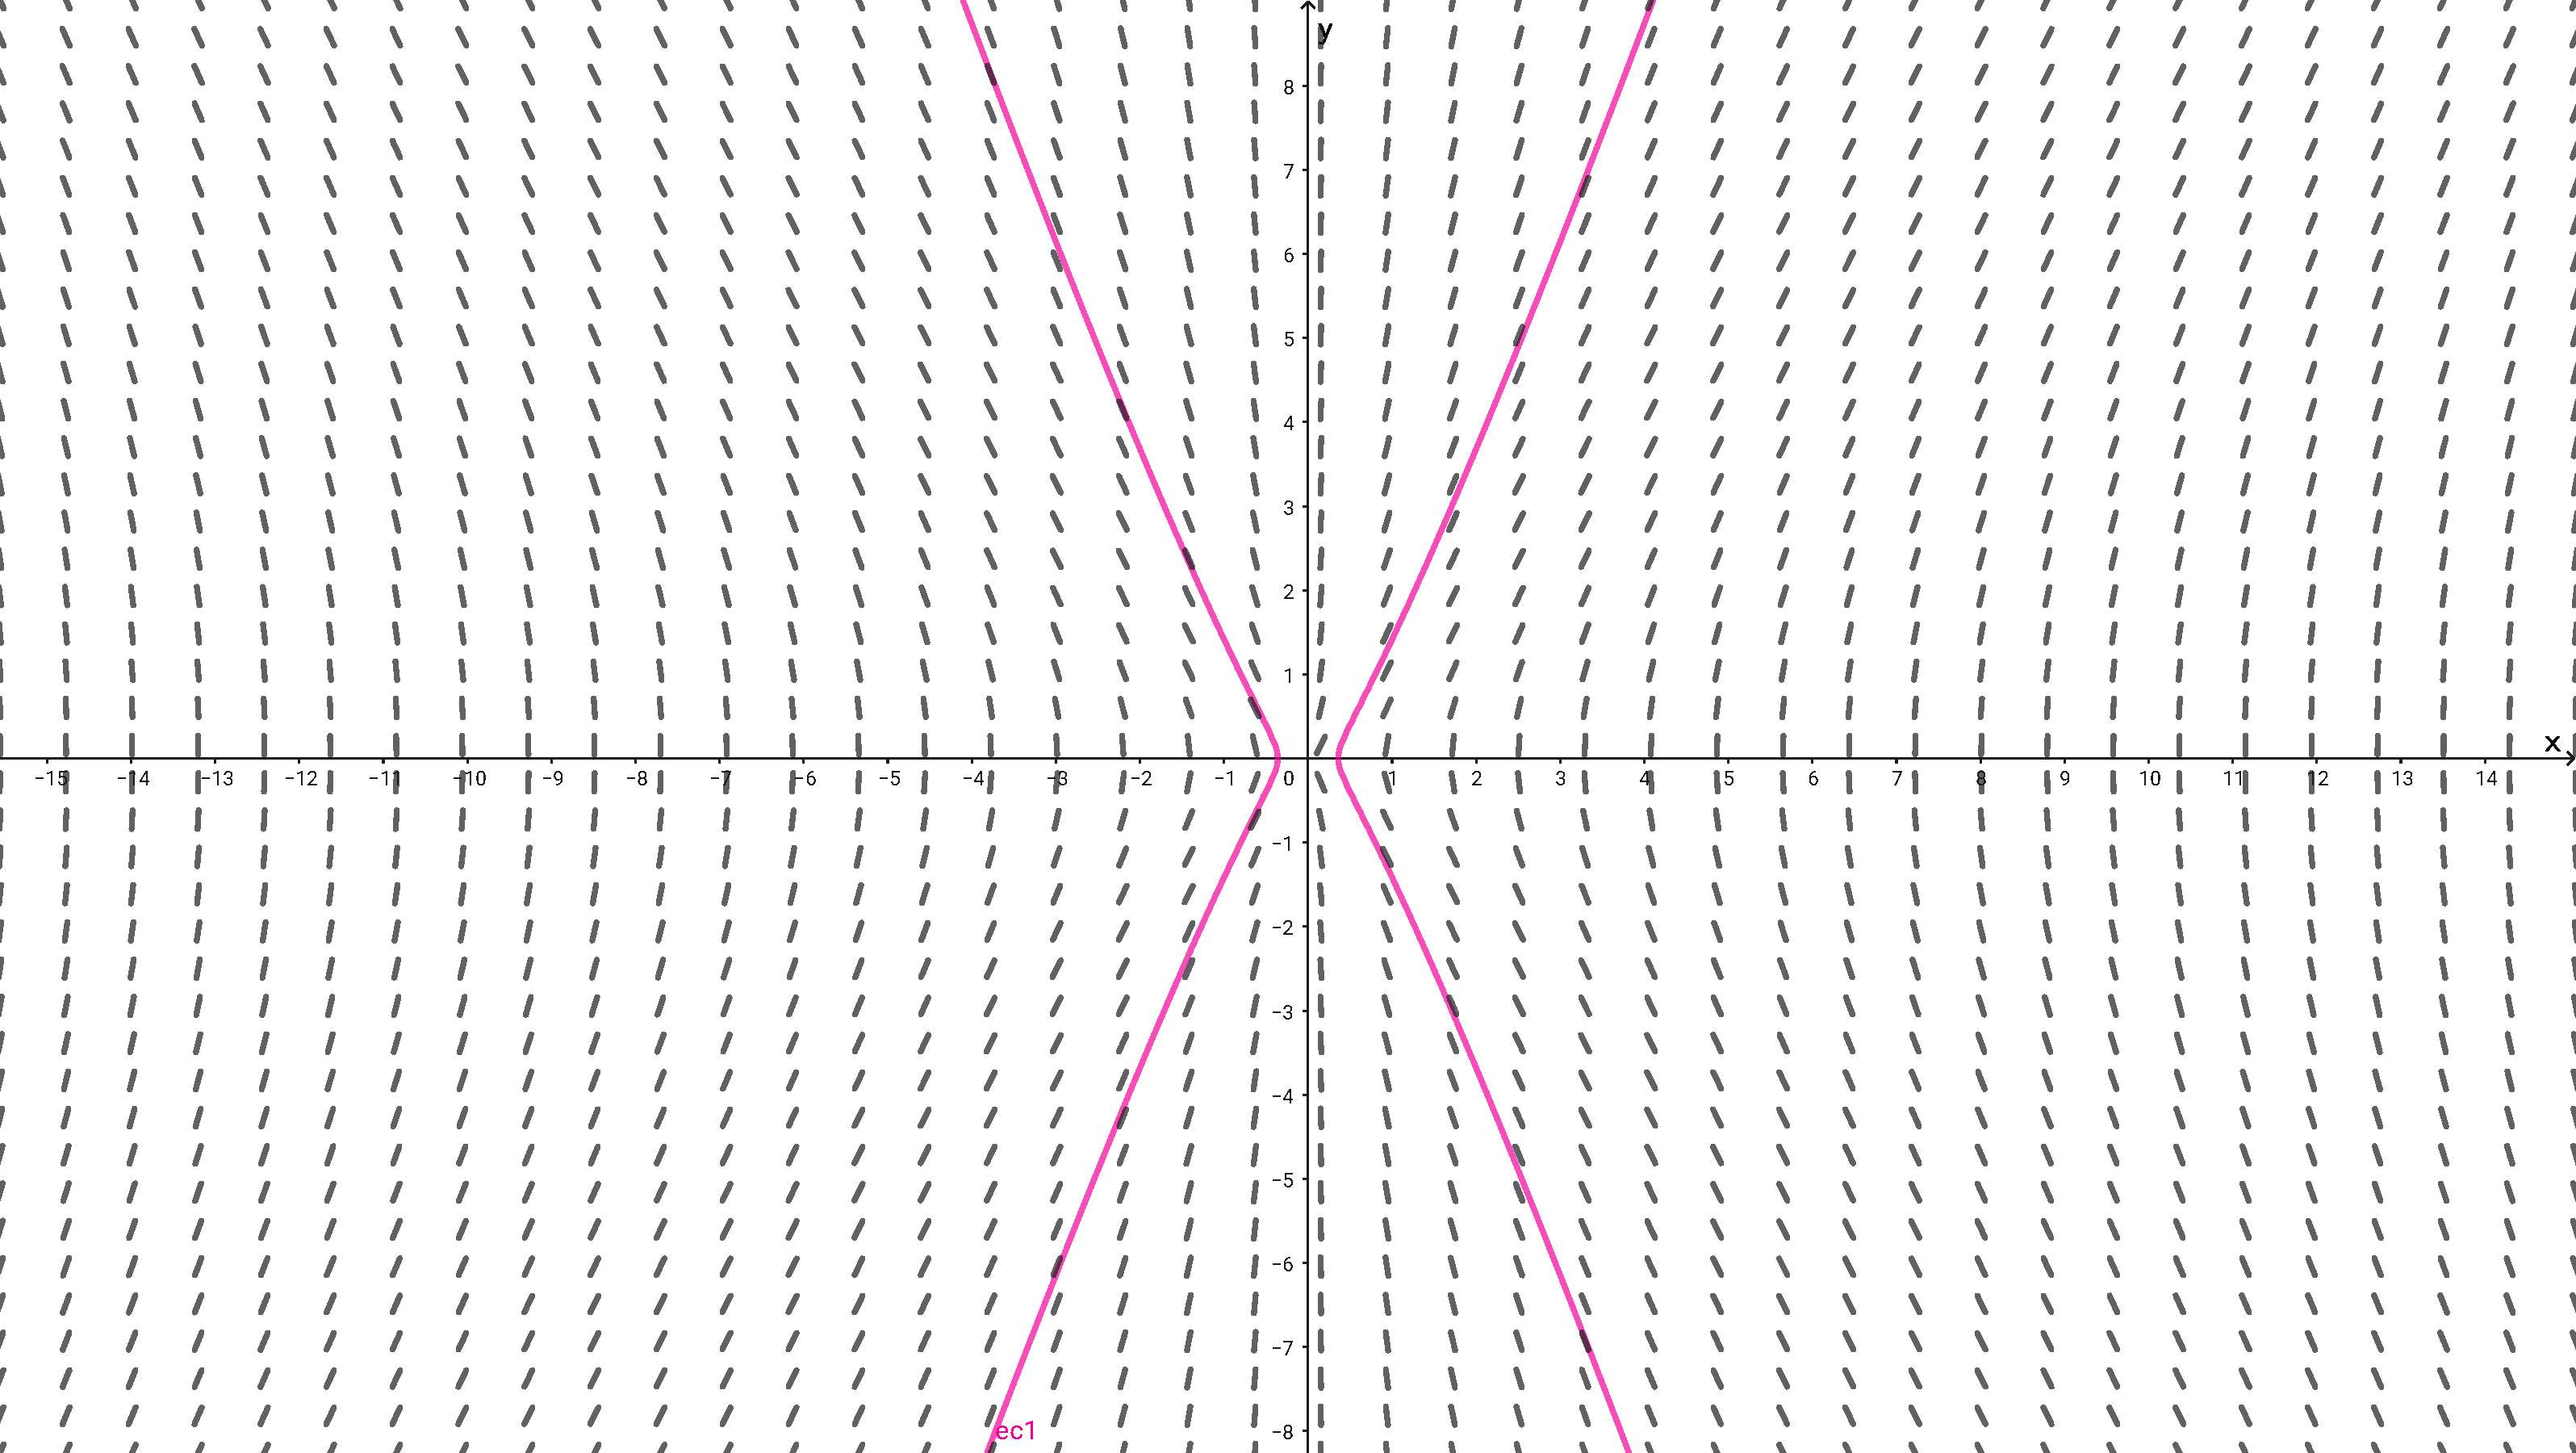
\includegraphics[width=0.72\textwidth]{img/unidad1_bloque3_ejercicio3.pdf}
    \caption{Bloque 3 — Ejercicio 3. Curvas implícitas $y^2 = 2x^2\ln|x| + Cx^2$ de la EDO homogénea $dy/dx = (x^2 + y^2)/(xy)$.}
\end{figure}

\textbf{Ejercicio 4.} $y' = \dfrac{x + 4y}{2x}$

\textit{Solución:}

Sustitución $y = ux$:
\begin{align*}
u + x\dfrac{du}{dx} &= \dfrac{1 + 4u}{2} \\[4pt]
x\dfrac{du}{dx} &= \dfrac{1 + 4u}{2} - u = \dfrac{1 + 2u}{2}
\end{align*}

Separando:
\[
\int \dfrac{2\,du}{1 + 2u} = \int \dfrac{dx}{x} \implies \ln|1 + 2u| = \ln|x| + c
\]
\[
1 + \dfrac{2y}{x} = Cx \implies x + 2y = Cx^2 \implies y = \dfrac{Cx^2 - x}{2}
\]

Verificación: $y' = \dfrac{2Cx - 1}{2}$.
\[
\dfrac{x + 4\cdot\tfrac{Cx^2 - x}{2}}{2x} = \dfrac{x + 2Cx^2 - 2x}{2x} = \dfrac{2Cx - 1}{2}
\]
\[
\boxed{\dfrac{2Cx - 1}{2} = \dfrac{2Cx - 1}{2} \quad \checkmark}
\]

\begin{figure}[H]
    \centering
    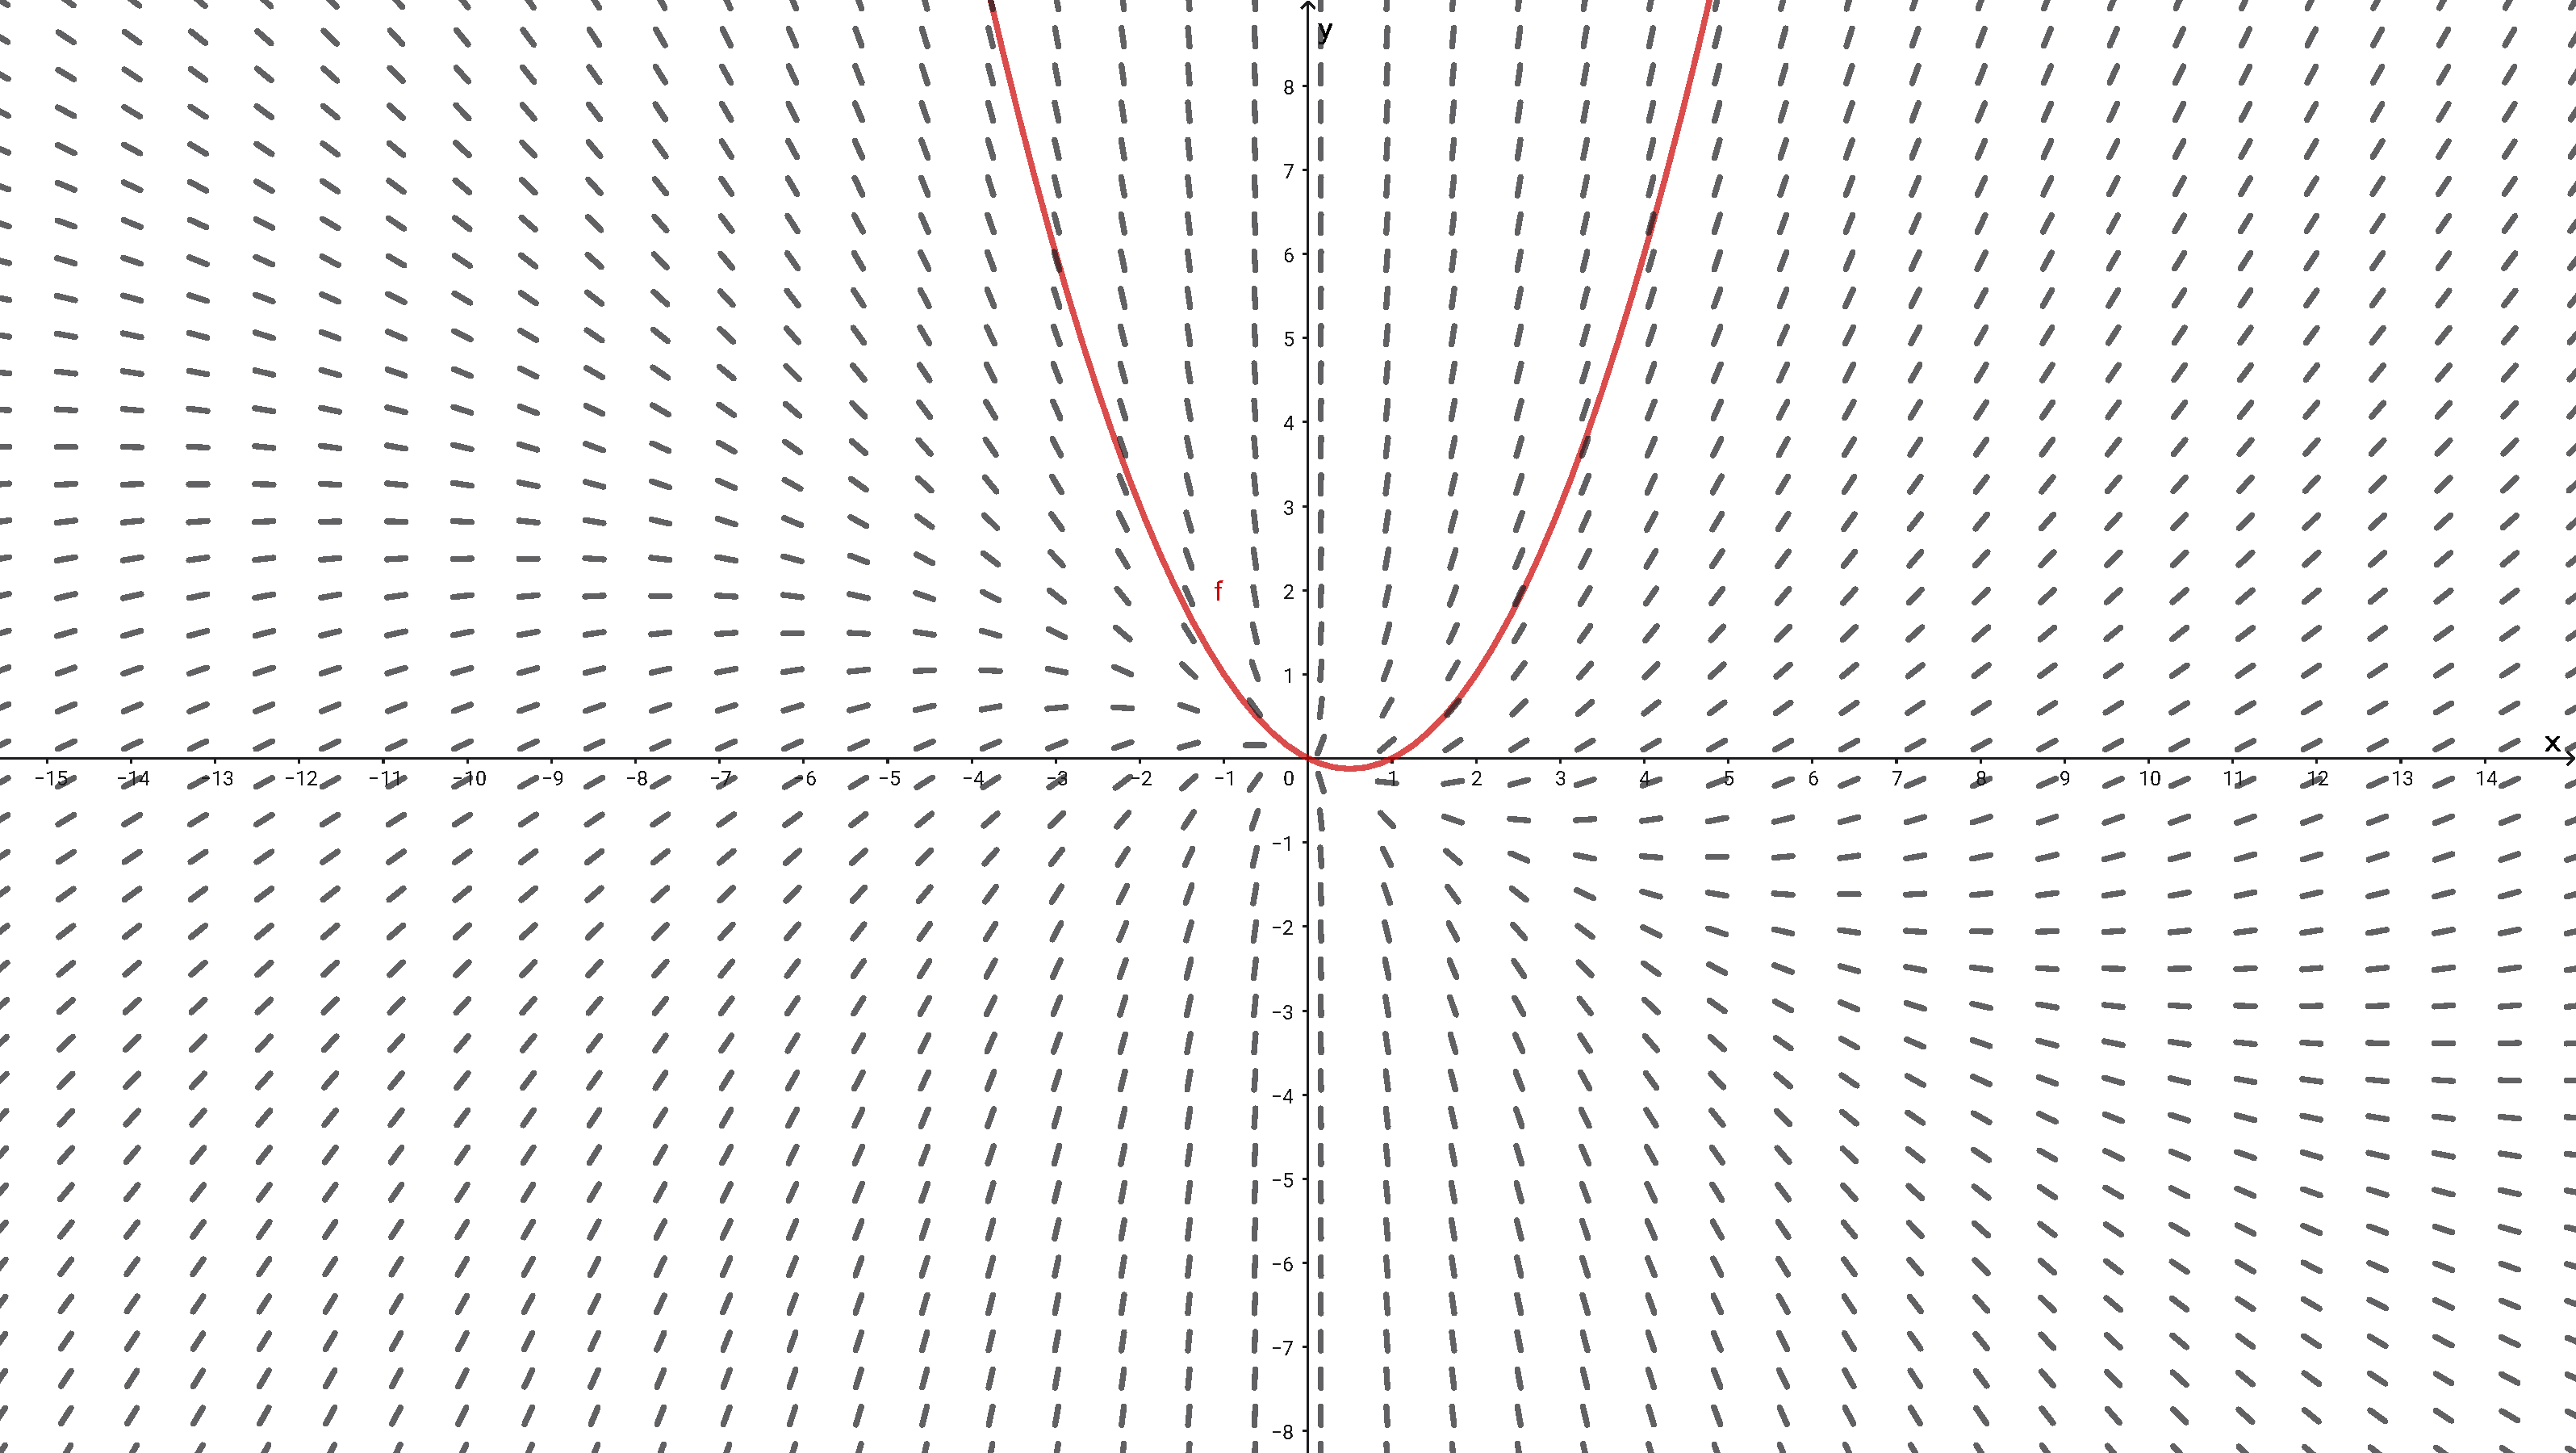
\includegraphics[width=0.72\textwidth]{img/unidad1_bloque3_ejercicio4.pdf}
    \caption{Bloque 3 — Ejercicio 4. Familia de parábolas $y = (Cx^2 - x)/2$ de la EDO homogénea $y' = (x + 4y)/(2x)$.}
\end{figure}

\textbf{Ejercicio 5.} $y' = \dfrac{2x + y^2}{xy}$

\textit{Solución:}

$M = -(2x + y^2)$, $N = xy$: $M$ es de grado 1 mientras $N$ es de grado 2, por lo que se verifica que la ecuación admite tratamiento con $y = ux$ tras reescribirla como $(2x + y^2)\,dx - xy\,dy = 0$. Sustitución $y = ux$, $dy = u\,dx + x\,du$:

\begin{align*}
(2x + u^2 x^2)\,dx - x\cdot ux(u\,dx + x\,du) &= 0 \\[4pt]
(2x + u^2 x^2 - u^2 x^2)\,dx - ux^3\,du &= 0 \\[4pt]
2x\,dx &= ux^3\,du \\[4pt]
2x^{-2}\,dx &= u\,du
\end{align*}

Integrando:
\[
2\int x^{-2}\,dx = \int u\,du \implies -\dfrac{2}{x} = \dfrac{u^2}{2}
\]

Revirtiendo $u = y/x$:
\[
-\dfrac{2}{x} = \dfrac{y^2}{2x^2} \implies \boxed{y^2 = -4x}
\]

\begin{figure}[H]
    \centering
    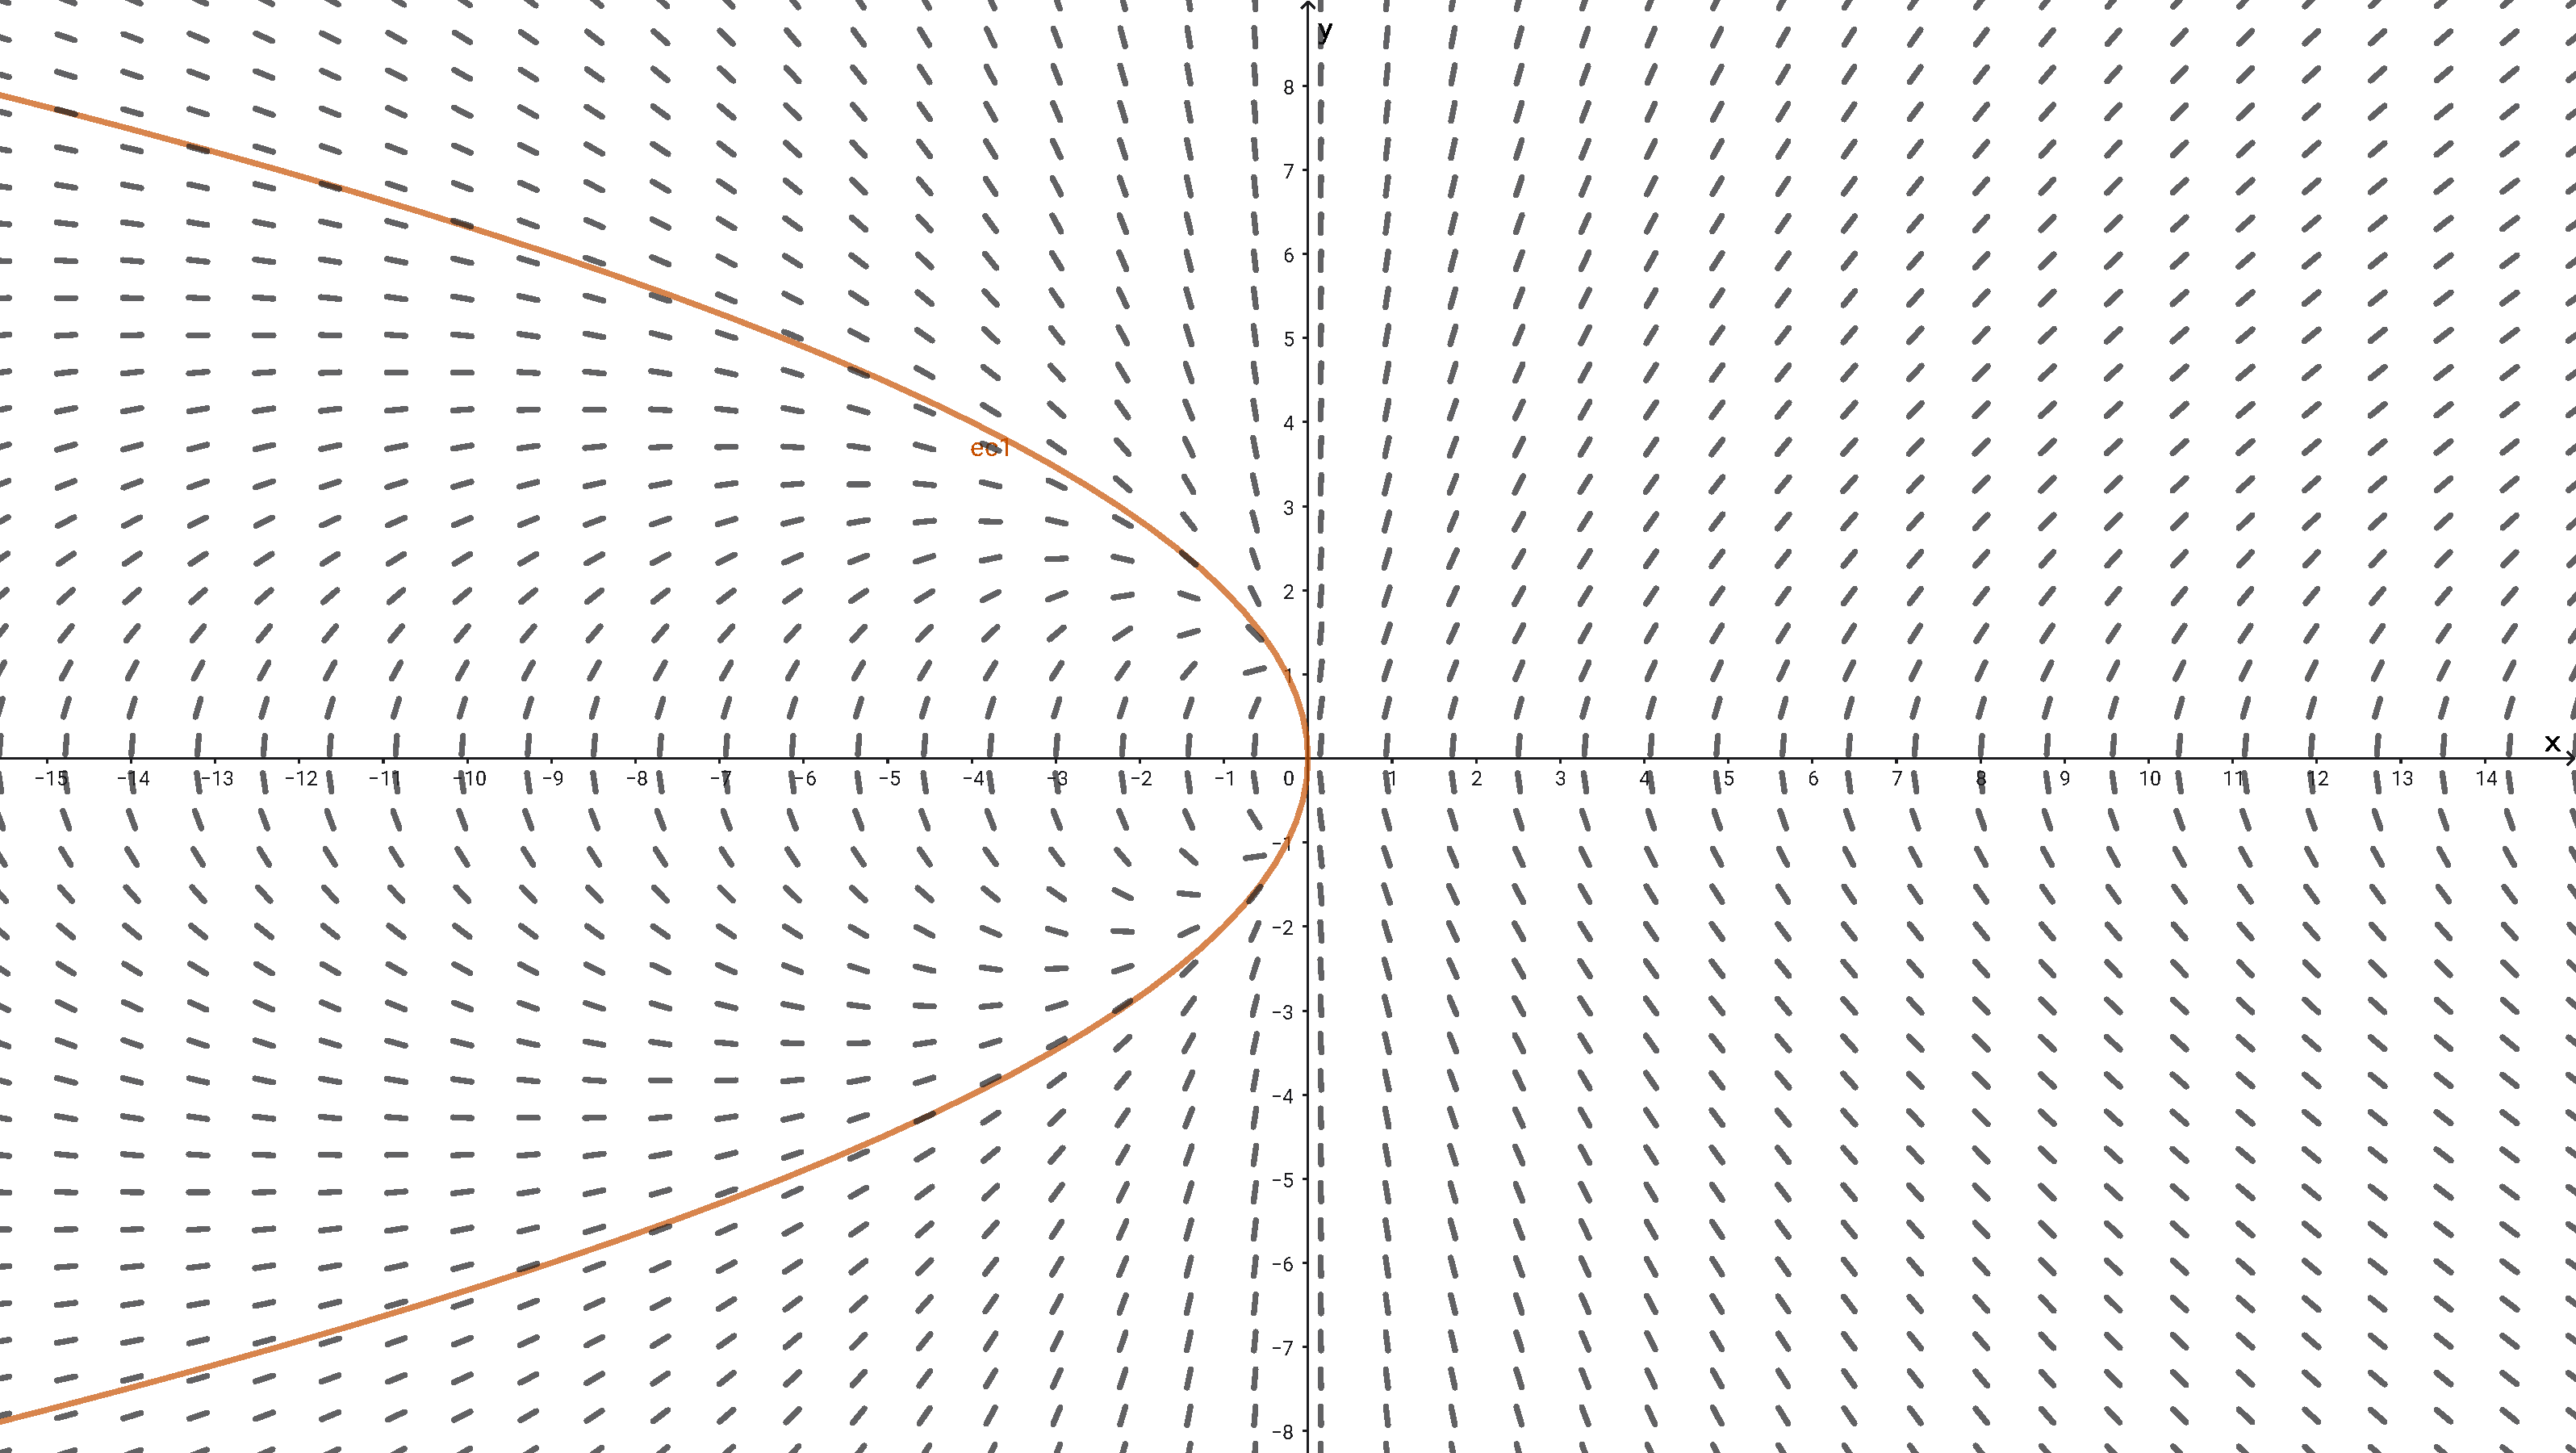
\includegraphics[width=0.72\textwidth]{img/unidad1_bloque3_ejercicio5.pdf}
    \caption{Bloque 3 — Ejercicio 5. Parábola horizontal $y^2 = -4x$ de la EDO homogénea $y' = (2x + y^2)/(xy)$.}
\end{figure}

% ============================================================

\section{Ecuaciones Diferenciales Lineales}

\subsection{Forma Estándar $y' + P(x)y = Q(x)$}

Una ecuación diferencial de primer orden es \textbf{lineal} cuando admite la forma estándar:
\begin{equation*}
y' + P(x)\,y = Q(x)
\end{equation*}

donde $P(x)$ y $Q(x)$ son funciones continuas de $x$ en un intervalo dado. La variable dependiente $y$ y su derivada $y'$ aparecen en forma lineal, sin potencias ni productos entre sí. Cuando $Q(x) = 0$ la ecuación se denomina \textbf{homogénea lineal}; en caso contrario es \textbf{no homogénea}.

El conjunto de soluciones de la ecuación no homogénea está formado por la suma de la solución general de la ecuación homogénea asociada más una solución particular de la completa.

\subsection{Método del Factor Integrante $\mu = e^{\int P(x)\,dx}$}

El método del \textbf{factor integrante} consiste en multiplicar ambos miembros por:
\[
\mu(x) = e^{\int P(x)\,dx}
\]

de manera que el miembro izquierdo se convierte exactamente en la derivada del producto $\mu(x)\,y$:
\[
\dfrac{d}{dx}\!\left[\mu(x)\,y\right] = \mu(x)\,Q(x)
\]

Integrando ambos miembros:
\[
\mu(x)\,y = \int \mu(x)\,Q(x)\,dx + C
\]

y, despejando,
\[
y = \dfrac{1}{\mu(x)}\left[\int \mu(x)\,Q(x)\,dx + C\right]
\]

\subsection{Ejercicios: Ecuaciones Lineales (Bloque 4, parte 2)}

Los ejercicios de este bloque corresponden a ecuaciones lineales de primer orden resueltas mediante el factor integrante. Los enunciados provienen de las ecuaciones de Bernoulli ya linealizadas: ver Sección~1.5.

% ============================================================

\section{Ecuaciones de Bernoulli}

\subsection{Estructura No Lineal y Parámetro $n$}

La \textbf{ecuación de Bernoulli} es una ecuación diferencial de primer orden no lineal de la forma:
\begin{equation*}
y' + P(x)\,y = Q(x)\,y^{n}
\end{equation*}

donde $n \in \mathbb{R}$ y $n \neq 0$, $n \neq 1$. Para $n = 0$ se reduce a una ecuación lineal directa; para $n = 1$ es una ecuación de variables separables. El parámetro $n$ controla el grado de no linealidad: la presencia del factor $y^n$ en el miembro derecho impide aplicar directamente el método del factor integrante.

Jacob Bernoulli planteó esta familia de ecuaciones en 1695. Leibniz propuso la sustitución que la transforma en lineal, solución que Bernoulli había buscado sin éxito. El resultado ilustra cómo una transformación algebraica adecuada puede reducir un problema no lineal a uno lineal, estrategia central en el análisis de sistemas dinámicos modernos.

\subsection{Transformación a Lineal mediante $u = y^{1-n}$}

La sustitución que linealiza la ecuación de Bernoulli es:
\[
u = y^{1-n}
\]

Diferenciando con respecto a $x$:
\[
\dfrac{du}{dx} = (1 - n)\,y^{-n}\,\dfrac{dy}{dx}
\]

Multiplicando la ecuación original por $(1 - n)\,y^{-n}$ y sustituyendo $u$ se obtiene la ecuación lineal:
\begin{equation*}
\dfrac{du}{dx} + (1 - n)\,P(x)\,u = (1 - n)\,Q(x)
\end{equation*}

que se resuelve con el factor integrante $\mu = e^{(1-n)\int P(x)\,dx}$. Finalizado el proceso, se revierte la sustitución mediante $y = u^{1/(1-n)}$.

\subsection{Ejercicios: Ecuaciones de Bernoulli (Bloque 4, parte 1)}

\textbf{Ejercicio 1.} $\dfrac{dy}{dx} - y = 2e^{x}y^{2}$ \quad ($n = 2$)

\textit{Solución:}

\textit{Paso 1.} Identificación: $P(x) = -1$, $Q(x) = 2e^{x}$, $n = 2$.

\textit{Paso 2.} Sustitución: $u = y^{1-2} = y^{-1}$, por tanto $y = u^{-1}$ y $\dfrac{dy}{dx} = -u^{-2}\dfrac{du}{dx}$.

\textit{Paso 3.} Multiplicar la ecuación original por $(-1)\,y^{-2} = (-1)u^{2}$:
\[
-u^{2}\!\left(-u^{-2}\dfrac{du}{dx} - u^{-1}\right) = -u^{2}\cdot 2e^{x}u^{-2}
\]
\[
\dfrac{du}{dx} + u = -2e^{x}
\]

\textit{Paso 4.} Ecuación lineal: $P^{*} = 1$, $Q^{*} = -2e^{x}$.

\textit{Paso 5.} Factor integrante: $\mu = e^{\int 1\,dx} = e^{x}$.

\textit{Paso 6.} Integración:
\begin{align*}
\dfrac{d}{dx}\!\left[u\,e^{x}\right] &= -2e^{x}\cdot e^{x} = -2e^{2x} \\[4pt]
u\,e^{x} &= \int -2e^{2x}\,dx = -e^{2x} + C \\[4pt]
u &= -e^{x} + Ce^{-x}
\end{align*}

\textit{Paso 7.} Reversión $u = y^{-1}$:
\[
\boxed{y = \dfrac{1}{Ce^{-x} - e^{x}}}
\]

\textbf{Ejercicio 2.} $y' + y = xy^{2}$ \quad ($n = 2$)

\textit{Solución:}

\textit{Paso 1.} $P(x) = 1$, $Q(x) = x$, $n = 2$.

\textit{Paso 2.} $u = y^{-1}$; $\dfrac{dy}{dx} = -u^{-2}\dfrac{du}{dx}$.

\textit{Paso 3.} Multiplicando por $-y^{-2}$:
\[
\dfrac{du}{dx} - u = -x
\]

\textit{Paso 4.} $P^{*} = -1$, $Q^{*} = -x$.

\textit{Paso 5.} $\mu = e^{-x}$.

\textit{Paso 6.} Integración por partes:
\begin{align*}
\dfrac{d}{dx}\!\left[u\,e^{-x}\right] &= -x\,e^{-x} \\[4pt]
u\,e^{-x} &= -\int x\,e^{-x}\,dx = x\,e^{-x} + e^{-x} + C \\[4pt]
u &= x + 1 + Ce^{x}
\end{align*}

\textit{Paso 7.} Reversión:
\[
\boxed{y = \dfrac{1}{x + 1 + Ce^{x}}}
\]

\textbf{Ejercicio 3.} $x\dfrac{dy}{dx} - y = \dfrac{x^{2}}{y^{2}}$ \quad ($n = -2$)

\textit{Solución:}

\textit{Paso 1.} Reescribir en forma estándar dividiendo entre $x$:
\[
\dfrac{dy}{dx} - \dfrac{1}{x}\,y = \dfrac{x}{y^{2}}
\]

$P(x) = -\dfrac{1}{x}$, $Q(x) = x$, $n = -2$.

\textit{Paso 2.} $u = y^{1-(-2)} = y^{3}$; entonces $y = u^{1/3}$ y $\dfrac{dy}{dx} = \dfrac{1}{3}u^{-2/3}\dfrac{du}{dx}$.

\textit{Paso 3.} Multiplicando la ecuación por $3y^{2} = 3u^{2/3}$:
\begin{align*}
3u^{2/3}\cdot\dfrac{1}{3}u^{-2/3}\dfrac{du}{dx} - 3u^{2/3}\cdot\dfrac{u^{1/3}}{x} &= 3u^{2/3}\cdot xu^{-2/3} \\[4pt]
\dfrac{du}{dx} - \dfrac{3}{x}\,u &= 3x
\end{align*}

\textit{Paso 4.} Ecuación lineal resultante: $\dfrac{du}{dx} - \dfrac{3}{x}\,u = 3x$.

\textit{Paso 5.} Factor integrante: $\mu = e^{\int -3/x\,dx} = e^{-3\ln|x|} = x^{-3}$.

\textit{Paso 6.} Integración:
\begin{align*}
\dfrac{d}{dx}\!\left[u\,x^{-3}\right] &= 3x\cdot x^{-3} = 3x^{-2} \\[4pt]
u\,x^{-3} &= \int 3x^{-2}\,dx = -3x^{-1} + C \\[4pt]
u &= -3x^{2}\cdot x^{-1}\cdot x^{3-3}\cdot x + Cx^{3} = -3x^{2} + Cx^{3}
\end{align*}

\textit{Paso 7.} Reversión $u = y^{3}$:
\[
\boxed{y^{3} = Cx^{3} - 3x^{2} \implies y = \left(Cx^{3} - 3x^{2}\right)^{1/3}}
\]

% ============================================================

\section{Aplicaciones en Ingeniería de Software}

Las ecuaciones diferenciales de primer orden no son exclusivas del análisis de circuitos o de la mecánica clásica. En el contexto de la ingeniería de software, emergen naturalmente al modelar la evolución temporal de métricas de sistema: volúmenes de datos, tasas de procesamiento, densidad de conexiones en una red y propagación de información. Las dos subsecciones siguientes presentan modelos concretos y representativos.

\subsection{Modelado de Tasas de Crecimiento en Bases de Datos}

El volumen de registros almacenados en una base de datos operativa crece en función tanto de la actividad de escritura de los usuarios como de procesos automáticos de generación de datos. Bajo la hipótesis de que la tasa de inserción neta es proporcional al volumen actual más una tasa de ingreso exógena constante, el modelo diferencial es:

\begin{equation*}
\dfrac{dV}{dt} = kV + \lambda
\end{equation*}

donde $V(t)$ es el volumen de registros en el instante $t$, $k > 0$ es la constante de crecimiento orgánico y $\lambda \geq 0$ es la tasa de ingreso externa. Esta ecuación es lineal de primer orden con la forma estándar:
\[
\dfrac{dV}{dt} - kV = \lambda
\]

Factor integrante: $\mu = e^{-kt}$.

\begin{align*}
\dfrac{d}{dt}\!\left[V\,e^{-kt}\right] &= \lambda\,e^{-kt} \\[4pt]
V\,e^{-kt} &= \int \lambda\,e^{-kt}\,dt = -\dfrac{\lambda}{k}\,e^{-kt} + C \\[4pt]
V(t) &= Ce^{kt} - \dfrac{\lambda}{k}
\end{align*}

Aplicando la condición inicial $V(0) = V_0$:
\[
V_0 = C - \dfrac{\lambda}{k} \implies C = V_0 + \dfrac{\lambda}{k}
\]
\[
\boxed{V(t) = \left(V_0 + \dfrac{\lambda}{k}\right)e^{kt} - \dfrac{\lambda}{k}}
\]

Este modelo es aplicable en la planificación de capacidad de almacenamiento: dado $V_0$, $k$ y $\lambda$ estimados a partir de métricas históricas, el ingeniero puede calcular cuándo el volumen superará un umbral crítico $V_{\max}$, resolviendo:
\[
t^* = \dfrac{1}{k}\ln\!\left(\dfrac{V_{\max} + \lambda/k}{V_0 + \lambda/k}\right)
\]

y dimensionar la infraestructura con la antelación necesaria.

\subsection{Dinámica de Propagación de Información en Redes}

El modelo SI (\textit{Susceptible–Infected}) describe la difusión de un mensaje, una vulnerabilidad o un protocolo actualizado en una red de $N$ nodos. Sea $I(t)$ el número de nodos que han adoptado la información al tiempo $t$. Si la tasa de propagación es proporcional al producto entre los nodos ya informados y los aún no informados, la ecuación resultante es:
\begin{equation*}
\dfrac{dI}{dt} = \beta\, I\!\left(N - I\right)
\end{equation*}

donde $\beta > 0$ es la tasa de contacto efectivo. Esta ecuación es separable:
\[
\dfrac{dI}{I(N - I)} = \beta\,dt
\]

Descomposición en fracciones parciales:
\[
\dfrac{1}{I(N - I)} = \dfrac{1}{N}\!\left(\dfrac{1}{I} + \dfrac{1}{N - I}\right)
\]

Integrando:
\begin{align*}
\dfrac{1}{N}\!\left(\ln|I| - \ln|N - I|\right) &= \beta\,t + c \\[4pt]
\ln\!\left(\dfrac{I}{N - I}\right) &= N\beta\,t + C_0 \\[4pt]
\dfrac{I}{N - I} &= A\,e^{N\beta t}
\end{align*}

Despejando $I(t)$ y aplicando la condición inicial $I(0) = I_0$:
\[
A = \dfrac{I_0}{N - I_0}
\]
\[
\boxed{I(t) = \dfrac{N\,I_0\,e^{N\beta t}}{N - I_0 + I_0\,e^{N\beta t}}}
\]

La solución corresponde a la curva logística: crecimiento inicialmente exponencial que se desacelera al saturarse la red. En ingeniería de software, este modelo es útil para estimar el tiempo de convergencia de actualizaciones en sistemas distribuidos, evaluar la velocidad de propagación de parches de seguridad o analizar la dinámica de adopción de una nueva API en una red de microservicios.

\section{Aplicaciones Multidisciplinarias de las Ecuaciones Diferenciales}

Las ecuaciones diferenciales de primer orden no constituyen un objeto puramente abstracto: son el lenguaje matemático con el que la ciencia y la ingeniería describen el cambio. Su presencia atraviesa disciplinas que van desde la física clásica hasta la biología computacional y la economía cuantitativa.

\subsection{Física e Ingeniería Eléctrica}

En circuitos eléctricos de corriente continua, la carga $q(t)$ en un condensador conectado en serie con una resistencia $R$ y una fuente de tensión $V_0$ satisface la ecuación lineal de primer orden:
\[
 R\,\dfrac{dq}{dt} + \dfrac{q}{C} = V_0
\]
La solución, obtenida mediante el factor integrante $\mu = e^{t/(RC)}$, es:
\[
 q(t) = CV_0\!\left(1 - e^{-t/(RC)}\right) + q_0\,e^{-t/(RC)}
\]
donde $\tau = RC$ es la constante de tiempo del circuito. Este resultado es fundamental en el diseño de filtros, temporizadores y convertidores analógico-digitales.

\subsection{Mecánica: Caída con Resistencia de Aire}

Para un cuerpo de masa $m$ que cae bajo la acción de la gravedad $g$ con resistencia aerodinámica proporcional a la velocidad $v(t)$, la segunda ley de Newton produce:
\[
m\,\dfrac{dv}{dt} = mg - kv
\]
Esta es una ecuación lineal de primer orden con solución:
\[
v(t) = \dfrac{mg}{k}\!\left(1 - e^{-kt/m}\right)
\]
La velocidad terminal $v_{\infty} = mg/k$ se alcanza asintóticamente, resultado de equilibrar la fuerza gravitacional con la resistencia del medio.

\subsection{Biología: Dinámica Poblacional}

El modelo de crecimiento logístico de Verhulst describe la evolución de una población $P(t)$ bajo capacidad de carga $K$:
\[
\dfrac{dP}{dt} = rP\!\left(1 - \dfrac{P}{K}\right)
\]
Esta ecuación de Bernoulli con $n = 2$ se linealiza con $u = P^{-1}$ y su solución es la curva sigmoidea:
\[
P(t) = \dfrac{KP_0}{P_0 + (K - P_0)e^{-rt}}
\]
Es el modelo base en epidemiología computacional, ecología y análisis de tasas de adopción de tecnología.

\subsection{Química: Cinética de Reacción de Primer Orden}

La concentración $C(t)$ de un reactivo que se consume a una tasa proporcional a su concentración satisface:
\[
\dfrac{dC}{dt} = -kC \implies C(t) = C_0\,e^{-kt}
\]
El modelo tiene aplicación directa en el cálculo de vida media de fármacos, desintegración radiactiva y análisis de estabilidad de compuestos en sistemas de almacenamiento de datos bioquímicos.

\subsection{Economía: Depreciación y Acumulación de Capital}

En macroeconomía, el stock de capital $K(t)$ en un modelo simplificado evoluciona según:
\[
\dfrac{dK}{dt} = sY - \delta K
\]
donde $s$ es la tasa de ahorro, $Y$ el producto e.g. constante, y $\delta$ la tasa de depreciación. Esta ecuación lineal tiene la solución de estado estacionario $K^* = sY/\delta$, que el capital alcanza exponencialmente. El mismo modelo se aplica al análisis de depreciación de activos tecnológicos en empresas de software.

\subsection{Inteligencia Artificial: Descenso de Gradiente Continuo}

El algoritmo de descenso de gradiente en su formulación continua actualiza los parámetros $\theta(t)$ de un modelo según:
\[
\dfrac{d\theta}{dt} = -\eta\,\nabla_{\theta}\mathcal{L}(\theta)
\]
donde $\eta > 0$ es la tasa de aprendizaje y $\mathcal{L}$ es la función de pérdida. Para problemas cuadráticos con $\mathcal{L} = \frac{1}{2}A\theta^2 - b\theta$, esto produce una EDO lineal cuya solución converge exponencialmente al mínimo. El análisis del espectro de autovalores de la Hessiana de $\mathcal{L}$ determina la tasa de convergencia, conectando la teoría de EDO con la optimización en aprendizaje profundo.

\subsection{Síntesis}

Las ecuaciones diferenciales de primer orden son ubicuas: cada disciplina reduce sus leyes fundamentales de cambio a una de las formas estudiadas en esta unidad. La clasificación sistemática (separables, homogéneas, lineales, Bernoulli) no es un ejercicio taxonómico sino una guía operativa que permite al ingeniero identificar el método de solución adecuado en función de la estructura algebraica del modelo.

% ==================== UNIDAD II ====================
\chapter{Unidad II: Transformada de Laplace}

La Transformada de Laplace es una herramienta de análisis funcional que convierte una ecuación diferencial ordinaria definida en el dominio del tiempo en una ecuación algebraica en el dominio de la variable compleja $s$. Esta conversión reduce el problema de resolver una EDO, con sus condiciones iniciales, a la resolución de una ecuación algebraica seguida de una transformación inversa. Su eficacia es especialmente notable en el análisis de sistemas lineales e invariantes en el tiempo, campo de aplicación directa en ingeniería de software para el modelado de sistemas de control, colas de procesamiento y redes de comunicación.

La Transformada de Laplace de una función $f(t)$ definida para $t \geq 0$ se define formalmente como la integral impropia:
\begin{equation*}
\mathcal{L}\{f(t)\} = F(s) = \int_{0}^{\infty} e^{-st}\,f(t)\,dt
\end{equation*}

donde $s \in \mathbb{C}$ con $\Re(s)$ suficientemente grande para garantizar la convergencia de la integral. La notación $F(s) = \mathcal{L}\{f(t)\}$ pone de manifiesto la correspondencia biyectiva entre el espacio de funciones del tiempo y el espacio de transformadas, asumidas las condiciones de continuidad a trozos y orden exponencial que aseguran la existencia de la integral.

\section{Transformada de Laplace Directa}

\subsection{Definición Integral y Convergencia}

El operador $\mathcal{L}$ es lineal: para constantes $\alpha, \beta$ y funciones $f(t)$, $g(t)$ con transformadas existentes,
\begin{equation*}
\mathcal{L}\{\alpha f(t) + \beta g(t)\} = \alpha\,\mathcal{L}\{f(t)\} + \beta\,\mathcal{L}\{g(t)\}
\end{equation*}

La convergencia de la integral impropia requiere que $f(t)$ sea de orden exponencial; es decir, que existan constantes $M > 0$, $c \geq 0$ y $T \geq 0$ tales que $|f(t)| \leq Me^{ct}$ para todo $t > T$. Bajo esta condición, la integral converge absolutamente para $\Re(s) > c$.

\subsection{Ejercicios: Transformada Directa desde la Definición}

\textbf{Ejercicio 1.} $\mathcal{L}\{k\}$, $k$ constante.

\textit{Solución:}

Por definición:
\[
\mathcal{L}\{k\} = \int_{0}^{\infty} e^{-st}\cdot k\,dt = k\int_{0}^{\infty} e^{-st}\,dt
\]

Evaluando la integral impropia mediante el límite $b \to \infty$:
\begin{align*}
k\int_{0}^{\infty} e^{-st}\,dt &= k\lim_{b\to\infty}\left[-\dfrac{1}{s}e^{-st}\right]_{0}^{b} \\[4pt]
&= k\lim_{b\to\infty}\left(-\dfrac{e^{-sb}}{s} + \dfrac{1}{s}\right) \\[4pt]
&= k\left(0 + \dfrac{1}{s}\right) \qquad (\Re(s) > 0)
\end{align*}
\[
\boxed{\mathcal{L}\{k\} = \dfrac{k}{s}}
\]

\textbf{Ejercicio 2.} $\mathcal{L}\{t\}$

\textit{Solución:}

\[
\mathcal{L}\{t\} = \int_{0}^{\infty} e^{-st}\,t\,dt
\]

Integración por partes con $u = t$, $dv = e^{-st}\,dt$; entonces $du = dt$, $v = -\dfrac{1}{s}e^{-st}$:

\begin{align*}
\int_{0}^{\infty} t\,e^{-st}\,dt &= \left[-\dfrac{t}{s}e^{-st}\right]_{0}^{\infty} + \dfrac{1}{s}\int_{0}^{\infty} e^{-st}\,dt \\[4pt]
&= 0 + \dfrac{1}{s}\left[-\dfrac{1}{s}e^{-st}\right]_{0}^{\infty} \\[4pt]
&= \dfrac{1}{s}\cdot\dfrac{1}{s}
\end{align*}

El término de borde $\left[-\dfrac{t}{s}e^{-st}\right]_{0}^{\infty}$ se anula porque $\lim_{t\to\infty} t\,e^{-st} = 0$ para $\Re(s) > 0$ (la exponencial decrece más rápido que cualquier potencia).
\[
\boxed{\mathcal{L}\{t\} = \dfrac{1}{s^2}}
\]

\textbf{Ejercicio 3.} $\mathcal{L}\{t^2\}$

\textit{Solución:}

\[
\mathcal{L}\{t^2\} = \int_{0}^{\infty} e^{-st}\,t^2\,dt
\]

Primera integración por partes con $u = t^2$, $dv = e^{-st}\,dt$:
\begin{align*}
\int_{0}^{\infty} t^2\,e^{-st}\,dt &= \left[-\dfrac{t^2}{s}e^{-st}\right]_{0}^{\infty} + \dfrac{2}{s}\int_{0}^{\infty} t\,e^{-st}\,dt
\end{align*}

El término de borde se anula bajo la hipótesis de convergencia. Reutilizando el resultado del ejercicio anterior:
\begin{align*}
&= 0 + \dfrac{2}{s}\cdot\dfrac{1}{s^2} = \dfrac{2}{s^3}
\end{align*}
\[
\boxed{\mathcal{L}\{t^2\} = \dfrac{2}{s^3}}
\]

\textbf{Ejercicio 4.} $\mathcal{L}\{e^{-9t}\}$

\textit{Solución:}

\begin{align*}
\mathcal{L}\{e^{-9t}\} &= \int_{0}^{\infty} e^{-st}\,e^{-9t}\,dt = \int_{0}^{\infty} e^{-(s+9)t}\,dt \\[4pt]
&= \lim_{b\to\infty}\left[-\dfrac{1}{s+9}e^{-(s+9)t}\right]_{0}^{b} = \dfrac{1}{s+9} \qquad (\Re(s) > -9)
\end{align*}
\[
\boxed{\mathcal{L}\{e^{-9t}\} = \dfrac{1}{s+9}}
\]

\textbf{Ejercicio 5.} $\mathcal{L}\{\sin(\omega t)\}$

\textit{Solución:}

\[
\mathcal{L}\{\sin(\omega t)\} = \int_{0}^{\infty} e^{-st}\sin(\omega t)\,dt
\]

Se aplica la fórmula estándar de integración:
\[
\int e^{au}\sin(nu)\,du = \dfrac{e^{au}}{a^2 + n^2}\bigl(a\sin(nu) - n\cos(nu)\bigr) + C
\]

con $a = -s$ y $n = \omega$. Evaluando de $0$ a $\infty$ con $\Re(s) > 0$:

\begin{align*}
\left[\dfrac{e^{-st}}{s^2 + \omega^2}\bigl(-s\sin(\omega t) - \omega\cos(\omega t)\bigr)\right]_{0}^{\infty} &= 0 - \dfrac{1}{s^2 + \omega^2}(0 - \omega) \\[4pt]
&= \dfrac{\omega}{s^2 + \omega^2}
\end{align*}
\[
\boxed{\mathcal{L}\{\sin(\omega t)\} = \dfrac{\omega}{s^2 + \omega^2}}
\]

\textbf{Ejercicio 6.} $\mathcal{L}\{\cos^2(t)\}$

\textit{Solución:}

Se aplica la identidad trigonométrica $\cos^2(t) = \dfrac{1 + \cos(2t)}{2}$ y la linealidad del operador:

\begin{align*}
\mathcal{L}\{\cos^2(t)\} &= \dfrac{1}{2}\mathcal{L}\{1\} + \dfrac{1}{2}\mathcal{L}\{\cos(2t)\} \\[4pt]
&= \dfrac{1}{2}\cdot\dfrac{1}{s} + \dfrac{1}{2}\cdot\dfrac{s}{s^2 + 4}
\end{align*}
\[
\boxed{\mathcal{L}\{\cos^2(t)\} = \dfrac{1}{2s} + \dfrac{s}{2(s^2 + 4)}}
\]

% ============================================================

\section{Transformada de Laplace por Fórmulas y Propiedades}

\subsection{Formulario Fundamental y Propiedades Operacionales}

Las transformadas de las funciones elementales forman el formulario base. Las más utilizadas, que se deducen directamente de la definición integral, son:

\begin{align*}
\mathcal{L}\{1\} &= \dfrac{1}{s} &
\mathcal{L}\{t^n\} &= \dfrac{n!}{s^{n+1}} \\[6pt]
\mathcal{L}\{e^{at}\} &= \dfrac{1}{s - a} &
\mathcal{L}\{\sin(\omega t)\} &= \dfrac{\omega}{s^2 + \omega^2} \\[6pt]
\mathcal{L}\{\cos(\omega t)\} &= \dfrac{s}{s^2 + \omega^2} &
\mathcal{L}\{\sinh(at)\} &= \dfrac{a}{s^2 - a^2} \\[6pt]
\mathcal{L}\{\cosh(at)\} &= \dfrac{s}{s^2 - a^2} & &
\end{align*}

Las propiedades operacionales más empleadas son:

\begin{itemize}
    \item \textbf{Primer teorema de traslación (desplazamiento en $s$):} $\mathcal{L}\{e^{at}f(t)\} = F(s - a)$, donde $F(s) = \mathcal{L}\{f(t)\}$.
    \item \textbf{Derivada de la transformada:} $\mathcal{L}\{t^n f(t)\} = (-1)^n\dfrac{d^n}{ds^n}F(s)$.
    \item \textbf{Linealidad:} $\mathcal{L}\{\alpha f + \beta g\} = \alpha F(s) + \beta G(s)$.
\end{itemize}

\subsection{Ejercicios: Transformada por Fórmulas}

\textbf{Ejercicio 1.} $\mathcal{L}\{\sin(3t)\}$

\textit{Solución:}

Directamente del formulario con $\omega = 3$:
\[
\boxed{\mathcal{L}\{\sin(3t)\} = \dfrac{3}{s^2 + 9}}
\]

\textbf{Ejercicio 2.} $\mathcal{L}\{\cos^2(t)\}$

\textit{Solución:}

Identidad $\cos^2(t) = \dfrac{1 + \cos(2t)}{2}$ y linealidad:
\[
\mathcal{L}\{\cos^2(t)\} = \dfrac{1}{2}\cdot\dfrac{1}{s} + \dfrac{1}{2}\cdot\dfrac{s}{s^2 + 4}
\]
\[
\boxed{\mathcal{L}\{\cos^2(t)\} = \dfrac{1}{2s} + \dfrac{s}{2(s^2 + 4)}}
\]

\textbf{Ejercicio 3.} $\mathcal{L}\{e^{4t}\}$

\textit{Solución:}

Fórmula $\mathcal{L}\{e^{at}\} = \dfrac{1}{s-a}$ con $a = 4$:
\[
\boxed{\mathcal{L}\{e^{4t}\} = \dfrac{1}{s - 4}} \qquad (s > 4)
\]

\textbf{Ejercicio 4.} $\mathcal{L}\{(1 + e^{2t})^2\}$

\textit{Solución:}

Desarrollo algebraico del cuadrado y linealidad:
\begin{align*}
(1 + e^{2t})^2 &= 1 + 2e^{2t} + e^{4t}
\end{align*}
\begin{align*}
\mathcal{L}\{(1 + e^{2t})^2\} &= \mathcal{L}\{1\} + 2\mathcal{L}\{e^{2t}\} + \mathcal{L}\{e^{4t}\} \\[4pt]
&= \dfrac{1}{s} + \dfrac{2}{s - 2} + \dfrac{1}{s - 4}
\end{align*}
\[
\boxed{\mathcal{L}\{(1 + e^{2t})^2\} = \dfrac{1}{s} + \dfrac{2}{s - 2} + \dfrac{1}{s - 4}}
\]

\textbf{Ejercicio 5.} $\mathcal{L}\{4t\cos(5t)\}$

\textit{Solución:}

Se aplica la propiedad de derivada de la transformada con $n = 1$, $f(t) = \cos(5t)$, $F(s) = \dfrac{s}{s^2 + 25}$:
\[
\mathcal{L}\{t\cos(5t)\} = -\dfrac{d}{ds}\!\left[\dfrac{s}{s^2 + 25}\right]
\]

Regla del cociente:
\begin{align*}
\dfrac{d}{ds}\!\left[\dfrac{s}{s^2 + 25}\right] &= \dfrac{(s^2 + 25) - s\cdot 2s}{(s^2 + 25)^2} = \dfrac{25 - s^2}{(s^2 + 25)^2}
\end{align*}

Entonces $\mathcal{L}\{t\cos(5t)\} = \dfrac{s^2 - 25}{(s^2 + 25)^2}$. Por linealidad:
\[
\boxed{\mathcal{L}\{4t\cos(5t)\} = \dfrac{4(s^2 - 25)}{(s^2 + 25)^2}}
\]

\textbf{Ejercicio 6.} $\mathcal{L}\{t^2\cos(t)\}$

\textit{Solución:}

Propiedad de derivada con $n = 2$, $f(t) = \cos(t)$, $F(s) = \dfrac{s}{s^2 + 1}$:
\[
\mathcal{L}\{t^2\cos(t)\} = (-1)^2\dfrac{d^2}{ds^2}\!\left[\dfrac{s}{s^2 + 1}\right] = \dfrac{d^2}{ds^2}\!\left[\dfrac{s}{s^2 + 1}\right]
\]

Primera derivada:
\[
\dfrac{d}{ds}\!\left[\dfrac{s}{s^2 + 1}\right] = \dfrac{1 - s^2}{(s^2 + 1)^2}
\]

Segunda derivada (regla del cociente):
\begin{align*}
\dfrac{d}{ds}\!\left[\dfrac{1 - s^2}{(s^2 + 1)^2}\right] &= \dfrac{-2s(s^2 + 1)^2 - (1 - s^2)\cdot 2(s^2 + 1)\cdot 2s}{(s^2 + 1)^4} \\[4pt]
&= \dfrac{-2s(s^2 + 1) - 4s(1 - s^2)}{(s^2 + 1)^3} \\[4pt]
&= \dfrac{-2s^3 - 2s - 4s + 4s^3}{(s^2 + 1)^3} \\[4pt]
&= \dfrac{2s^3 - 6s}{(s^2 + 1)^3}
\end{align*}
\[
\boxed{\mathcal{L}\{t^2\cos(t)\} = \dfrac{2s^3 - 6s}{(s^2 + 1)^3}}
\]

\textbf{Ejercicio 7.} $\mathcal{L}\{t^2 e^{t}\cos(t)\}$

\textit{Solución:}

Se combina el resultado anterior con el primer teorema de traslación. Sea $F(s) = \mathcal{L}\{t^2\cos(t)\} = \dfrac{2s^3 - 6s}{(s^2 + 1)^3}$.

Por traslación con $a = 1$, sustituir $s \to s - 1$:
\begin{align*}
\mathcal{L}\{e^{t}\cdot t^2\cos(t)\} &= F(s - 1) = \dfrac{2(s-1)^3 - 6(s-1)}{\bigl((s-1)^2 + 1\bigr)^3}
\end{align*}

Desarrollo del numerador:
\begin{align*}
2(s-1)^3 - 6(s-1) &= 2(s^3 - 3s^2 + 3s - 1) - 6s + 6 \\[4pt]
&= 2s^3 - 6s^2 + 6s - 2 - 6s + 6 = 2s^3 - 6s^2 + 4
\end{align*}

Denominador: $(s-1)^2 + 1 = s^2 - 2s + 2$:
\[
\boxed{\mathcal{L}\{t^2 e^{t}\cos(t)\} = \dfrac{2s^3 - 6s^2 + 4}{(s^2 - 2s + 2)^3}}
\]

\textbf{Ejercicio 8.} $\mathcal{L}\{e^{4t}\cosh(5t)\}$

\textit{Solución:}

Formulario: $\mathcal{L}\{\cosh(5t)\} = \dfrac{s}{s^2 - 25}$. Traslación con $a = 4$, $s \to s - 4$:
\begin{align*}
\mathcal{L}\{e^{4t}\cosh(5t)\} &= \dfrac{s - 4}{(s-4)^2 - 25} \\[4pt]
&= \dfrac{s - 4}{s^2 - 8s + 16 - 25} = \dfrac{s - 4}{s^2 - 8s - 9}
\end{align*}
\[
\boxed{\mathcal{L}\{e^{4t}\cosh(5t)\} = \dfrac{s - 4}{s^2 - 8s - 9}}
\]

\textbf{Ejercicio 9.} $\mathcal{L}\{t^3 e^{-3t}\sin(4t)\}$

\textit{Solución:}

Se procede en dos fases:

\textit{Fase 1 — Traslación:} $\mathcal{L}\{\sin(4t)\} = \dfrac{4}{s^2 + 16}$. Aplicando traslación con $a = -3$ ($s \to s + 3$):
\[
G(s) = \mathcal{L}\{e^{-3t}\sin(4t)\} = \dfrac{4}{(s+3)^2 + 16} = \dfrac{4}{s^2 + 6s + 25}
\]

\textit{Fase 2 — Derivada de la transformada con $n = 3$:}
\[
\mathcal{L}\{t^3 e^{-3t}\sin(4t)\} = (-1)^3\dfrac{d^3}{ds^3}G(s) = -\dfrac{d^3}{ds^3}\!\left[\dfrac{4}{s^2 + 6s + 25}\right]
\]

Sea $P(s) = s^2 + 6s + 25$. Las derivadas sucesivas de $4\,P^{-1}$, mediante la regla del cociente aplicada iterativamente, producen:
\begin{align*}
\dfrac{d}{ds}\!\left[\dfrac{4}{P}\right] &= -\dfrac{4P'}{P^2} = -\dfrac{4(2s + 6)}{P^2} \\[4pt]
\dfrac{d^2}{ds^2}\!\left[\dfrac{4}{P}\right] &= \dfrac{-8P^2 + 8(2s+6)^2 P}{P^4} \cdot \dfrac{1}{P} = \dfrac{8(3(2s+6)^2 - 2P)}{P^3} \\[4pt]
\dfrac{d^3}{ds^3}\!\left[\dfrac{4}{P}\right] &= \dfrac{d}{ds}\!\left[\dfrac{8(3(2s+6)^2 - 2P)}{P^3}\right]
\end{align*}

Desarrollando y simplificando (numerador evaluable mediante expansión directa):
\[
\dfrac{d^3}{ds^3}\!\left[\dfrac{4}{P}\right] = -\dfrac{96s^3 + 864s^2 + 1056s - 2016}{P^4}
\]

Por tanto, con el signo de $(-1)^3 = -1$:
\[
\boxed{\mathcal{L}\{t^3 e^{-3t}\sin(4t)\} = \dfrac{96s^3 + 864s^2 + 1056s - 2016}{(s^2 + 6s + 25)^4}}
\]

\textbf{Ejercicio 10.} $\mathcal{L}\{e^{4t}\sinh(3t)\}$

\textit{Solución:}

Formulario: $\mathcal{L}\{\sinh(3t)\} = \dfrac{3}{s^2 - 9}$. Traslación con $a = 4$:
\begin{align*}
\mathcal{L}\{e^{4t}\sinh(3t)\} &= \dfrac{3}{(s-4)^2 - 9} \\[4pt]
&= \dfrac{3}{s^2 - 8s + 16 - 9} = \dfrac{3}{s^2 - 8s + 7}
\end{align*}
\[
\boxed{\mathcal{L}\{e^{4t}\sinh(3t)\} = \dfrac{3}{s^2 - 8s + 7}}
\]

% ============================================================

\section{Transformada Inversa de Laplace}

\subsection{Definición y Método de Fracciones Parciales}

La Transformada inversa de Laplace, denotada $\mathcal{L}^{-1}\{F(s)\}$, recupera la función original $f(t)$ a partir de su imagen en el dominio $s$. Formalmente se define mediante la integral de Bromwich en el plano complejo; sin embargo, en la práctica el método operativo consiste en descomponer $F(s)$ en fracciones parciales cuya inversa sea reconocible directamente del formulario.

El procedimiento estándar para una función racional $F(s) = \dfrac{P(s)}{Q(s)}$ con $\deg P < \deg Q$ es:

\begin{enumerate}
    \item Factorizar $Q(s)$ completamente sobre $\mathbb{R}$ (factores lineales simples, lineales repetidos y cuadráticos irreducibles).
    \item Escribir la descomposición en fracciones parciales con constantes indeterminadas.
    \item Determinar las constantes multiplicando por el denominador y evaluando en los ceros de $Q(s)$, o bien igualando coeficientes del numerador.
    \item Aplicar $\mathcal{L}^{-1}$ término a término usando el formulario.
\end{enumerate}

\subsection{Ejercicios: Transformada Inversa}

\textbf{Ejercicio 1.} $\mathcal{L}^{-1}\!\left[\dfrac{5}{s(s + 2)}\right]$

\textit{Solución:}

Descomposición en fracciones parciales:
\[
\dfrac{5}{s(s + 2)} = \dfrac{A}{s} + \dfrac{B}{s + 2}
\]

Multiplicando ambos miembros por $s(s+2)$:
\[
5 = A(s + 2) + Bs
\]

\begin{itemize}
    \item $s = 0$: $5 = 2A \implies A = \dfrac{5}{2}$
    \item $s = -2$: $5 = -2B \implies B = -\dfrac{5}{2}$
\end{itemize}

\begin{align*}
\mathcal{L}^{-1}\!\left[\dfrac{5}{s(s+2)}\right] &= \dfrac{5}{2}\mathcal{L}^{-1}\!\left[\dfrac{1}{s}\right] - \dfrac{5}{2}\mathcal{L}^{-1}\!\left[\dfrac{1}{s+2}\right]
\end{align*}
\[
\boxed{f(t) = \dfrac{5}{2} - \dfrac{5}{2}e^{-2t}}
\]

\textbf{Ejercicio 2.} $\mathcal{L}^{-1}\!\left[\dfrac{3s + 7}{s(s + 4)}\right]$

\textit{Solución:}

\[
\dfrac{3s + 7}{s(s + 4)} = \dfrac{A}{s} + \dfrac{B}{s + 4}
\]
\[
3s + 7 = A(s + 4) + Bs
\]

\begin{itemize}
    \item $s = 0$: $7 = 4A \implies A = \dfrac{7}{4}$
    \item $s = -4$: $-12 + 7 = -4B \implies B = \dfrac{5}{4}$
\end{itemize}

\[
\boxed{f(t) = \dfrac{7}{4} + \dfrac{5}{4}e^{-4t}}
\]

\textbf{Ejercicio 3.} $\mathcal{L}^{-1}\!\left[\dfrac{8}{s(s + 1)(s + 3)}\right]$

\textit{Solución:}

\[
\dfrac{8}{s(s+1)(s+3)} = \dfrac{A}{s} + \dfrac{B}{s+1} + \dfrac{C}{s+3}
\]
\[
8 = A(s+1)(s+3) + Bs(s+3) + Cs(s+1)
\]

\begin{itemize}
    \item $s = 0$: $8 = 3A \implies A = \dfrac{8}{3}$
    \item $s = -1$: $8 = B(-1)(2) \implies B = -4$
    \item $s = -3$: $8 = C(-3)(-2) \implies C = \dfrac{4}{3}$
\end{itemize}

\[
\boxed{f(t) = \dfrac{8}{3} - 4e^{-t} + \dfrac{4}{3}e^{-3t}}
\]

\textbf{Ejercicio 4.} $\mathcal{L}^{-1}\!\left[\dfrac{6s + 5}{(s + 1)(s + 2)(s + 3)}\right]$

\textit{Solución:}

\[
\dfrac{6s + 5}{(s+1)(s+2)(s+3)} = \dfrac{A}{s+1} + \dfrac{B}{s+2} + \dfrac{C}{s+3}
\]
\[
6s + 5 = A(s+2)(s+3) + B(s+1)(s+3) + C(s+1)(s+2)
\]

\begin{itemize}
    \item $s = -1$: $-1 = A(1)(2) \implies A = -\dfrac{1}{2}$
    \item $s = -2$: $-7 = B(-1)(1) \implies B = 7$
    \item $s = -3$: $-13 = C(-2)(-1) \implies C = -\dfrac{13}{2}$
\end{itemize}

\[
\boxed{f(t) = -\dfrac{1}{2}e^{-t} + 7e^{-2t} - \dfrac{13}{2}e^{-3t}}
\]

\textbf{Ejercicio 5.} $\mathcal{L}^{-1}\!\left[\dfrac{2s + 3}{s^2 + 4}\right]$

\textit{Solución:}

Se separa en dos términos reconocibles del formulario:
\[
\dfrac{2s + 3}{s^2 + 4} = \dfrac{2s}{s^2 + 4} + \dfrac{3}{s^2 + 4}
\]

Para el primer término: $\mathcal{L}^{-1}\!\left[\dfrac{s}{s^2 + 4}\right] = \cos(2t)$.

Para el segundo: $\mathcal{L}^{-1}\!\left[\dfrac{1}{s^2 + 4}\right] = \dfrac{1}{2}\sin(2t)$, de modo que $\mathcal{L}^{-1}\!\left[\dfrac{3}{s^2 + 4}\right] = \dfrac{3}{2}\sin(2t)$.

\[
\boxed{f(t) = 2\cos(2t) + \dfrac{3}{2}\sin(2t)}
\]

\textbf{Ejercicio 6.} $\mathcal{L}^{-1}\!\left[\dfrac{s - 4}{s^4 - 9s^2}\right]$

\textit{Solución:}

Factorización del denominador:
\[
s^4 - 9s^2 = s^2(s^2 - 9) = s^2(s - 3)(s + 3)
\]

Descomposición en fracciones parciales:
\[
\dfrac{s - 4}{s^2(s-3)(s+3)} = \dfrac{A}{s} + \dfrac{B}{s^2} + \dfrac{C}{s-3} + \dfrac{D}{s+3}
\]

Multiplicando ambos miembros por $s^2(s-3)(s+3)$:
\[
s - 4 = As(s-3)(s+3) + B(s-3)(s+3) + Cs^2(s+3) + Ds^2(s-3)
\]

Evaluaciones:
\begin{itemize}
    \item $s = 0$: $-4 = B(-3)(3) = -9B \implies B = \dfrac{4}{9}$
    \item $s = 3$: $-1 = C(9)(6) = 54C \implies C = -\dfrac{1}{54}$
    \item $s = -3$: $-7 = D(9)(-6) = -54D \implies D = \dfrac{7}{54}$
    \item Igualando coeficientes de $s^3$: $0 = A + C + D \implies A = -C - D = \dfrac{1}{54} - \dfrac{7}{54} = -\dfrac{6}{54} = -\dfrac{1}{9}$
\end{itemize}

Aplicando la transformada inversa término a término:
\begin{align*}
\mathcal{L}^{-1}\!\left[\dfrac{A}{s}\right] &= A = -\dfrac{1}{9} \\[4pt]
\mathcal{L}^{-1}\!\left[\dfrac{B}{s^2}\right] &= Bt = \dfrac{4}{9}t \\[4pt]
\mathcal{L}^{-1}\!\left[\dfrac{C}{s-3}\right] &= Ce^{3t} = -\dfrac{1}{54}e^{3t} \\[4pt]
\mathcal{L}^{-1}\!\left[\dfrac{D}{s+3}\right] &= De^{-3t} = \dfrac{7}{54}e^{-3t}
\end{align*}
\[
\boxed{f(t) = -\dfrac{1}{9} + \dfrac{4}{9}t - \dfrac{1}{54}e^{3t} + \dfrac{7}{54}e^{-3t}}
\]

\section{Historia de la Transformada de Laplace}

La Transformada de Laplace lleva el nombre de Pierre-Simon Laplace (1749–1827), matemático y astrónomo francés que sistematizó su uso en el contexto del análisis de probabilidades. Sin embargo, las raíces de la transformación integral que hoy aplicamos son anteriores al propio Laplace y se extienden a lo largo de tres siglos de desarrollo matemático.

\subsection{Orígenes en el Siglo XVIII: Euler y Laplace}

Leonhard Euler fue el primero en explorar, hacia 1744, integrales de la forma $\int x^n e^{-ax}\,dx$ como herramienta para resolver ecuaciones lineales con coeficientes constantes. En su obra \textit{Institutiones Calculi Integralis} (1763–1770) sistematizó métodos de integración que prefiguraban la transformación integral. Pierre-Simon Laplace, en su monumental \textit{Théorie Analytique des Probabilités} (1812), introdujo la integral:
\[
\int_0^\infty e^{-sx}\phi(x)\,dx
\]
como parte de su análisis de series generatrices, sembrando la base de lo que hoy denominamos Transformada de Laplace.

\subsection{Desarrollo en el Siglo XIX: Heaviside y la Teoría Operacional}

El impulso más decisivo para el uso práctico de la Transformada de Laplace vino de Oliver Heaviside (1850–1925), ingeniero eléctrico autodidacta que desarrolló el llamado \textit{cálculo operacional}. Heaviside usó el operador $p = d/dt$ para transformar ecuaciones diferenciales en algebraicas y resolver problemas de telegrafía y transmisión de señales. Aunque su método carecía de rigor formal, producía resultados correctos: las soluciones a ecuaciones de circuitos eléctricos como los que Maxwell había formulado décadas antes.

El matemático Thomas Stieltjes (1856–1894) y posteriormente Emile Borel (1871–1956) aportaron los fundamentos analíticos que justificaban las manipulaciones de Heaviside, conectando la transformación con la teoría de funciones de variable compleja.

\subsection{Formalización en el Siglo XX: Bromwich y la Integral de Inversión}

Thomas John I'Anson Bromwich (1875–1929) estableció en 1916 la fórmula de inversión:
\[
f(t) = \dfrac{1}{2\pi i}\int_{c - i\infty}^{c + i\infty} e^{st}F(s)\,ds
\]
hoy conocida como la integral de Bromwich o de Mellin–Bromwich, que constituye la definición rigurosa de la transformada inversa de Laplace. Este resultado integró la teoría en el marco del análisis complejo, dotando al operador $\mathcal{L}$ de fundamentos matemáticos sólidos.

\subsection{Consolidación y Difusión: Doetsch y los Tratados Clásicos}

Gustav Doetsch (1892–1977) publicó su \textit{Theorie und Anwendung der Laplace-Transformation} en 1937, obra que sistematizó la teoría con precisión y rigor análogos a los que Cauchy había aportado al análisis real un siglo antes. Doetsch estableció condiciones necesarias y suficientes de existencia, desarrolló las propiedades operacionales (traslación, convolución, derivada de la transformada) y organizó el material de forma que fuera directamente aplicable a la ingeniería. Esta obra y sus revisiones posteriores se convirtieron en la referencia canónica.

\subsection{Siglo XX y Aplicaciones Modernas}

La Transformada de Laplace encontró su nicho definitivo en la ingeniería de control. A partir de la Segunda Guerra Mundial, los sistemas de realimentación automática exigían herramientas que analizaran la estabilidad y la respuesta en frecuencia de forma algebraica; la función de transferencia $H(s) = Y(s)/U(s)$ se convirtió en el lenguaje estándar del diseño de controladores. Nyquist, Bode y Evans construyeron métodos gráficos sobre esta base.

En la era computacional, la Transformada de Laplace es la base teórica de la Transformada Z (su análoga en tiempo discreto), de los filtros digitales, del análisis de estabilidad de sistemas dinámicos embebidos y del modelado de redes de colas en sistemas operativos. Herramientas como MATLAB/Simulink o los módulos \texttt{scipy.signal} de Python implementan directamente el álgebra de la variable $s$ para diseño de controladores y análisis espectral.

\section{Aplicaciones de la Transformada de Laplace}

La capacidad de convertir EDO en ecuaciones algebraicas hace de la Transformada de Laplace una herramienta transversal: cualquier disciplina que involucre sistemas dinámicos lineales se beneficia de ella. Las secciones siguientes presentan aplicaciones representativas en seis ámbitos.

\subsection{Ingeniería Eléctrica y Electrónica}

El análisis de circuitos en el dominio $s$ es la aplicación prototípica. Un circuito RLC serie con fuente de tensión $v(t)$ satisface:
\[
L\,\dfrac{d^2i}{dt^2} + R\,\dfrac{di}{dt} + \dfrac{i}{C} = \dfrac{dv}{dt}
\]
Aplicando la Transformada de Laplace con condiciones iniciales nulas se obtiene:
\[
\left(Ls^2 + Rs + \dfrac{1}{C}\right)I(s) = sV(s)
\]
La función de transferencia $H(s) = I(s)/V(s) = s/(Ls^2 + Rs + 1/C)$ permite analizar directamente la respuesta en frecuencia, el amortiguamiento y la frecuencia natural del circuito sin resolver la EDO de segundo orden en el dominio temporal.

\subsection{Ingeniería de Control}

El diseño de sistemas de control retroalimentados usa la Transformada de Laplace para calcular la función de transferencia de lazo cerrado:
\[
T(s) = \dfrac{G(s)}{1 + G(s)H(s)}
\]
donde $G(s)$ es la planta y $H(s)$ el controlador. Los polos de $T(s)$ determinan la estabilidad del sistema: si todos tienen parte real negativa, el sistema es estable. El criterio de Routh–Hurwitz opera directamente sobre el polinomio denominador de $T(s)$ para verificar estabilidad sin calcular los polos explícitamente.

\subsection{Procesamiento de Señales}

La convolución de dos señales $f(t)$ y $g(t)$ se transforma en una multiplicación en el dominio $s$:
\[
\mathcal{L}\{f * g\} = F(s)\cdot G(s)
\]
Este resultado reduce el cálculo de la respuesta de un sistema lineal invariante en el tiempo a una simple multiplicación algebraica seguida de la transformada inversa. Los filtros pasa-bajas, pasa-altas y de Butterworth se diseñan especificando la forma de $H(s)$ en el dominio $s$ y luego implementando sus coeficientes en hardware o software.

\subsection{Mecánica y Sistemas Vibracionales}

Un oscilador masa-resorte-amortiguador con fuerza externa $f(t)$ obedece:
\[
m\ddot{x} + c\dot{x} + kx = f(t)
\]
Transformando con condiciones iniciales $x(0) = x_0$, $\dot{x}(0) = v_0$:
\[
(ms^2 + cs + k)X(s) = F(s) + mx_0 s + mv_0 + cx_0
\]
Despejando $X(s)$ e invirtiendo, se obtiene la respuesta completa (libre + forzada) sin resolver la EDO directamente. En estructuras civiles, este análisis predice la respuesta de un puente o edificio a cargas sísmicas modeladas como señales $f(t)$.

\subsection{Economía y Finanzas Cuantitativas}

En macroeconomía dinámica, los modelos de ajuste de precios y capital operan con ecuaciones integro-diferenciales. La Transformada de Laplace permite calcular el multiplicador dinámico de una política fiscal: si el gasto público $G(t)$ produce un ingreso $Y(t)$ mediante una convolución con una función de respuesta impulso $h(t)$, entonces $Y(s) = H(s)G(s)$ y el análisis de $H(s)$ revela el impacto a corto y largo plazo de la política. En finanzas, los modelos de tasa de interés estocástica usan transformadas de Laplace para derivar precios de bonos cupón cero.

\subsection{Biología y Farmacología}

La farmacocinética modela la concentración de un fármaco en compartimentos corporales mediante sistemas de EDO lineales. Para un modelo bicompartimental plasma-tejido:
\[
\begin{cases}
\dot{C}_p = -k_{ep}C_p - k_{tp}C_p + k_{pt}C_t + u(t)/V_p \\[4pt]
\dot{C}_t = k_{tp}C_p - k_{pt}C_t
\end{cases}
\]
La Transformada de Laplace convierte este sistema en un par de ecuaciones algebraicas que se resuelven simultáneamente. La inversa de $C_p(s)$ da la curva de concentración plasmática que determina la dosis óptima y el intervalo de administración.

\subsection{Síntesis}

La Transformada de Laplace constituye un puente algebraico entre la formulación diferencial de las leyes físicas y su solución explícita. Su poder reside en que convierte un espacio de funciones del tiempo, con sus complicadas reglas de derivación e integración, en un espacio algebraico en $s$ donde las operaciones son multiplicaciones y divisiones de polinomios. Esta reducción es la razón por la que la transformada se enseña en todos los programas de ingeniería y por la que sigue siendo una herramienta de primer uso en el análisis y diseño de sistemas dinámicos.

% ==================== UNIDAD III ====================
% --- Inicio Unidad III (reservada; no editar sin acuerdo del equipo) ---
\chapter{Unidad III}
% Contenido a cargo de otro integrante o equipo. Mantener este capítulo vacío hasta coordinación.

% ==================== REFERENCIAS ====================
\begin{thebibliography}{99}

\bibitem{zill2018}
Zill, D. G. (2018). \textit{Ecuaciones diferenciales con aplicaciones de modelado} (11.\textsuperscript{a} ed.). Cengage Learning.

\bibitem{boyce2017}
Boyce, W. E., \& DiPrima, R. C. (2017). \textit{Elementary Differential Equations and Boundary Value Problems} (11th ed.). Wiley.

\bibitem{simmons2017}
Simmons, G. F. (2017). \textit{Differential Equations with Applications and Historical Notes} (3rd ed.). CRC Press.

\bibitem{kreyszig2011}
Kreyszig, E. (2011). \textit{Advanced Engineering Mathematics} (10th ed.). Wiley.

\bibitem{nagle2021}
Nagle, R. K., Saff, E. B., \& Snider, A. D. (2021). \textit{Fundamentals of Differential Equations} (9th ed.). Pearson.

\bibitem{doetsch1974}
Doetsch, G. (1974). \textit{Introduction to the Theory and Application of the Laplace Transformation}. Springer.

\bibitem{spiegel1965}
Spiegel, M. R. (1965). \textit{Laplace Transforms: Schaum's Outline Series}. McGraw-Hill.

\bibitem{ogata2010}
Ogata, K. (2010). \textit{Modern Control Engineering} (5th ed.). Prentice Hall.

\bibitem{oppenheim2014}
Oppenheim, A. V., \& Schafer, R. W. (2014). \textit{Discrete-Time Signal Processing} (3rd ed.). Pearson.

\bibitem{strang2019}
Strang, G. (2019). \textit{Linear Algebra and Learning from Data}. Wellesley-Cambridge Press.

\bibitem{blanchard2011}
Blanchard, P., Devaney, R. L., \& Hall, G. R. (2011). \textit{Differential Equations} (4th ed.). Brooks/Cole.

\bibitem{ross1984}
Ross, S. L. (1984). \textit{Differential Equations} (3rd ed.). Wiley.


\end{thebibliography}

\end{document}
